\cleardoublepage %poner esta linea al inicio de cada capitulo

\chapter{Introducción}

La agricultura ha sido uno de los pilares más importantes, tanto para el desarrollo económico como para el sustento de la sociedad, ya que gracias a esta los países pueden generar empleos y aumentar sus recursos económicos. En Colombia, según el censo nacional agropecuario realizado en el año $2014$ por el DANE (Departamento Administrativo Nacional de Estadística), existen $2.7 \ millones$ de productores residentes en el área rural y no rural del país, los cuales destinan la producción final de sus cultivos en un $74.3 \%$ a la comercialización en el territorio nacional \cite{Dane2016}.\\

En la investigación realizada por Ruth Liliana Goyeneche Ortegón \cite{goyeneche2015miradas}, se encuentra que "\textit{los productores de papa están sometidos a riesgos ocupacionales por la ejecución de tareas como el empleo de contaminantes químicos, el manejo de cargas, las posturas forzadas y el trabajo a la intemperie}". Es por esto que con el avance tecnológico se ha buscado mejorar el sector de la agricultura, buscando facilitar a los agricultores las tareas que deben realizar, además de querer mejorar la calidad del producto, para garantizar que su comercialización tenga un mayor impacto en el mercado nacional.\\

La implementación de la visión artificial es uno de los principales avances tecnológicos en el sector agro industrial, con esta se busca reducir las fallas en la intervención humana para mejorar el rendimiento y la eficiencia bajo la normativa INCONTEC la cual se debe tener en cuenta para la exportación de productos agrícolas. En este proyecto de investigación se tiene como objetivo implementar un algoritmo de clasificación con técnicas de visión artificial y un prototipo mecánico para la selección de tubérculos de papa según algunas características de calidad.



\newpage
\section{Objetivos}

\subsection{Objetivo General}

Implementar un prototipo para la clasificación de características de calidad en los tubérculos de papa producidos en la región Andina de Colombia, mediante técnicas de visión por computadora.

\subsection{Objetivos Específicos}
\begin{enumerate}
	\item Identificar a través de técnicas de visión artificial los rasgos de calidad y características físicas que se encuentran en los tubérculos de papa. 
	\item Evaluar el desempeño del prototipo propuesto para realizar la clasificación de los tubérculos de papa bajo las categorías de tamaño mediana, grande y muy grande establecidas por la norma $NTC \ 341-3$. 
	\item Comparar la precisión del modelo propuesto con modelos similares de clasificación
\end{enumerate}

\section{Alcances y Limitaciones}

\subsection{Alcances}

Para la realización del proyecto se debe tener en cuenta que se enfocará en los tubérculos de papa, R12 y pastusa producidos en la región andina de Colombia. Se espera que el producto se encuentre limpio de suciedades como tierra y raíces, para llevar a cabo el análisis por técnicas de visión artificial. El análisis se enfocará en identificar las características de calidad del producto definidas por la norma $NTC \ 341-3$. La característica de daño será evaluada por daños mecánicos, defectos fisiológicos y daños causados por insectos. La característica de tamaño será evaluada con base en el diámetro del tubérculo en las categorías mediana, grande y muy grande establecidas por la norma. Se implementarán $4$ arquitecturas pre entrenadas de redes neuronales artificiales para comparar el desempeño entre ellas, las redes utilizadas serán \textit{AlexNet, ResNet18, VGG11 y VGG19}. Finalmente, se propone un prototipo de banda transportadora para generar el desplazamiento de los tubérculos de papa por debajo de una cámara que realiza el análisis de visión artificial y extrae las características de calidad de la papa.

\subsection{Limitaciones}


El proyecto se encuentra limitado a los recursos de software y hardware, (computacionales), con los que cuentan los integrantes del proyecto y las plataformas de \textit{Código Abierto} a las que se le puedan sacar provecho, para la implementación de los algoritmos que actualmente se encuentran en la literatura.

\section{Justificación}

La producción de papa en Colombia aporta el $3.3 \%$ del Producto Interno Bruto (PIB), las siembras son de alrededor de $130 \ mil$ hectáreas y se cosechan cerca de $2.8$ millones de toneladas \cite{avellaneda2021evaluacion}. Además, en Colombia la producción de papa genera anualmente alrededor de $264 \ mil$ empleos, aproximadamente $75 \ mil$ son trabajos directos y alrededor de $189 \ mil$ son indirectos \cite{referencia2}. El cultivo de la papa constituye el eje fundamental de la economía del país, en $283$ municipios a nivel nacional, donde se involucran más de $90 \ mil$ familias principalmente en los departamentos de Boyacá, Cundinamarca, Antioquia y Nariño, los cuales concentran más del $85 \%$ de la producción \cite{referencia1}.\\

En la actualidad, uno de los retos que enfrenta el sector de la agricultura es el aumento en la calidad del producto necesaria para pasar a una etapa de comercialización. La automatización de procesos en la agricultura ayudan a mejorar el rendimiento y la eficiencia  de la producción agrícola, sin embargo, en la etapa de comercialización tambíen se puede implementar técnicas para mejorar la calidad del producto. Implementando técnicas de visión artificial, se desarrollará un prototipo que permita la selección de tubérculos de papa de forma automatizada y con mayor precisión, con el fin de mejorar el proceso actual que se lleva a cabo para la clasificación de calidad en los tubérculos de papa.


\section{Descripción y Formulación Del Problema}

La agricultura de Colombia es un componente fundamental en la economía del territorio, ya que juega un papel primordial en el desarrollo económico del país. Debido a que es la principal fuente de ingresos del área rural, hace un aporte relevante al desarrollo económico, la mitigación de la pobreza, y el desarrollo sustentable de Colombia. El sector papicultor se caracteriza por tener poco desarrollo tecnológico que busca abastecer el consumo interno, sin mayor exploración en mercados internacionales. Frente a la coyuntura en la que se encuentra el sector, gracias a los retos que traen consigo los acuerdos comerciales firmados por el gobierno nacional, se requieren urgentes transformaciones que permitan aumentar su competitividad y lograr el crecimiento del sector.\\

Las técnicas de visión artificial no se han implementado en la fase de almacenamiento de los tubérculos de papa en Colombia, la cual es importante ya que en esta fase es donde se separan los tubérculos que cumplen las condiciones de calidad de los que se encuentran defectuosos, ya que para la comercialización de este producto deben estar clasificados bajo la norma $NTC \ 341-3$ \cite{ntc341}. \\

Como consecuencia, en los últimos años, el sector agricultor de Colombia ha implementado herramientas tecnológicas que le permitan a los agricultores mejorar la calidad de sus productos para poder competir, tanto en el mercado local, como en el global. Pensando en esto, las diferentes técnicas de visión artificial han tenido un auge en la agricultura de precisión, ayudando a clasificar productos basándose en sus diferentes características de calidad sin importar su clase, sin embargo, las técnicas de visión artificial no han sido aprovechadas para mejorar el sector papicultor colombiano. \\


Debido a esto, la problemática que se plantea como estrategia para facilitar el proceso de selección de tubérculos de papa en el país es, ¿Con el uso del aprendizaje profundo, es posible obtener resultados de clasificación de tubérculos de papa de acuerdo a sus características de calidad de forma que facilite el proceso y dar un valor agregado mayor al producto?\\


\chapter{Marco Conceptual}

\section{Agricultura De Precisión} La agricultura de precisión (AP), es definida por \textit{Marote (2010)}, como "\textit{un concepto agronómico de gestión de parcelas agrícolas, basado en la existencia de variabilidad en campo}". La cual para ser implementada requiere el uso de sistemas de posición Global (GPS), imágenes aéreas, sensores y satélites, para obtener datos del cultivo que permitan el análisis y entendimiento de dichas variaciones. El objetivo de la AP es evaluar la precisión y predicción de la producción de los cultivos, teniendo en cuenta entradas necesarias como la densidad óptima de siembra, estimar fertilizantes, precipitaciones, entre otras, con el fin de obtener mayor exactitud en los resultados, teniendo en cuenta que las bases fundamentales de la AP son la variabilidad espacial y temporal del terreno y los factores que pueden afectar la producción del cultivo \cite{agricultura}. 


\section{Visión artificial} La visión artificial, es conocida por intentar replicar la capacidad de algunos seres vivos para visualizar una imagen, entenderla y actuar con base en lo observado. Las diferentes aplicaciones industriales que requieren el uso de técnicas de visión artificial ha tenido un crecimiento considerable, es por esto que esta disciplina debe mantenerse en un continuo  desarrollo y evolución de nuevos algoritmos y aplicaciones. Esto puede considerarse como una consecuencia a que en la actualidad existe una gran cantidad de contenido visual como imágenes o videos \cite{ref_15}.


\section{Redes Neuronales Artificiales} Las redes neuronales artificiales (RNA), son definidas por \textit{Salas, R. (2004)}, como "\textit{un esquema de computación distribuida inspirada en la	estructura del sistema nervioso de los seres humanos}". Las RNA son métodos que ofrecen las herramientas necesarias para modelar de forma eficiente y eficaz problemas con una alta complejidad, esto se logra mediante la implementación de algoritmos de aprendizaje supervisado o no supervisado. El objetivo de las RNA es ajustar su arquitectura y parámetros en busca de minimizar su función de error, de tal manera que la salida generada sea lo más cercana a la verdadera salida según la entrada asignada \cite{redes}.

\section{Convolución Dilatada}

Se trata de un método que busca ampliar la entrada insertando huecos entre sus elementos consecutivos. Siendo igual que una convolución normal, pero con la diferencia de que omite pixeles, con el fin de cubrir más área de la entrada, dando un campo de visión más amplio con el mismo coste computacional, por medio de un parámetro llamado factor de dilatación \textit{l}, indicando cuanto se expande la entrada \cite{wu2019fastfcn}. La Figura \ref{fig:cd} muestra un ejemplo de la implementación de la convolución dilatada.

\begin{figure}[ht]
	\centering
	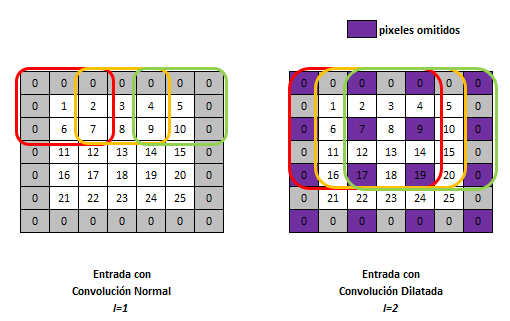
\includegraphics[scale=0.6]{Figs/Convolucion_dilatada.png}
	\caption{Ejemplo Convolución Dilatada \\Fuente: Elaboración Propia}
	\label{fig:cd}
\end{figure}

\section{Overfitting}

Un problema al momento de entrenar redes neuronales, es el \textit{overfitting}, el cual se da cuando la red neuronal en un momento específico del ciclo de entrenamiento no muestra un progreso en la capacidad de resolver problemas. Si no que solamente aprende una regularidad aleatoria dentro del conjunto de patrones de entrenamiento, esto quiere decir que la red está sufriendo un exceso de flexibilidad a la hora de agrupar los datos \cite{jabbar2015methods}.

\section{Underfitting}

Es lo contrario al \textit{overfitting}, siendo este cuando el modelo creado es incapaz de percibir variabilidad alguna en los datos. Dando como resultado que el clasificador resultante no tenga la capacidad de realizar una predicción aceptable \cite{jabbar2015methods}.

\section{Data Augmentation}
El Data augmentation consiste en la transformación de los datos existentes, para crear un \textit{dataset} con mayor cantidad de datos diferentes. El objetivo de esta herramienta es generar nuevos datos que puedan ser añadidos al conjunto ya existente, y así contar con más muestras para un mejor desempeño del algoritmo. Además de esto, también es implementado para reducir el \textit{overfitting}, ya que al añadir más información al conjunto de entrenamiento se evita que el modelo se sobre ajuste, normalmente esta técnica es implementada en problemas de clasificación donde el Dataset base del algoritmo no cuenta con una cantidad significativa de muestras para el entrenamiento de la red neuronal \cite{data}. \\



\section{Dropout}

El Dropout es una técnica de regularización implementada en el entrenamiento de redes neuronales, el fin de esta técnica es evitar que las neuronas que se encuentran en la red memoricen parte de la entrada, ya que si la red memoriza la entrada, se presentará un sobre ajuste en la red. El \textit{dropout} cumple su objetivo desactivando de manera aleatoria un porcentaje de las neuronas ubicadas en cada capa oculta \cite{drop}.

\section{Filtro de mediana}

Es una tecnología que procesa señales no lineales. El valor del ruido que proviene de la imagen digital o la secuencia es sustituida por el valor mediano de la vecindad (máscara).\\
Los pixeles de la máscara se clasifican en el orden de sus niveles de gris, el valor mediano del grupo es almacenado para sustituir el valor del ruido \cite{zhu2012improved}.

\section{Imagen Binaria} Una imagen binaria puede ser definida como una función de dos variables discretas [m, n], las cuales pueden tomar dos valores, \textit{0} o \textit{1}, de ahí su nombre de imagen binaria, estos valores pueden ser asignados dependiendo el nivel de gris que contenga la imagen (las imágenes binarias poseen dos niveles: blanco y negro). Las imágenes binarias son implementadas en visión artificial para realizar tareas de preprocesamiento de imágenes, el cual consiste en la eliminación del ruido y la simplificación del objeto que se encuentra en la imagen, además de esto, también se implementa para la descripción cualitativa de los objetos esto quiere decir que una imagen binaria facilita el cálculo de áreas, perímetros, diámetros, etc.\cite{ref_12}.

\section{Max pooling}

El pooling es conocido como una operación la cual permite analizar imágenes por regiones, el objetivo de esta operación es obtener la información más importante que se encuentra en las imágenes, esto se logra reduciendo la cantidad de datos que están presentes entre una capa y otra, una ventaja de implementar el \textit{max pooling} en las redes neuronales es que permite facilitar el procesamiento de las imágenes y el entrenamiento de la red sin perder información en el proceso.\\

Un operador \textit{max pooling}, se puede usar para la reducción del muestreo sobre las bandas de salida convolucionales, haciendo una reducción de la variabilidad. Esto lo realiza a través de un valor máximo de un grupo de \textit{R} activaciones.La \textit{m}-ésima banda de agrupación máxima está comprendido de \textit{J} filtros vinculados, como se muestra en la Ecuación ~\ref{eq:maxp}, dentro de un grupo de activaciones A. La banda máxima agrupada m está compuesta por f filtros relacionados $p_{m}=[p_{1m},...,p_{fm}] \in R^f$.

\begin{equation}
	\label{eq:maxp}
	p_{f,m}=max(h_{f,(m-1)N+r})
\end{equation}

Donde $N \in (1,...,R) $ representado como un desplazamiento de agrupación cuando $N < R$. La capa de agrupación disminuye la dimensionalidad de salida de K bandas convolucionales a $M=(K-R)/N+1$ bandas, que han sido agrupadas teniendo como resultante $p=[p1,...,pM] \in R^{M.J}$ \cite{gholamalinezhad2020pooling}, un ejemplo de max-pooling se puede observar en la Figura \ref{mp}.

\begin{figure}[ht]
	\centering
	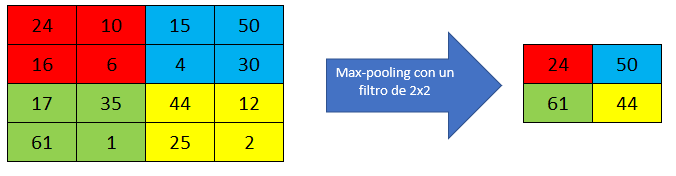
\includegraphics[scale=0.6]{Figs/mp.png}
	\caption{Ejemplo Max-Pooling\\Fuente: Elaboración Propia}
	\label{mp}
\end{figure}



\section{Padding}

El padding es un método utilizado con el fin de añadir píxeles de valor cero a los bordes de la imagen original, esto con el objetivo de que la imagen resultante al realizar la convolución sea del mismo tamaño que la original. Se debe tener en cuenta que si el padding no es implementado y se realiza la convolución, la imagen resultante será de un tamaño menor a la original, además este método permite la creación de redes más profundas y la extracción de características más especificas durante el entrenamiento.\\

El más usado es el \textit{zero padding}, debido a que mantiene la misma dimensionalidad al aplicar convoluciones. Por otro lado, permite a las redes neuronales convolucionadas codificar información de posición absoluta, a pesar de capas de agrupamiento en su arquitectura \cite{islam2021position}, un ejemplo de padding se puede observar en la Figura \ref{padding}.

\begin{figure}[ht]
	\centering
	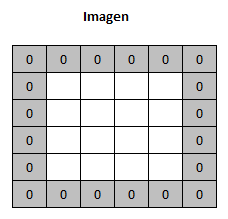
\includegraphics[scale=0.65]{Figs/padding.png}
	\caption{Ejemplo Zero Padding \\Fuente: Elaboración Propia}
	\label{padding}
\end{figure}

\section{Procesamiento de imágenes} El procesamiento de imágenes, se puede definir como la implementación de prácticas (disminuir el ruido, mejorar el contraste, ajustar el brillo, suavizar bordes, etc.), que buscan modificar ciertas características de la imagen con el fin de tener una mejor visualización de la misma, para realizar su posterior análisis de una manera más eficiente \cite{ref_13}.\\

El procesamiento de imágenes no tiene como objetivo incrementar la información que se puede obtener de las imágenes, pues el enfoque de esta técnica es resaltar las características más significativas que se encuentren en la imagen para que esta puede ser procesada de la mejor manera \cite{ref_13}.


\section{Stride}

Es un parámetro que especifica cuántos píxeles se traslada horizontalmente y verticalmente, mientras es convolucionada la imagen. En algunas arquitecturas el \textit{stride} se utiliza en vez de \textit{max pooling} para reducir el tamaño de la capa \cite{murphy2016overview}, un ejemplo de stride se puede observar en la Figura \ref{stride}.

\begin{figure}[ht]
	\centering
	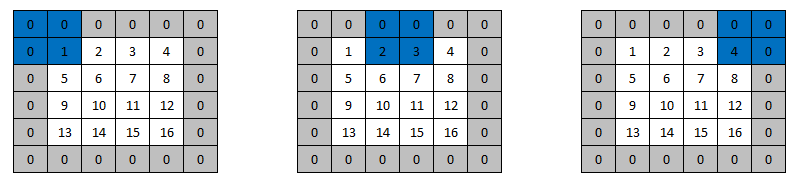
\includegraphics[scale=0.5]{Figs/stride.png}
	\caption{Convolución con Zero Padding y Stride $> 1$\\Fuente: Elaboración Propia}
	\label{stride}
\end{figure}

\section{Aprendizaje por transferencia}
El aprendizaje por transferencia, es definido por \textit{Lisa Torrey (2010)} como "\textit{la mejora del aprendizaje en una nueva tarea, a través de la transferencia de conocimientos de una tarea relacionada que ya se ha aprendido}". El objetivo del aprendizaje por transferencia es mejorar a un alumno con la transferencia de información de otro dominio relacionado. La mayor parte de algoritmos de aprendizaje automático fueron creados para ser empleados en tareas individuales \cite{ref_14}.

\section{Umbralización De una Imagen Digital}


Es un método que divide una imagen en grupos parecidos según un conjunto de criterios ya definidos. Podemos encontrar varias técnicas de \textit{umbralización} teniendo un enfoque primordial de la segmentación, especialmente en aplicaciones en las que la velocidad es fundamental en el proceso. \textit{umbralización} puede ser adaptativo al utilizarse diferentes umbrales para distintas regiones de la imagen \cite{kulkarni2012color}.

\section{Matriz De Confusión}

Una matriz de confusión en el ámbito del aprendizaje automático, se considera una herramienta utilizada para la visibilidad la eficacia de un algoritmo de aprendizaje supervisado. Toda columna de la matriz de confusión describe el número de predicciones de cada rango, por otra parte, las filas describen los casos de la categoría actual, en otras palabras, en la práctica nos concede observar cómo funciona el modelo de clasificación, junto con los errores y aciertos encuentra el modelo.\\

La matriz como se muestra en la Tabla \ref{table:Matriz}, se compone de términos de corrección de medidas estadísticas, llamados verdaderos positivos (VP), verdaderos negativos (VN), falsos positivos (FP) y falsos negativos (FN) \cite{maria2016performance}. 

\begin{table}[ht]
	\centering
	\begin{tabular}{|l|l|l|l}
		\cline{1-3}
		& \begin{tabular}[c]{@{}l@{}}Predicción\\ No\end{tabular}                                                & \begin{tabular}[c]{@{}l@{}}Predicción\\ Si\end{tabular}                                            &  \\ \cline{1-3}
		\begin{tabular}[c]{@{}l@{}}Real \\ No\end{tabular} & \begin{tabular}[c]{@{}l@{}}VN:\\ Predicción es negativo y \\ resultado real son positivos.\end{tabular} & \begin{tabular}[c]{@{}l@{}}FP:\\ Predicción es afirmativa\\ y la realidad es negativa.\end{tabular} &  \\ \cline{1-3}
		\begin{tabular}[c]{@{}l@{}}Real\\ Si\end{tabular}  & \begin{tabular}[c]{@{}l@{}}FN:\\ Predicción es negativa\\ y la realidad es negativa.\end{tabular}       & \begin{tabular}[c]{@{}l@{}}VP:\\ Predicción y resultado real\\ son positivos.\end{tabular}          &  \\ \cline{1-3}
	\end{tabular}
	\caption{Matriz de confusión}
	\label{table:Matriz}
\end{table}

La precisión alude a la cercanía entre la eficacia de una medición y el valor real. La forma de calcularse se muestra en la Ecuación \ref{eq:Exactitud}.

\begin{equation}
	Accuracy=\frac{VP+VN}{VP+VN+FP+FN}
	\label{eq:Exactitud}
\end{equation}

\chapter{Estado del arte}

\section{Selección Y Comercialización De Los Tubérculos Papa En Colombia}

La papa es un tubérculo conocido mundialmente, con una enorme producción y valores nutritivos, contiene muchos micro nutrientes primarios y cruciales como vitamina, vitamina B6, niacina, ácido fólico, potasio, hierro y magnesio, que es una fuente importante de carbohidratos, vitaminas y minerales para el ser humano. Según el plan de ordenamiento de la producción de papa en el país, presentado por el Ministerio de Agricultura y Desarrollo Rural en $2019$ \cite{informepapa2019}, en Colombia se siembran  $130 \ mil$ hectáreas y se producen cerca de  $2.8 \ millones$  de  toneladas  de  papa  al año. Los departamentos de Boyacá y Nariño constituyeron al año $2018$ un total de $24\%$ y $21\%$ de participación en la producción. En Boyacá el $95\%$ de la producción se destina al consumo fresco y el $5\%$ al procesamiento industrial. En Nariño los porcentajes son de $90\%$ para el consumo fresco y $10\%$ para el procesamiento industrial.\\

El procesamiento industrial de la producción de papa genera un valor agregado en comparación a la papa que se destina al mercado en fresco. El valor agregado depende del nivel en términos de lavado del producto, selección, clasificación y empaque. El plan de ordenamiento de la producción de papa en el país indica que un $25\%$ de la papa que se comercializa en fresco se comercializa con un valor agregado. El informe agrega también que "\textit{anualmente se  destina  aproximadamente  el  $6\%$  de  la  producción  nacional  al procesamiento industrial.  Existen en el país cerca de $50$ industrias dedicadas a la actividad de procesamiento de la papa, con diferente capacidad, diferentes niveles de desarrollo tecnológico y variada presencia en el mercado}".\\

El control de calidad actualmente se realiza de forma manual, realizado por personas, clasificando según su defecto y tamaño, esta acción tiene algunas desventajas: es subjetiva, laboriosa y lleva bastante tiempo, llevando a que la clasificación decaiga con el tiempo. En el trabajo publicado por \textit{Jender Mauricio Buitrago} en $2017$ \cite{recoleccionpapa}, se presenta un estudio de las prácticas agrícolas en el cultivo y comercialización de papa en la vereda Rechíniga en el departamento de Boyacá. Uno de los métodos utilizados, una vez se hace la recolecta del cultivo, es descrito como el método de bloque, que consiste en amontonar toda la papa producida en surcos y después los obreros se dividen el trabajo para clasificar el cultivo por tamaño, uno de los obreros se encarga de seleccionar la papa gruesa y otro la pareja para finalmente, empacarla en costales.\\

El estudio también menciona, que los campesinos de la vereda de Rechíniga, tienen en cuenta  el estado de la papa, el autor menciona que "\textit{en el proceso de extracción hay algunas que son tajadas por la herramienta utilizada para dicho proceso y se deben escoger y apartar para que no dañen las demás papas debido a que están más propensas a descomponerse fácil y rápidamente}".\\

Según el plan de ordenamiento de la producción de papa en el país, "\textit{la  papa  se  comercializa  en  Colombia  a  través  de  un  sistema  considerado  como altamente ineficiente tanto por el elevado número de niveles de intermediación como por la escasa o nula agregación de valor}", esto genera altos costos en los procesos de producción de materia prima en el procesamiento industrial de la papa. Debido a esto, desde el Ministerio de Agricultura y Desarrollo Rural se han presentado informes y estrategias para incluir la tecnología en los procesos de producción del sector papicultor del país.  

\section{MatLab}

Dentro de las técnicas de visión artificial para clasificar imágenes, se pueden usar diferentes ambientes de desarrollo como el ofrecido por MATLAB\textsuperscript{\textregistered}. Se tiene el trabajo de \textit{J. porras} \cite{article3}, en donde se menciona que la implementación de MATLAB\textsuperscript{\textregistered} como una herramienta de procesamiento de imágenes, radica en su facilidad para realizar cambios a las imágenes, es por esto que diseñó un sistema para la clasificación de objetos con base en su forma y color, usando métodos de visión artificial en MATLAB\textsuperscript{\textregistered}, con el uso de la librería \textit{ufm.dll}, para capturar y procesar imágenes. Se pudo evidenciar en los resultados del proyecto que \textit{J. porras} implementó, que utilizando técnicas de visión artificial se puede automatizar un proceso de producción con el fin de reducir tiempos y costos de operación en una planta de producción industrial. El artículo de \textit{C. Nandi} \cite{inproceedings} presenta una investigación, en donde, se consiguió calcular el tamaño de diferentes mangos, estimando el área cubierta en una imagen binaria, (imagen digital que tiene únicamente dos valores posibles para cada píxel), con base en el número de píxeles, luego de ser procesadas las imágenes, se clasificaron implementando un algoritmo basado en \textit{fuzzy logic}, teniendo en cuenta 5 variedades diferentes de mangos y como referencias el color de la cascara, tamaño, defectos superficiales, forma, firmeza, peso y olor.\\

\section{Redes Neuronales Artificiales}

Para la clasificación de imágenes usando técnicas de visión artificial, se tiene en primer lugar la literatura  acerca de las \textit{RNA} (\textit{Redes Neuronales Artificiales}). Las \textit{RNA} abarcan la temática del \textit{Deep Learning} \cite{lecun2015deep}, definido por \textit{LeCun (2015)}, como "\textit{el aprendizaje profundo permite que modelos computacionales compuestos por múltiples capas de procesamiento aprendan representaciones de datos con múltiples niveles de abstracción}". Estos métodos permiten la implementación de aplicaciones que permiten el reconocimiento visual y detección de objetos así como la predicción de datos estadísticos.\\ 

El trabajo de \textit{L. Pencue-Fierro y J. León Téllez} \cite{article2}, aborda una investigación hecha en Perú, en donde se aplicó visión artificial usando \textit{RNA} como método de clasificación de las principales características extraídas de las frutas, que son derivadas del análisis de las superficies, tanto en su contenido cromático como en la cantidad y distribución de defectos externos. La revista \textit{Multimedia Tools and Applications} \cite{Shrivastava2017} presentó una investigación, donde desarrollaron un sistema de visión artificial que usa un enfoque de categorización simplificado con un elevado índice de exactitud. El propósito del sistema es clasificar los granos de trigo de las especies \textit{triticum aestivum} y \textit{triticum durum} según sus propiedades visuales, usando una \textit{RNA} del tipo \textit{MLP}, (\textit{Multilayer Perceptron}); las imágenes se obtienen por medio de una cámara que captura las propiedades de tamaño, color y textura de cada grano con el objeto de que sirvan de acceso al procedimiento de categorización. El trabajo publicado por \textit{Ksh. Robert Singh y Saurabh Chaudhury} \cite{Singh2016}, en donde se propone el uso de redes neuronales \textit{BPNN}, (\textit{Back Propagation Artificial Neural Networks}), como método de clasificación y la descomposición mediante ondículas, (Tipo especial de transformada matemática que representa una señal en términos de versiones trasladadas y dilatadas de una onda finita), para clasificar los granos de arroz. El modelo de clasificación implemento una red neuronal \textit{BPNN} de cuatro capas la cual presento mejores resultados en comparación con otros métodos.\\

Usando el método de clasificación por \textit{RNA}, también se tiene el trabajo hecho por \textit{Krzysztof Koszela} \cite{Przybyl2019}, donde se presenta una forma para garantizar la correcta clasificación de los productos y reducir las pérdidas durante su almacenamiento. La investigación abarca esfuerzos centrados en la evaluación sensorial de patatas, con el análisis de imágenes por ordenador y la modelización neuronal \textit{RNA}. El objetivo de este estudio fue desarrollar un método para asistir a la identificación de cualquiera de las variedades y la turgencia de los tubérculos de patata, (Fenómeno que ocurre cuando una célula se dilata debido a la presión ejercida por los fluidos y por el contenido celular sobre las paredes de la célula), llevado a cabo sobre la base de los datos gráficos codificados en forma de imágenes digitales, obtenidos mediante algoritmos que interpretan los descriptores de imagen.\\

\section{Super Vector Machine}

El método de clasificación \textit{SVM} (\textit{Super Vector Machine}) revisado en la literatura, como el trabajo de \textit{Tao Liu} \cite{LIU201679}, en donde realizaron un proceso para analizar granos de arroz. El procedimiento usa $4$ fuentes de luz para crear la sombra del grano en $4$ direcciones; la diferencia en medio de las siluetas de los granos llenos y no llenos, se evalúa por medio del estudio de imágenes y un clasificador \textit{SVM}. El análisis se hace mediante el uso de imágenes \textit{RGB} (Red-Green-Blue), de los granos con las siluetas, luego se segmentan desde la imagen binaria, para sustraer información como el sector del grano y de la sombra. En el documento publicado por \textit{Chia-Lin} \cite{CHUNG2016404}, se menciona un método para clasificar plántulas (Embrión ya desarrollado como consecuencia de la germinación de una semilla), sanas e infectadas. Consiste en el análisis de imágenes mediante un escáner y el proceso de clasificación utilizando \textit{SVM}, en donde se hace uso de dos clasificadores, el primero distingue entre las plantas sanas y contaminadas, por otra parte, el segundo mide los niveles de contaminación. En el trabajo de \textit{Rillian Diello y Lucas Pires} \cite{PIRES201648}, se propuso un método de detección automática de enfermedad en cultivos de soja, el cual se basa en descripciones locales, conocido como el método \textit{BOV} (Bag of Values), luego de escanear la hoja. Se obtuvo a través de los vectores de entrada una clasificación en dos categorías, enfermo y sano, a partir de un clasificador \textit{SVM}. El trabajo de \textit{Chengming Sun y Tao Liu} \cite{SUN2014426}, propone un sistema para analizar el porcentaje de granos en el arroz que se encuentran en condiciones para ser distribuidos. El algoritmo se encarga de la división de los granos de manera automática. Tras la segmentación, es viable obtener el número de granos presentes en la imagen y la información específica, la exactitud del procedimiento puede verse afectada si el germen no se extrae del todo, por esa razón, el sistema detecta la viable región de germen y estima esta información usando \textit{SVM}.\\

\section{Otros métodos}

El trabajo hecho por \textit{Tao Liu y Wen Chen} \cite{LIU201682}, puso en práctica un método para controlar la población de pulgones, (Familia de insectos hemípteros), en el trigo, usando los métodos \textit{SVM}, el algoritmo \textit{MSER} (\textit{Maximally Stable Extremal Regions}), y el \textit{HOG} (\textit{Histogram of Gradients}). El uso de estos 3 métodos se conoce como \textit{SMH} (Unión entre \textit{SVM}, \textit{MSER} y \textit{HOG}), se basa en el análisis de imágenes tratadas a partir de unos parámetros, con la finalidad de detectar la presencia y/o ausencia de pulgones, se hizo uso de este método a partir del color y la densidad de población. Al comparar este método con otros cinco comúnmente utilizados, los resultados presentaron un rendimiento superior en la identificación de pulgones. \\

El trabajo publicado por \textit{Rodica Sobolu} \cite{sobolu2020automatic}, propone un algoritmo de clasificación automática de patatas. Se realizaron dos tipos de clasificación: una en función del tamaño de las patatas y otra en función de su calidad. La segmentación de las zonas defectuosas se hizo mediante métodos como \textit{global thresholding}, para extraer características morfológicas y estadísticas de las zonas segmentadas. Estas características se eligieron como entradas para los algoritmos de clasificación usando métodos como \textit{SVM}, \textit{Decision  Tree} y \textit{LDA} (\textit{Linear Discriminant Analysis}), implementados en MATLAB\textsuperscript{\textregistered} \textit{Classification Toolbox}. Se llegó a la conclusión de que el método de \textit{SVM} ha clasificado las patatas según su tamaño con una mayor tasa de éxito y en la clasificación por calidad, el método \textit{LDA}.\\

Se encuentran unos métodos poco comunes en la literatura, como por ejemplo los presentados en el artículo de \textit{Alberto Martines Rodriguez} \cite{article5}, donde se identificaron objetos en movimiento mediante la ayuda de la visión artificial y la transmisión de datos a un brazo robótico implementando \textit{C++} y \textit{Open CV}, usando el código de cadena, (Actualmente el grupo de reconocimiento de patrones e inteligencia artificial aplicada), para calcular las características de los objetos por color y forma. También, el artículo hecho por \textit{L. Han y M. S. Haleem} \cite{7237209}, propone un algoritmo de detección automática de enfermedades en los cultivos, utilizando para este proceso el algoritmo \textit{MCW} (\textit{Marker-Controlled Watershed}) para separar el fondo de la imágene, de la hoja del cultivo. \textit{El SLIC} (\textit{Simple Linear Iterative Clustering}), se utilizó para obtener las características presentadas por la enfermedad sobre la planta y por ultimo, la clasificación y textura se obtienen a través de \textit{GLCM} (\textit{Gray Level Co-occurrence Matrix}), el modelo de clasificación fue el \textit{SVM}, este método propuesto presento un mayor rendimiento.\\

El trabajo presentado por \textit{Michael Barnes y Tom Duckett} \cite{Barnes2010}, cuyo objetivo de  investigación es introducir un método automático de detección de manchas en imágenes digitales de patatas. El sistema desarrollado es entrenable, de modo que pueda trabajar con diferentes variedades de patatas y variaciones en las estaciones, condiciones de iluminación, etc. Otro objetivo, pensando en su posible implantación en entornos industriales, es permitir el procesamiento de imágenes en tiempo real, posiblemente mediante la construcción de \textit{Minimalist Boosted Classifier}, que extraigan un subconjunto mínimo de todas las características que optimicen el rendimiento de la detección con el menor coste computacional posible.


\section{Clasificación De Papa Con Técnicas De Aprendizaje Profundo}

\textit{Elsharif, Abeer} presenta el desarrollo de una red neuronal convolucional  para la clasificación de $4$ variedades de tubérculos de papa en un \textit{dataset} de $2400$ imágenes \cite{elsharif2020potato}. Los resultados de la implementación de la red fueron de casi un $100\%$ para una única característica, es te caso, la variedad a la que pertenece el tubérculo. \textit{Noordam, J.} presenta un proyecto para la clasificación en alta velocidad de tubérculos de papa de acuerdo a una inspección de calidad a partir del color y el tamaño \cite{noordam2000high}. En este proyecto utilizaron algoritmos de clasificación basados en la segmentación por color de las papas, debido a esto únicamente utilizaron defectos que puedan ser evidenciados por el color. Usaron los algoritmos de \textit{Multi-layer feed-forward Neural Networks} (MLF-NN) y \textit{Linear Discriminant Analysis} (LDA) con los que obtienen resultados superiores al $95\%$ en las predicciones hechas.\\

\textit{Paul, H.} presenta su trabajo, donde desarrollan una estación de inspección automatizada para verificar la calidad de las papas \cite{heinemann1996automated}. La estación fue creada para el departamento de agricultura de Estados Unidos, consiste de una recámara para la toma de imágenes, banda transportadora, cámara, unidad de selección y análisis, un computador y equipo de control. La estación de inspección clasifica las papas de acuerdo a su forma y tamaño mediante el uso de an algoritmo conocido como \textit{algoritmo de rastreo de 8 vecinos} para encontrar los puntos principales que componen la forma del tubérculo analizado. Obtuvieron resultados de $88\%$ para imágenes en movimiento.









\chapter{Diseño Del Algoritmo de Clasificación}


Se diseñó un algoritmo de clasificación utilizando Redes Neuronales Convolucionales y técnicas de visión artificial con la librería \textit{OpenCV}, que es una biblioteca de software de código abierto para realizar visión por computador y aprendizaje automático, para clasificar las características de tipo, daño y tamaño en tubérculos de papa. El Procedimiento que se llevó acabo se presenta en la Figura \ref{fig:flujogeneral}. Las características de tipo y daño serán analizadas con la red neuronal artificial y, la característica de tamaño, será analizada con el uso de \textit{OpenCV}. De esta manera, ambos análisis dan como resultado la clasificación de la papa según las características de calidad definidas. \\

\begin{figure}[ht]
	\centering
	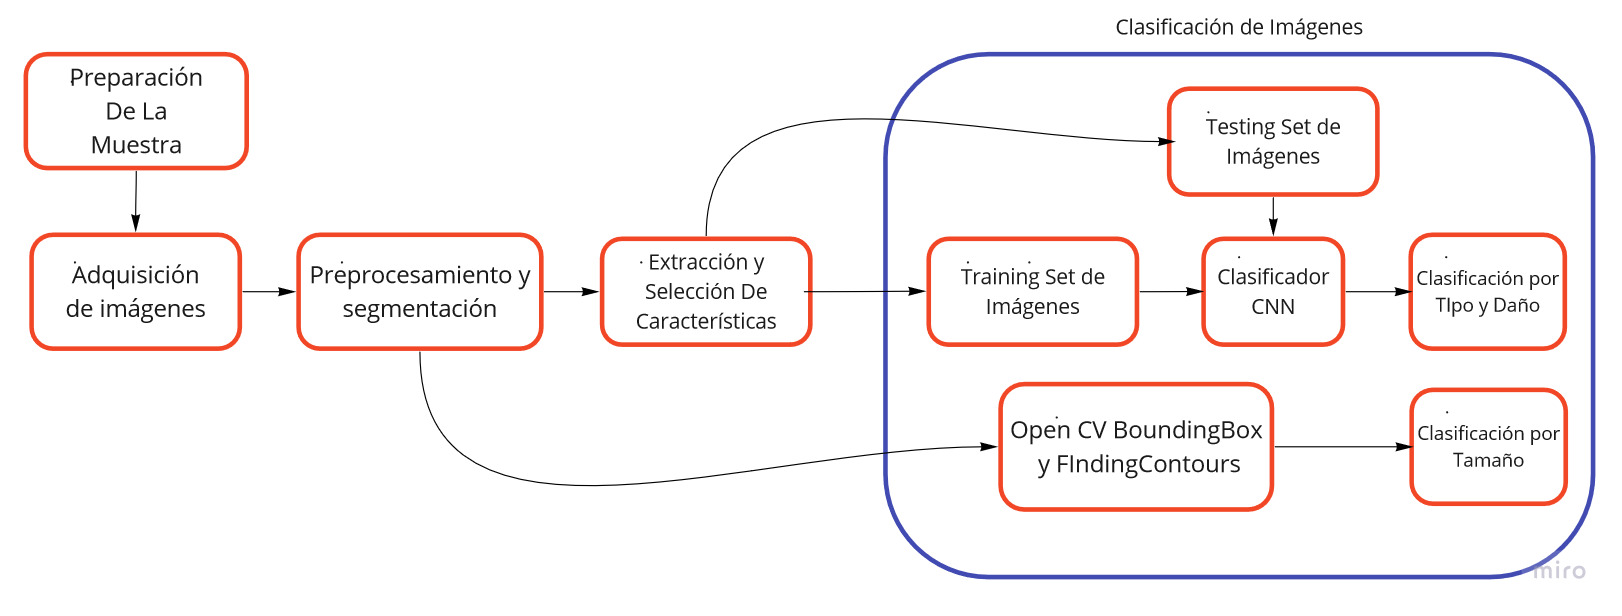
\includegraphics[scale=0.28]{Figs/FGGeneral.jpg}
	\caption{Arquitectura del Sistema de Clasificación \\ Fuente: Elaboración Propia}
	\label{fig:flujogeneral}
\end{figure}

La estrategia propuesta para realizar la clasificación de tubérculos de papa en este documento, consiste desde la adquisición de muestras y creación de un \textit{dataset} de tubérculos de papa, hasta el diseño de un algoritmo de clasificación con Redes Neuronales, utilizando la librería \textit{Pytorch}, que es una biblioteca de software para la aplicación de aprendizaje profundo, y la librería de\textit{OpenCV} en el lenguaje de programación de \textit{Python}. El algoritmo de clasificación será implementado en un prototipo de banda transportadora, que permita el movimiento del elemento por debajo de una cámara, para ser analizado y clasificado. Los sistemas de visión artificial utilizados en inspecciones visuales, permiten que la operación sea más eficiente si la producción requiere que el proceso aumente en velocidad, cantidad de producción y se encuentre en funcionamiento las 24 horas del día o la repetibilidad de las medidas \cite{artificial2012aplicacion}.\\

Según la norma $NTC \ 341-3$, se considera que el daño en una papa es "\textit{una lesión o alteración de magnitud variable que presentan los tubérculos}", se establecen $5$ tipos de daños, sin embargo, los tubérculos seleccionados para el proyecto pertenecen a los siguientes tipos de daño, definidos según la norma. Las papas fueron clasificadas por los desarrolladores del proyecto de acuerdo a los parámetros de la norma.

\begin{itemize}
	\item Daños Mecánicos: Lesiones causadas por agentes físicos, Figura \ref{fig:dano1}.
	
	\begin{figure}[ht]
		\centering
		\includegraphics[scale=0.04]{Figs/daño1.JPG}
		\caption{Muestra de Papa Clasificada en Daño Mecánico \\ Fuente: Elaboración Propia}
		\label{fig:dano1}
	\end{figure}
		
	\item Daños y Defectos Fisiológicos: Lesiones o defectos que provienen de alteraciones no patogénicas de origen interno o externo, Figura \ref{fig:dano2}.
	
	\begin{figure}[ht]
		\centering
		\includegraphics[scale=0.04]{Figs/daño2.JPG}
		\caption{Muestra de Papa Clasificada en Daño Fisiológico \\ Fuente: Elaboración Propia}
		\label{fig:dano2}
	\end{figure}

	\item Daños Causados Por Insectos: Se presentan en forma de túneles o galerías de diámetro y longitud variable causados por insectos y moluscos, Figura \ref{fig:dano3}.
	
	\begin{figure}[ht]
		\centering
		\includegraphics[scale=0.04]{Figs/daño3.JPG}
		\caption{Muestra de Papa Clasificada en Daño Causado Por Insecto \\ Fuente: Elaboración Propia}
		\label{fig:dano3}
	\end{figure}
\end{itemize}

Se considera un tubérculo en buen estado aquel, que de acuerdo a la norma, no presenta ninguno de las daños descritos anteriormente, como el tubérculo que se presenta en la Figura \ref{fig:good}.

\begin{figure}[ht]
	\centering
	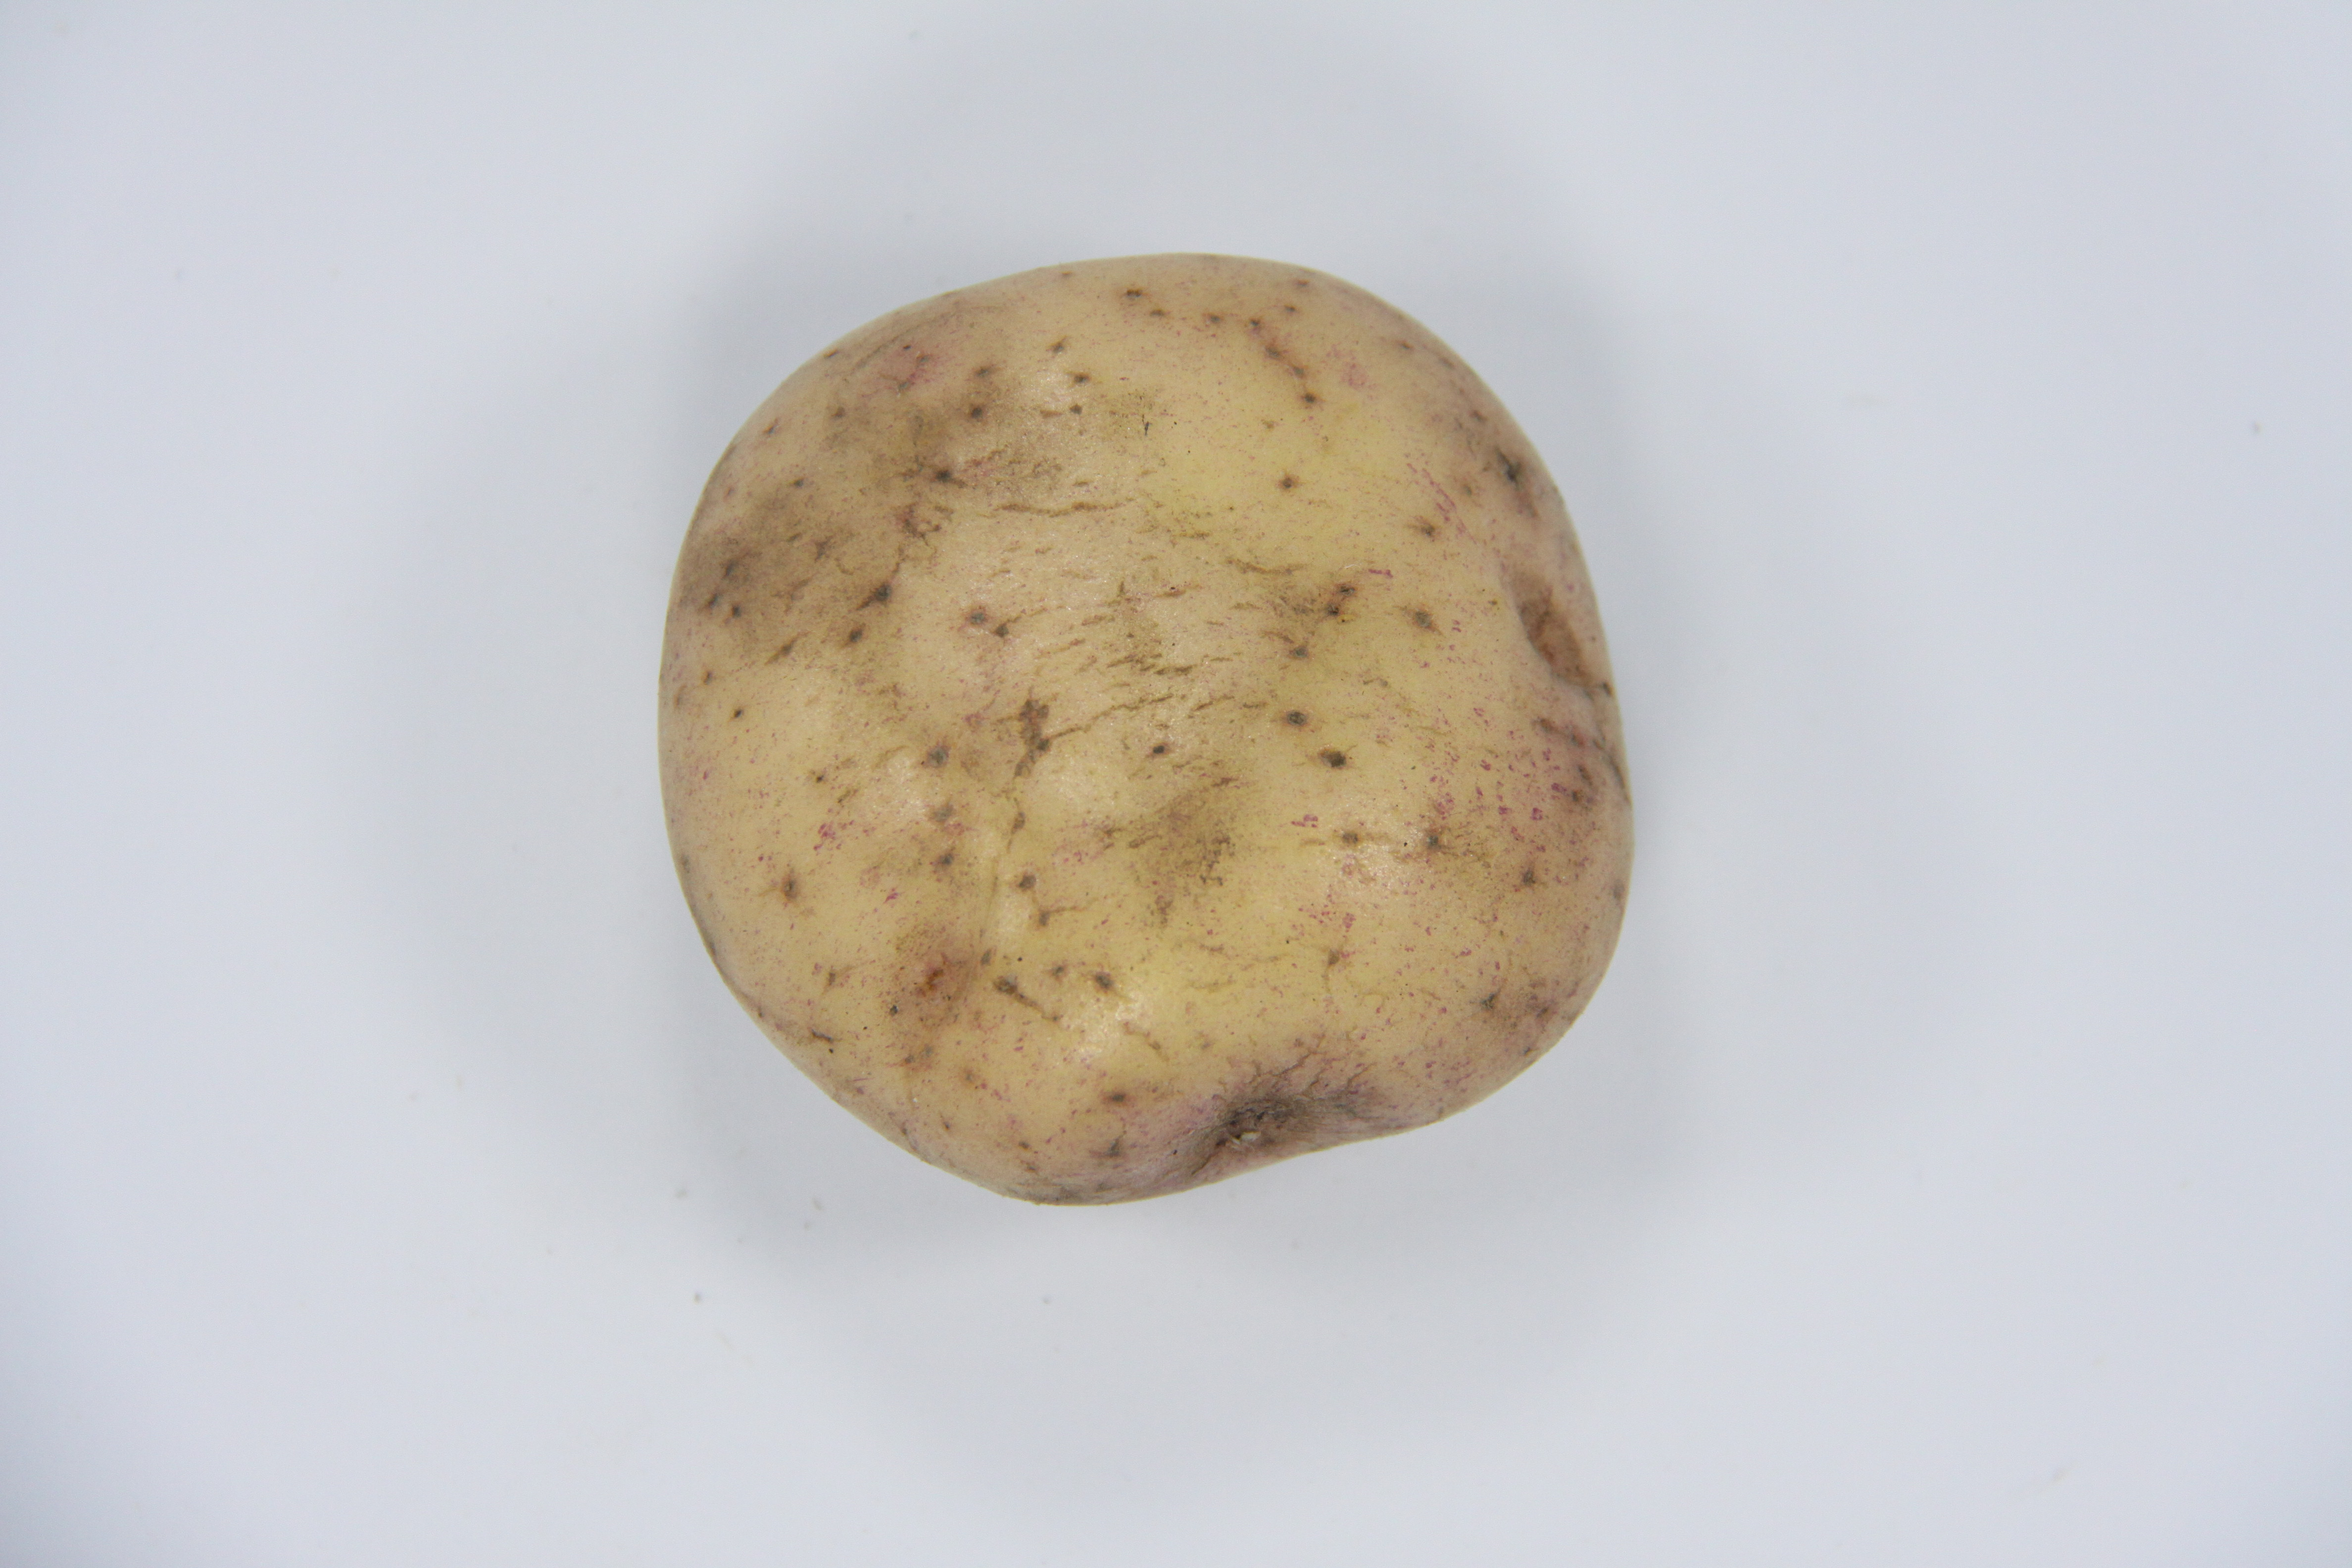
\includegraphics[scale=0.04]{Figs/good.JPG}
	\caption{Muestra de Papa Clasificada en Buen Estado \\ Fuente: Elaboración Propia}
	\label{fig:good}
\end{figure}

De igual forma, la norma define el diámetro como "\textit{la máxima distancia tomada en ángulos rectos sobre el eje más largo del tubérculo}", se establecen $4$ tamaños según el diámetro, sin embargo, los tubérculos seleccionados para el proyecto serán clasificados por los tamaños presentados en la Tabla \ref{tamano}, establecidos según la norma.\\

\newpage
\begin{table}[ht]
	\centering
	\begin{tabular}{|c|c|}
		\hline
		Denominación & Diámetro en mm \\ \hline
		Muy Grande   & Mayor a 90     \\ \hline
		Grande       & 65 - 90        \\ \hline
		Mediana      & 45 - 64        \\ \hline
	\end{tabular}	
	\caption{Clasificación Por Tamaño del Tubérculo}
	\label{tamano}
\end{table}

Los tubérculos que serán analizados en el prototipo deben estar limpios. La norma define una papa limpia como "\textit{los tubérculos libres de tierra u otras impurezas adheridas}". Debido a que una de las características que indica el tipo de tubérculo es el color, en este caso, se usarán los tubérculos de la variedad \textit{R12} y \textit{Pastusa}, es por esto que se deben tener los tubérculos limpios. 

\section{Preparación y Adquisición De Las Imágenes}

Se seleccionó un total de $592$ tubérculos de papa, que manualmente fueron clasificados en tres categorías definidas. Las etiquetas de cada imagen se encuentran dentro del nombre de cada archivo, que corresponde al \textit{metadata} de cada foto tomada. Definido de la siguiente manera:

\begin{itemize}
	\item \textit{Tipo:} Pastusa o R12 $[0,1]$
	\item \textit{Daño:} Buena y Defectuosa $[0,1]$
	\item \textit{Tamaño:} Muy grande, Grande y Mediana $[0,1,2]$
	\item \textit{Numero de la Imágen} Etiqueta asignada por la cámara.
\end{itemize}	

Las fotos tomadas para la creación del \textit{dataset}, poseen un tamaño de $(3168, 4752)$ pixeles. Fueron tomadas con una cámara profesional de referencia \textit{Canon EOS 50D}, que tiene 15.1 mega pixeles de resolución y se puede ajustar la sensibilidad \textit{ISO} desde $100$ hasta $3200$. La cámara fue configurada con \textit{ISO-800} que corresponde al parámetro de sensibilidad del sensor de ruido de la cámara, una velocidad de obturación de $\frac{1}{640}$ segundos, que corresponde al dispositivo que controla el tiempo en el que la luz incide sobre el sensor de la cámara, y finalmente una apertura de diafragma de $F-7.1$ que corresponde a la apertura del lente que deja pasar la luz \cite{Camara}, tener en cuenta que a mayor apertura de diafragma, menor luz se deja pasar. Se construyó una caja con iluminación fija la cual se muestra en la Figura \ref{fig:chamber} usando bombillos de luz blanca de $6500$ Kelvin de temperatura de color, para que la iluminación en todas las fotos tomadas fuera uniforme según la norma española \textit{UNE-EN 12464-1} \cite{normaespanola}.

\newpage
\begin{figure}[ht]
	\centering
	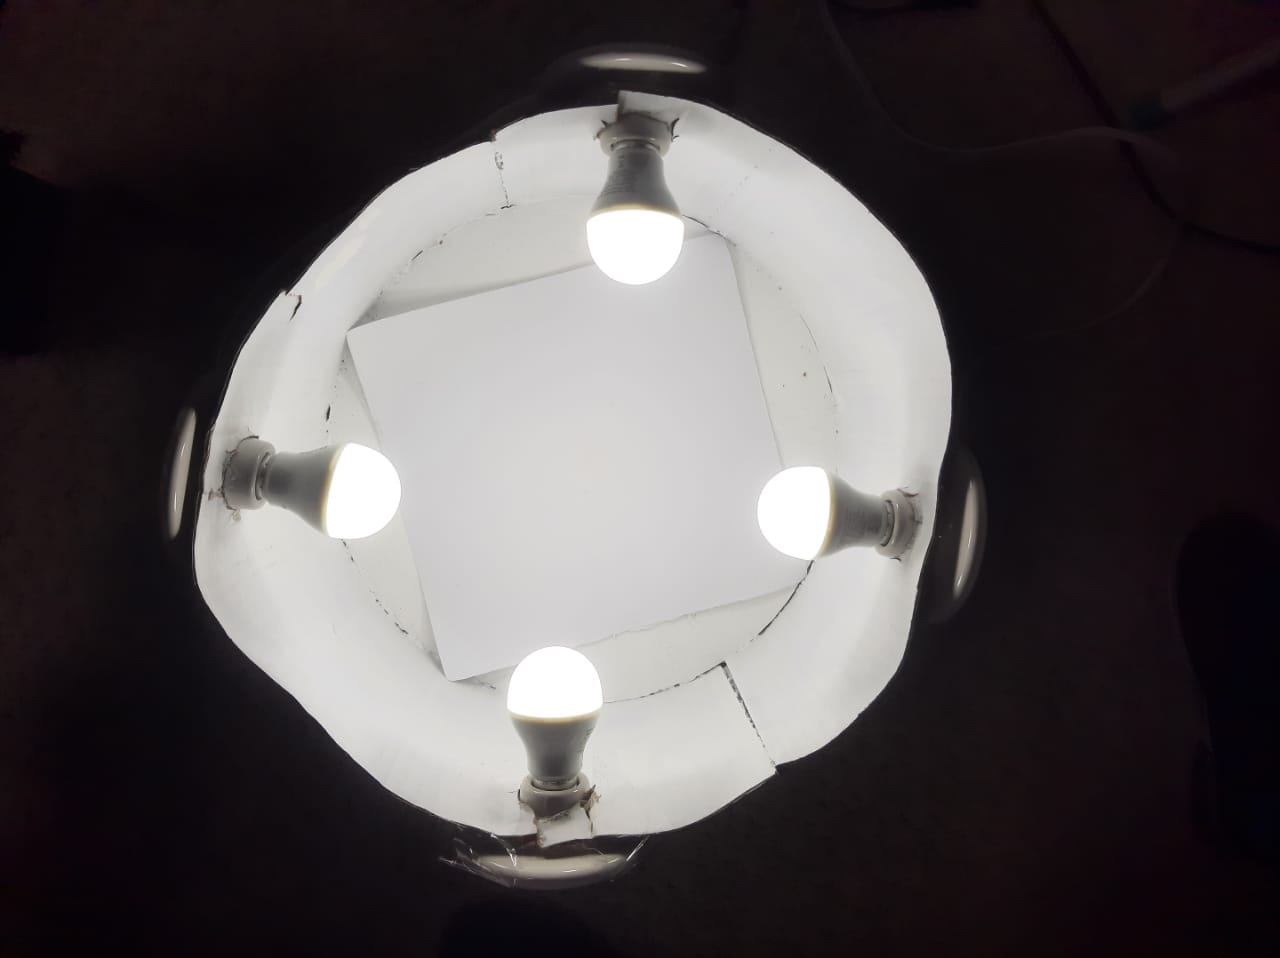
\includegraphics[scale=0.16]{Figs/Chamber.JPEG}
	\caption{Récamara Para la Toma de Fotos\\ Fuente: Elaboración Propia}
	\label{fig:chamber}
\end{figure}


La cámara para la toma de las fotos fue fijada a un trípode ubicado a $30 \ cm$ desde el lente hasta la parte superior de la muestra, ya que al tener tubérculos de diferentes tamaños, se puede garantizar que los píxeles que definen el perímetro de las muestras son uniformes sin importar el tamaño del tubérculo. Utilizando la librería \textit{Pandas} de \textit{Python}, se creó un \textit{Dataframe} que contiene el metadata de cada imagen. En la Tabla \ref{table:metadata} se puede apreciar la distribución del \textit{MetaData} de las imágenes almacenas en el \textit{Dataset}, donde se toman cinco imagenes al azar como muestra. A partir de esta tabla se crea un archivo \textit{.CSV} donde se encuentra la información de las 592 imágenes.\\

\begin{table}[ht]
	\centering
	\begin{tabular}{|c|c|c|c|}
		\hline
		Tipo & Daño & Tamaño & Filename \\
		\hline
		R12 & Defectuosa & Grande & 1\_1\_1\_075.JPG \\
		\hline
		PASTUSA & Buena & Grande & 0\_0\_1\_1973.JPG \\
		\hline
		R12 & Buena & Grande & 1\_0\_1\_2054.JPG \\
		\hline
		PASTUSA & Buena & Mediana & 0\_0\_2\_2042.JPG \\
		\hline
		PASTUSA & Buena & Grande & 0\_0\_1\_1955.JPG \\
		\hline
	\end{tabular}	
	\caption{MetaData de 5 Imágenes de Muestra}
	\label{table:metadata}
\end{table}


Una vez la información de cada imagen fue guardada en el archivo \textit{metadata.csv}, se agruparon las posibles combinaciones de las características de \textit{Tipo} y \textit{Daño}, para definir las \textit{clases} dentro de la red neuronal. Para realizar este proceso, se creó una condición dentro del \textit{Dataframe}, que contiene el \textit{metadata} para generar una columna adicional con la información de la Tabla \ref{table:Clases}. De esta forma se definieron las $4 \ clases$ que serán entrenadas en la red neuronal, para el posterior proceso de clasificación por visión artificial. \\	

\newpage
\begin{table}[ht]
	\centering
	\begin{tabular}{|c|c|c|c|c|c|}
		\hline
		PASTUSA & R12 & Buena & Defectuosa & Clase & Cantidad De Muestras\\
		\hline
		X &  & X &  & CLASE 1 & 140\\
		\hline
		X &  &  & X & CLASE 2 & 110\\
		\hline
		& X & X &  & CLASE 3 & 106\\
		\hline
		& X &  & X & CLASE 4 & 236\\
		\hline
	\end{tabular}	
	\caption{Clases Definidas}
	\label{table:Clases}
\end{table}	

\section{Distribución del Dataset}

La librería \textit{Plotly}, que permite realizar gráficas en \textit{Python}, presenta la distribución en porcentaje de las imágenes pertenecientes a cada característica definida en el \textit{dataset} como se muestra en la Figura \ref{fig:distribuciontipo}.\\


\begin{figure}[ht]
	\centering
	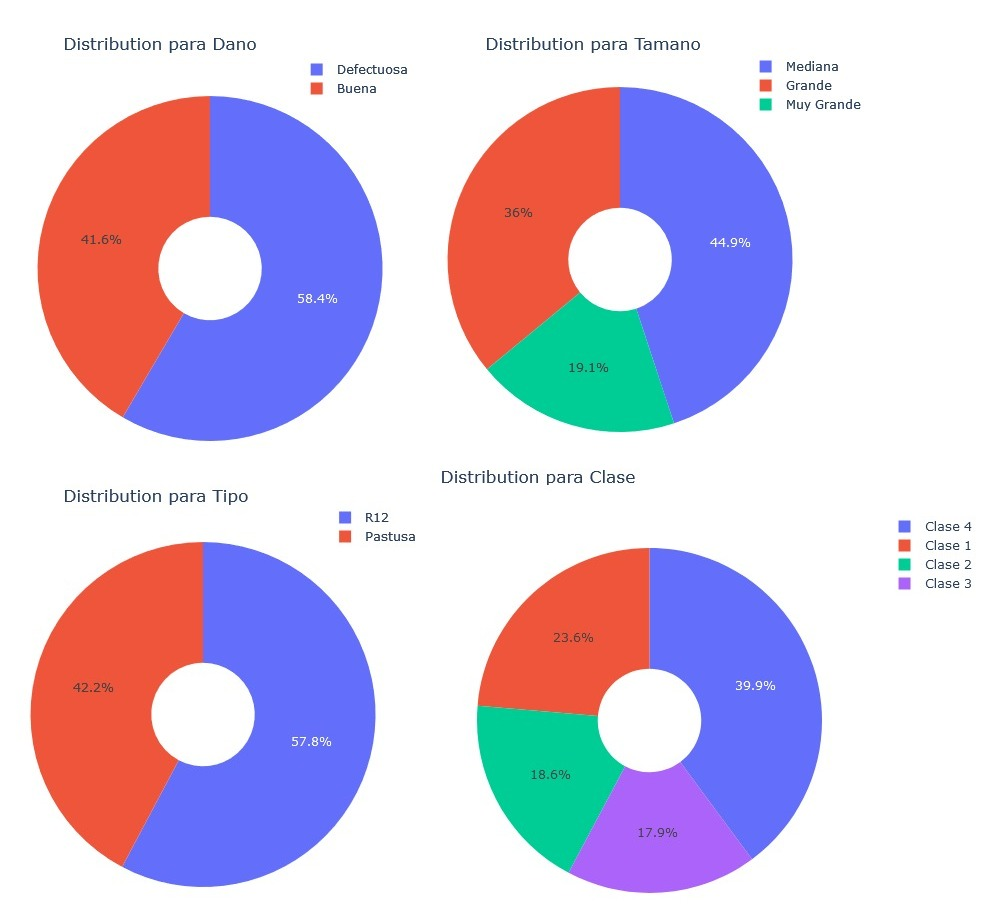
\includegraphics[scale=0.42]{Figs/Distribucion.jpg}
	\caption{Distribución del Dataset Según Sus Características Y Clases Definidas \\ Fuente: Elaboración Propia}
	\label{fig:distribuciontipo}
\end{figure}

\newpage
Se definieron los conjuntos de \textit{entrenamiento} y \textit{validación}, a partir del archivo \textit{metadata.csv} de la Tabla \ref{table:metadata}. Se utilizó $80\%$ para \textit{entrenamiento} y $20\%$ para \textit{validación}. Se crearon los archivos \textit{train.csv} y \textit{test.csv} que contienen el \textit{metadata} y la dirección de las imágenes separadas en el respectivo $80\%$ y $20\%$.\\

\section{Optimización Bayesiana}

La mayor parte de modelos implementados en \textit{machine learning} poseen una serie de parámetros que no pueden ser aprendidos de los datos, es por esto que deben ser establecidos antes del entrenamiento. Estos parámetros son conocidos como hiperparámetros. \\

Dos de las estrategias más empleadas para probar diferentes combinaciones de hiperparámetros y evaluarlas mediante métodos de validación, son \textit{grid search y random search} \cite{liashchynskyi2019grid}. En la estrategia de \textit{grid search}, los valores estudiados de cada hiperparámetro, son distribuidos uniformemente dentro de un rango delimitado por el analista. En la estrategia de \textit{random search}, los datos son aleatorios dentro de ese rango como se muestra en la Figura \ref{fig:Hiperparámetros grid search y random search}.

\begin{figure}[ht]
	\centering
	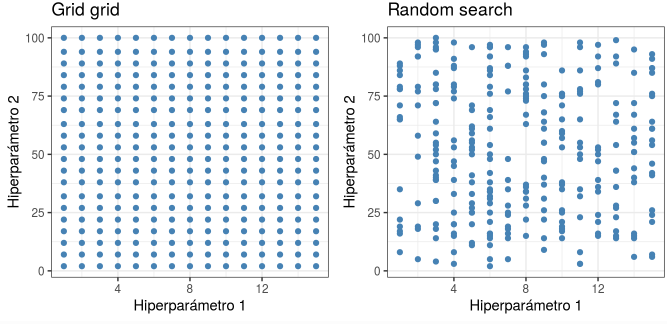
\includegraphics[scale=0.6]{Figs/121.png}
	\caption{Métodos de Optimización De Hiperparámetros \\Fuente: Amat, J. (2020)}
	\label{fig:Hiperparámetros grid search y random search}
\end{figure}

A pesar de que las dos estrategias son válidas y se obtienen buenos resultados, sobretodo cuando se tiene criterio para acotar el rango de búsqueda, poseen una carencia similar: ninguna de las dos tiene en cuenta los resultados obtenidos hasta el momento, lo cual impide que se focalicen en la búsqueda de las regiones de mayor interés y evitando las regiones innecesarias.\\

Otro método utilizado para la búsqueda de los hiperparámetros de un modelo es la optimización bayesiana, definido por \textit{Peter Frazier (2018)} \cite{frazier2018tutorial} como \textit{"crear un modelo probabilístico en el que el valor de la función objetivo es la métrica de validación del modelo, en este caso, la precisión}. Con este método, se logra que la búsqueda se vaya redirigiendo en cada iteración hacia las regiones de mayor interés. Esto con el fin de reducir el número de combinaciones de los hiperparámetros con los que el modelo es evaluado, seleccionando únicamente los mejores candidatos. Esto significa que, la ventaja frente a las estrategias descritas anteriormente, se maximiza cuando el espacio de búsqueda es muy amplio o la evaluación del modelo es muy lenta.\\

Para realizar la optimización bayesiana, se utilizó el módulo para \textit{Python} \textit{Botorch}  \cite{balandat2020botorch}. Es el motor de optimización de \textit{Ax-Services} compatible con \textit{Pytorch}, que admite algunas funciones de minimización y maximización, como la mejora esperada (\textit{EI}), la probabilidad de mejora y el límite superior de confianza. \textit{EI} es una función de adquisición que recompensa la evaluación del objetivo $f(x)$, basándose en la mejora esperada en relación con el mejor momento $f*$. La Ecuación \ref{EI}, define el comportamiento de la mejora esperada.

\begin{equation}
	{EI(x)=\in[max(f(x)-f*),0]}
	\label{EI}
\end{equation}

El resultado de la parametrización, se selecciona y se evalúa en el siguiente paso. Una vez que se ha explorado adecuadamente el espacio de los parámetros, la mejora esperada se estrecha naturalmente en las ubicaciones donde hay una alta probabilidad de un buen valor objetivo. Este proceso se realiza por $20$ etapas, en las que se varían los parámetros de acuerdo a lo descrito anteriormente. 


\chapter{Algoritmo de Clasificación}

\section{Red Neuronal Convolucional}

La arquitectura general de una red neuronal convolucional (\textit{RNC}) se muestra en la Figura \ref{fig:cnnarchitecture}, que consiste en varias capas de procesamiento de imágenes en donde se realizan convoluciones (operación matricial en la entrada de a red ue extrae características y disminuye la complejidad del modelo) \cite{o2015introduction}. Se realizaron pruebas con las arquitecturas de (\textit{RNC}) pre entrenadas \textit{Alexnet}, \textit{Resnet18}, \textit{VGG11} y \textit{VGG19} y se implementó la optimización bayesiana en ciertos hiperparámetros de las arquitecturas existentes, para mejorar los resultados.

\vspace{1cm}

\begin{figure}[ht]
	\centering
	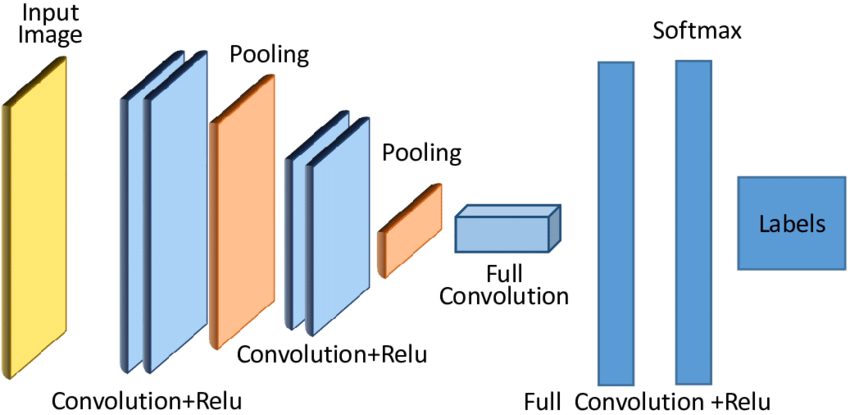
\includegraphics[scale=0.8]{Figs/A-generic-CNN-Architecture.png}	
	\caption{Arquitectura General De Una \textit{RNC} \\ Fuente: O'Shea, K. (2015)} 
	\label{fig:cnnarchitecture}
\end{figure}	

\vspace{0.5cm}

El procedimiento realizado para implementar la red neuronal convolucional se aprecia en la Figura \ref{fig:procedimiento}, donde se indican los pasos a seguir previo a utilizar alguna de las arquitecturas pre entrenadas. Cada ítem será descrito en las próximas secciones.  

\newpage
\begin{figure}[ht]
	\centering
	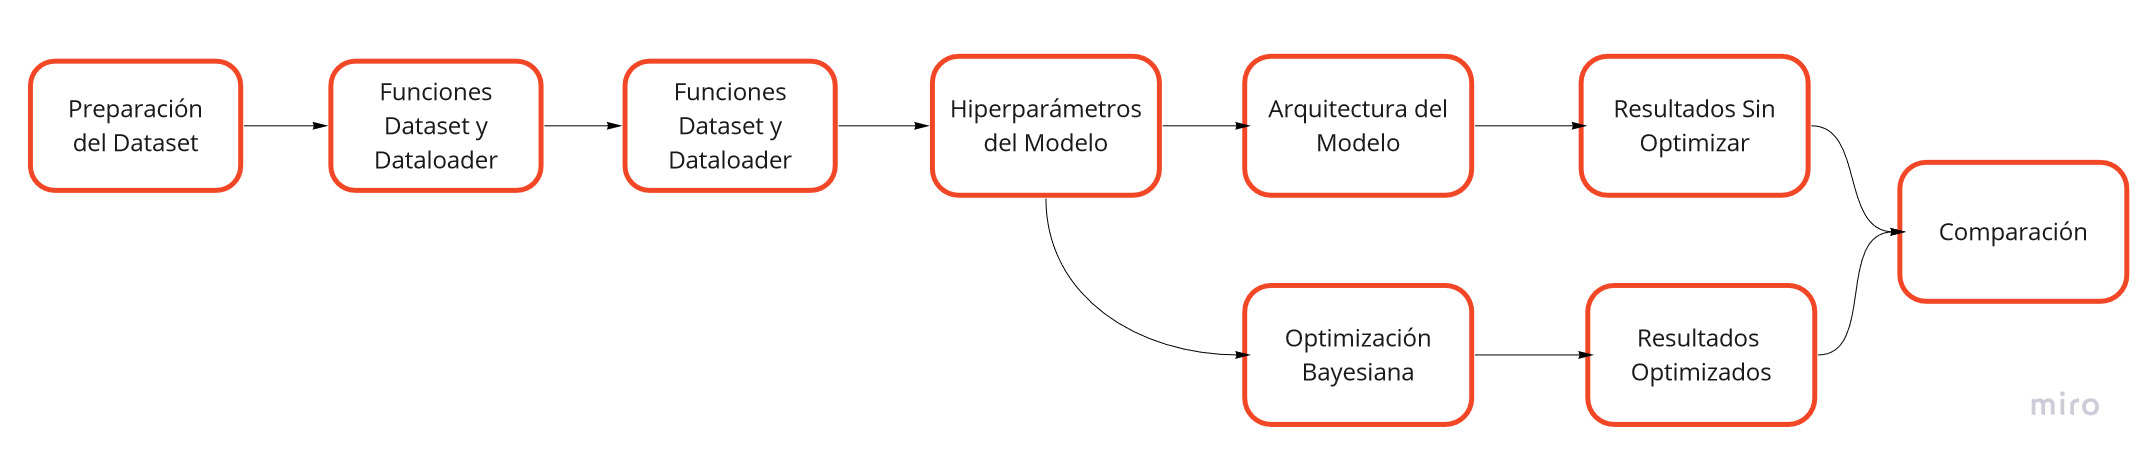
\includegraphics[scale=0.4]{Figs/procedimiento.jpg}
	\caption{Procedimiento Para Implementar La \textit{RNC} \\ Fuente: Elaboración Propia}
	\label{fig:procedimiento}
\end{figure}	

\subsection{Preparación Del \textit{Dataset}}

Para realizar un correcto entrenamiento del modelo de red neuronal convolucional es necesario aplicar un preprocesamiento a las imágenes, para que el modelo extraiga características pertinentes a las clases definidas. En este apartado se explica el procedimiento que se lleva a cabo para el preprocesamiento de imágenes y los diferentes filtros aplicados para realizar el \textit{Data Augmentation}.

\subsubsection{PREPROCESAMIENTO DE IMÁGENES}

Usando el módulo \textit{tranforms.compose()}, de la librería \textit{Pytorch}, se pueden encadenar unas determinadas funciones que aplican diferentes tipos de filtros y transformaciones al \textit{Dataset} \cite{Pytorch}. De esta forma, se crea la tarea de segmentación debido a que las transformaciones aumentan en consideración el tamaño original del \textit{Dataset}, facilitando así, la extracción de características.\\

En la Tabla \ref{table:Filters1} se observa una parte de las transformaciones de imágenes disponibles en el módulo \textit{torchvision.tranforms.compose} de la librería \textit{Pytorch}. En el caso del \textit{Dataset} de papas creado, se deben tener en cuenta únicamente las transformaciones cuyo resultado sea relevante para la extracción de características de la imágen, por ejemplo, como se explicó anteriormente, se va a clasificar el tubérculo de papá en tipo y daño, con la red neuronal, por este motivo, el color es una característica que define si la papa pertenece a la clase \textit{R12} o \textit{Pastusa} y, en algunos casos, si se encuentra con algún tipo de daño, por este motivo, los filtros que transforman la imágen en escala de grises no son relevantes y podrían afectar el rendimiento del algoritmo.

\newpage

\vspace{1cm}

\begin{table}[ht]
	\centering
	\begin{tabular}{|p{3cm}|p{4cm}|p{3.8cm}|p{4cm}|}
		\hline
		Image Transform       & \multicolumn{1}{c|}{Use}                                                               & Image Transform       & \multicolumn{1}{c|}{Use}                                                                        \\ \hline
		CenterCrop            & Recorta la imagen en el centro                                                         & RandomResizedCrop     & Recorta una porción aleatoria de la imágen y la redimensiona a un tamaño determinado            \\ \hline
		ColorJitter           & Cambia aleatoriamente el brillo, el contraste, la saturación y el tono de una imagen   & RandomRotation        & Rota la imagen a un ángulo determinado                                                          \\ \hline
		FiverCrop              & Recorta la imagen en cuatro esquinas y el recorte central                              & RandomVerticalFlip    & Voltea verticalmente la imagen al azar con una probabilidad dada                                \\ \hline
		Grayscale             & Convierte la imágen en escala de grises                                                & Resize                & Redimensiona la imagen al tamaño dado                                                           \\ \hline
		Pad                   & Rellena la imágen en todos sus lados con el valor de \textit{pad} dado                        & TenCrop               & Recorta la imagen dada en cuatro esquinas y el recorte central \\ \hline
		RandomAffine          & Transformación aleatoria de la imagen manteniendo el centro invariante            & GaussianBlur          & Desenfoca la imágen con un filtro gausseano                                                                                                                     \\ \hline
	\end{tabular}
	\caption{Funciones de transformación de imágenes del módulo de \textit{Pytorch}}
	\label{table:Filters1}
\end{table}

\vspace{0.5cm}

De igual forma, en la Tabla \ref{table:filters2} se observan algunos filtros como recortes en la imagen, rotaciones, cambios de perspectiva, cambios en la nitidez y contraste de la imagen. El uso de los filtros en la fase de preprocesamiento permite enriquecer el \textit{dataset} para garantizar que el modelo aprenda las características que debe clasificar y se disminuya el \textit{overfitting} y \textit{underfitting}.

\newpage
\begin{table}[ht]
	\centering
	\begin{tabular}{|p{3.5cm}|p{3.5cm}|p{3.8cm}|p{3.5cm}|}
		\hline
		Image Transform       & \multicolumn{1}{c|}{Use}                                                               & Image Transform       & \multicolumn{1}{c|}{Use}                                                \\ \hline
		Randomcrop            & Recorta la imágen aleatoriamente                                                       & RandomInvert          & Invierte los colores de la imágen de forma aleatoria                    \\ \hline
		RaandomGrayscale      & Convierte la imágen en escala de grises aleatoriamente                                 & RandomPosterize       & Reduce el número de bits de cada canal de laa imágen de forma aleatoria \\ \hline
		HorizontalFlip  & Voltea horizontalmente la imágen al azar con una probabilidad dada                     & RandomSolarize        & Invierte aleatoriamente el valor de los pixeles por encima de un umbral \\ \hline
		RandomPerspective     & Realiza una transformación de perspectiva aleatoria de la imagén                       & RandomAutocontrast    & Autocontraste de los píxeles de la imagen dada aleatoriamente           \\ \hline
		AdjustSharpness & Ajusta la nitidez de la imágen de forma aleatoria                                      & RandomEqualize        & Equaliza el histograma de la imágen dada aleatoriamente                 \\ \hline
		RandomApply           & Aplicar aleatoriamente una lista de transformaciones con una probabilidad determinada. & \multicolumn{1}{l|}{} &                                                                         \\ \hline
	\end{tabular}				
	\caption{Funciones de transformación de imágenes del módulo de \textit{Pytorch}}
	\label{table:filters2}
\end{table}

Se escogieron los filtros considerados mejores, aquellos que no cambian la morfología del color, para el caso del \textit{dataset} de tubérculos de papa creado en este documento. Los filtros que se utilizaron en el desarrollo del algoritmo de clasificación, teniendo en cuenta aquellas transformaciones que podrían afectar el rendimiento del algoritmo son:

\begin{itemize}
	\item Resize
	\item ColorJitter
	\item RandomRotation
	\item GaussianBlur
	\item RandomPerspective
	\item RandomAdjustSharpness
\end{itemize}

Como se está utilizando la librería \textit{Pytorch}, las imágenes deben ingresar en formato \textit{Tensor}, que convierte los valores de los píxeles de una imágen \textit{PIL} estándar, con un rango de $[0, 255]$,  a un tensor decimal de \textit{Pythorch}, con valores en un rango con valores $[0.0 \ , 1.0]$ de la forma  $(C, H, W)$, siendo C el número de canales de la imágen, ($1$ si es en escala de grises, $3$ si es \textit{RGB}), $H$ y $W$ el tamaño de la imágen. \\

Una vez la imágen está en formato \textit{PyTorch FloatTensor}, se decidió utilizar la función \textit{torchvision.tranforms.normalize()} para normalizar las imágenes. La normalización de una imágen consiste en modificar los valores del tensor, que se encuentran entre $[0.0 \ , 1.0]$, para que el promedio y la desviación estándar sean $0$ y $1$ respectivamente. Para hacer esto se utiliza la Ecuación \ref{eq:normalize} \cite{Pytorch}\\

\begin{equation}
	{output[Channel]=\frac{Input[Channel]-Mean[Channel]}{std[Channel]}}
	\label{eq:normalize}
\end{equation}

\vspace{0.5cm}
La normalización se utiliza debido a que ayuda a los datos a estar definidos dentro de un rango y reducir la asimetría entre ellos, lo que permite un aprendizaje más rápido. Se diseñó una función en \textit{Python} que calcula el promedio y la desviación estándar, para el conjunto de datos de \textit{entrenamiento} y \textit{validación}. De esta forma se garantiza que la normalización sea correcta en el conjunto total de imágenes del \textit{dataset}. Los valores obtenidos para el conjunto de \textit{entrenamiento} se presentan en la Ecuación \ref{eq:meanstd1} y el conjunto de \textit{validación} en la Ecuación \ref{eq:meanstd2}.\\

\begin{equation}				{mean = [0.7467, 0.7389, 0.7432] \hspace*{1cm}  std  = [0.1288, 0.1633, 0.2045]}
	\label{eq:meanstd1}
\end{equation}


\begin{equation}
	{mean = [0.7507, 0.7430, 0.7486] \hspace*{1cm}  std  = [0.1265, 0.1609, 0.2012]}
	\label{eq:meanstd2}
\end{equation}

\vspace{0.3cm}
La Figura \ref{fig:agumentation} enseña una matriz de imágenes como parte del conjunto de \textit{entrenamiento}, que muestra las transformaciones hechas al $80\%$ de las imágenes del \textit{dataset}, y la clase a la que pertenece según la Tabla \ref{table:Clases}, verificando así que las funciones creadas están enlazando correctamente la imágen con su respectiva clase y aplicando de forma correcta las transformaciones.

\newpage
\begin{figure}[ht]
	\centering
	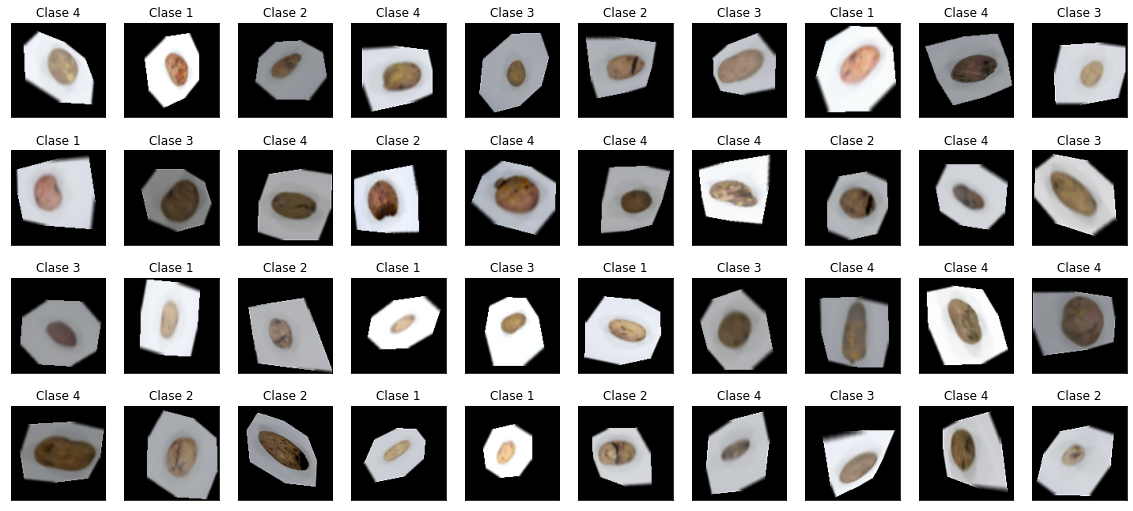
\includegraphics[scale=0.4]{Figs/augmentation.png}
	\caption{Matriz de Imágenes Con Transformaciones Aplicadas \\ Fuente: Elaboración Propia}
	\label{fig:agumentation}
\end{figure}	

\subsection{Funciones PotatoDataset y DataLoader}

Una vez se realiza el proceso de \textit{Data Augmentation}, se deben cargar las imágenes en \textit{Pytorch} para que puedan ser procesadas por el modelo de red neuronal. En esta sección se explica la creación de la función \textit{PotatoDataset()}, y la implementación de la función \textit{Dataloader}, ademas de la explicación de cada función, para cargar el conjunto de datos en \textit{Pytorch}.


\subsubsection{FUNCIÓN POTATODATASET}

Se creó una clase de \textit{Python} (\textit{Python Class Object Constructor}), con el nombre de \textit{AttributesDataset()}, que se encarga de leer el \textit{metadata}  de cada imágen y convertirlo en \textit{labelID}, en la Tabla \ref{table:metadata} se muestra como el algoritmo lee las imágenes dentro del modelo, sin embargo, las características deben ser ingresadas como \textit{labelID}, es decir, el \textit{label} Pastusa corresponde al ID $0$ en la categoría de Tipo. Este diccionario se presenta a continuación:			

\begin{itemize}
	\item Tipo: ${'Pastusa': 0, \ 'R12': 1}$
	\item Daño: ${'Buena': 0,\  'Defectuosa': 1}$
	\item Tamaño: ${'Muy Grande': 0,\ 'Grande': 1,\ 'Mediana': 2}$
\end{itemize}

En la red neuronal, únicamente se utilizaron \textit{labels} y \textit{labelID} de tipo y daño para definir las clases de la Tabla \ref{table:Clases}. La función \textit{Dataset} de \textit{Python} realiza el proceso de cargar y relacionar cada imágen con su respectivo \textit{label}, para \textit{Dataset's} que se encuentran organizados dentro de carpetas jerarquicamente. El \textit{Dataset} creado en éste documento no se encuentra organizado de esta manera, sino que la organización jerárquica que define las clases se encuentra dentro del \textit{metadata}, en el nombre de cada imágen, Tabla \ref{table:metadata}, debido a esto es que se desarrolló una función que cargara y relacionara de la misma manera que lo hace la función integrada de \textit{Pythorch}. Esta función fue llamada \textit{PotatoDataset()}, que utiliza los \textit{labelID} generados por la función \textit{AttributesDataset()}, y carga cada imágen relacionada con sus \textit{labelID}. Como se desarrolló la función, de igual forma debe ser capaz de aplicar las transformaciones a cada imágen. El objeto regresa las 592 imágenes cargadas en \textit{Python}, cada una relacionada con su respectivo \textit{labelID} y \textit{label}, y con una transformación o múltiples aplicadas. Esta función desarrollada, cuenta con los mismos atributos iterables que poseen los \textit{dataset's} creados a partir de la función integrada en \textit{Pytorch}.			


\subsubsection{FUNCIÓN DATALOADER}			

Generalmente, una vez se finaliza el proceso de cargar las imágenes utilizando la función \textit{DataSet} de \textit{Pytorch}, se procede a utilizar la función \textit{DataLoader} para generar múltiples lotes de imágenes, a partir de las transformaciones utilizadas. La función \textit{DataLoader()} de \textit{Pytorch}, es implementada para realizar la importación de datos a gran escala.\\
 
El \textit{dataset} que se generó a partir de la función creada \textit{PotatoDataset()} es del tipo \textit{iterable-style Datsets}, lo que permite utilizar la función integrada \textit{DataLoader()} de \textit{Pytorch}. La función permite la agrupación automática de muestras de datos individuales obtenidas en los lotes mediante argumentos. Los \textit{DataLoader's} cuentan con una gran cantidad de argumentos que permiten que la carga de datos sea más eficiente \cite{Pytorch}. Para la ejecución de la función se deben tener en cuenta los parámetros de la Tabla \ref{table:Argumentos}.

		
\begin{table}[ht]
	\centering
	\begin{tabular}{|p{2.5cm}|p{11cm}|}
		\hline
		FUNCIÓN & DESCRIPCIÓN \\ 
		\hline
		Batch size & Cuántas muestras por Batch hay que cargar (Default: 1)\\
		\hline
		Shuffle & Se establece en TRUE para que los datos se reorganicen en cada época (Default: FALSE)  \\
		\hline
		Num workers & Cuántos subprocesos se utilizarán para la carga de datos. 0 significa que los datos se cargarán en el proceso principal. (Default: 0)\\
		\hline
	\end{tabular}	
	\caption{Argumentos para el Dataloader}
	\label{table:Argumentos}
\end{table}

Los argumentos explicados en la tabla \ref{table:Argumentos} fueron establecidos de la siguiente forma:

\begin{itemize}
	\item $Batch \ Size = 40$
	\item $Shuffle = True$
	\item $Num \ workers = 0$
\end{itemize}

Esto con el objetivo de que el \textit{Dataloader} cargue 40 muestras por época, y tome otras 40 diferentes para la siguiente época, y así sucesivamente hasta terminar todas las épocas establecidas.  


\subsection{Hiperparámetros Del Modelo}

\subsubsection{FUNCIÓN DE PÉRDIDAS}		

\textit{Pytorch} posee una cantidad interesante de funciones de pérdidas para su uso en la clasificación de clases en redes neuronales. Una función de pérdidas, evalúa la desviación entre las predicciones realizadas por la red neuronal y los valores reales de las muestras utilizadas durante el entrenamiento de la red. La eficiencia de una red neuronal se mide en objeto a la función de pérdidas, cuanto menor sea el valor, es un indicativo que es más eficiente \cite{mathivet2018inteligencia}.\\
 	
Para el desarrollo de la red neuronal, se utilizó la pérdida de entropía cruzada entre la entrada y el objetivo. Es útil cuando se entrena un problema de clasificación con más de una clase. El objetivo que espera este criterio debe contener:

\begin{itemize}
	\item Índices de clase en el rango $[0,C)$ donde $C$ es el número de clases.
	\item Probabilidades de clase se requieren más allá de una sola clase cuando se encuentran etiquetas combinadas.				 
\end{itemize}

En cada lote usado en el entrenamiento de la red neuronal se encuentran etiquetas combinadas en el \textit{metadata} de las imágenes, como se describió en la Tabla \ref{table:Clases}, por lo tanto, una función de pérdida no reducida \cite{Pytorch} se describe en la Ecuación ~\ref{eq:perd}.\\

\begin{equation}
	\label{eq:perd}
	{l_n=-\sum_{c=1}^{C}w_c log\left(\frac{exp(x_n,c)}{\sum_{i=1}^{C}exp(x_n,i)}y_n,c\right)}
\end{equation}\\

Donde $x$ es la entrada, $y$ el objetivo de predicción, $w$ es el peso, $C$ el número de clases y $N$ es la dimensión del \textit{Batch}. Usando la función \textit{nn.CrossEntropyLoss()}, se calculan las pérdidas entre entrada y salida del modelo entrenado, para posteriormente utilizar estas pérdidas como métricas en porcentajes de \textit{Accuracy} y \textit{Losses}.\\			

El rendimiento de esta función de pérdidas es mejor cuando el objetivo contiene índices de clase y no las etiquetas, ya que esto permite optimizar el cálculo, por esta razón, se agruparon las etiquetas de las imágenes en $4 \ Clases$ definidas en la Tabla \ref{table:Clases}.

\subsubsection{OPTIMIZADOR}

\textit{Pytorch} posee el paquete \textit{torch.optim}, que implementa varios algoritmos de optimización derivados del \textit{gradiente descendiente}, definido por \textit{Sebastian Ruder (2016)} como "\textit{una forma de minimizar una función objetvio parametrizada por un modelo}" \cite{ruder2016overview}. A menudo se ha propuesto, por ejemplo \textit{Rumelhart (1986)} \cite{rumelhart1986learning}, minimizar el riesgo empírico  de una función objetivo $E_n(fw)$ utilizando el gradiente descendiente. Consiste en cada iteración actualizar los pesos $w$, como se muestra en la Ecuación \ref{eq:GD1}.

\begin{equation}
	\label{eq:GD1}
	{w_{i+1}=w_i-\gamma\frac{1}{n}\sum_{i=1}^{n}\nabla Q(z_i,w_t)}
\end{equation}\\

Donde $\gamma$ es la taza de aprendizaje elegida adecuadamente (\textit{learning rate}) y $\nabla Q(z,w)$ es la función de pérdidas evaluada en un punto y un peso $w$. Cuando la estimación inicial $w_0$ está lo suficientemente cerca del óptimo y cuando la tasa de aprendizaje es suficientemente pequeña, este algoritmo alcanza una convergencia lineal.\\

En el algoritmo desarrollado en este documento, se utilizó el optimizador de descenso estocástico del gradiente $SGD$, que es una simplificación drástica del algoritmo del gradiente descendiente. En lugar de calcular exactamente el gradiente de $E_n(fw)$, cada iteración estima este gradiente sobre la base de un único ejemplo $z_t$ elegido al azar \cite{bottou2012stochastic}.

\begin{equation}
	\label{eq:SGD1}
	{w_{i+1}=w_i-\gamma_t\nabla_w Q(z_t,w_t)}
\end{equation}

Se espera que la Ecuación~\ref{eq:GD1} se comporte como la Ecuación~\ref{eq:SGD1} a pesar del ruido introducido por este procedimiento simplificado. El algoritmo estocástico no necesita recordar qué ejemplos de datos fueron usados durante las iteraciones anteriores, por lo tanto, puede procesar ejemplos sobre la marcha en un sistema implementado. En esta situación, el descenso estocástico del gradiente optimiza directamente el riesgo esperado.	

\subsection{Arquitectura del modelo}

Se utilzaron modelos pre entrenados para realizar el entrenamiento del  \textit{dataset}, utilizando la teoría de \textit{Transfer Learning} que permite entrenar los modelos, con pesos establecidos entrenadas para otro tipo de datos, para obtener resultados a partir de ellos sin empezar desde cero la creación de una red neuronal y sus pesos. En este capítulo se presenta la estructura y los resultados obtenidos de los modelos pre entrenados \textit{AlexNet}, \textit{VGG19}, \textit{VGG11} y \textit{ResNet18}, sin el uso de un método de optimización de hiperparámetros.

\subsubsection{\MakeUppercase{Modelo preentrenado ALEXNET}}

El modelo \textit{AlexNet} fue implementado en el año $2012$ en el desafió de reconocimiento visual a gran escala \textit{ImageNet}. Este modelo tuvo un resultado tan satisfactorio, que los modelos de aprendizaje profundo, se convirtieron en la referencia para la investigación y desarrollo en los principales sectores de la industria \cite{krizhevsky2014one}\\


El modelo se compone de $5$ capas convolucionales y $3$ capas densas, donde las capas convolucionales están normalizadas por lotes de datos. El $kernel$ (Máscara aplicada en la convolución) tiene dimensiones diferentes que se distribuyen en \textit{11 x 11} en la primera capa, \textit{5 x 5} en la segunda y \textit{3 x 3} en las demás. La primera, cuarta y quinta capas convolucionales están conectadas por una capa \textit{Max pooling} con dimensiones de \textit{3 x 3}, que posee un \textit{stride} de $2$. Las capas convolucionales y de \textit{Max pooling} son seguidas por tres capas densas, en donde las primeras dos constan de $4096$ neuronas cada una y la última capa es la de salida, la cual se compone de $1000$ neuronas que poseen una función de activación \textit{softmax}, esta capa fue modificada para que sean $4$ neuronas de salida referentes a las 4 clases definidas para realizar la clasificación.

\begin{figure}[ht]
	\centering
	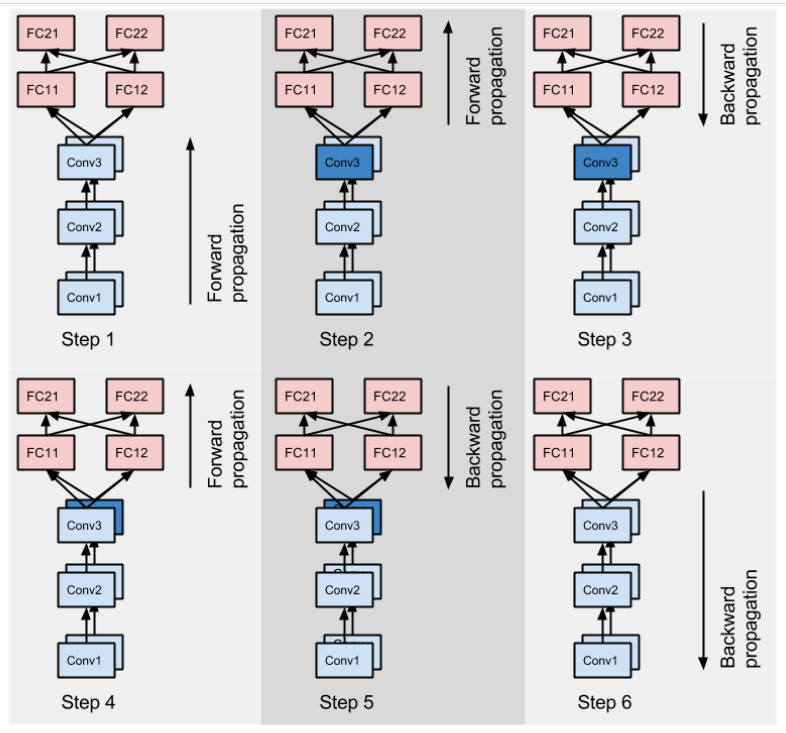
\includegraphics[scale=0.75]{Figs/5.png}
	\caption{Arquitectura Del Modelo \textit{AlexNet} \\ Fuente: Krizhevsky et al., (2012)}
	\label{fig:AlexNet}
\end{figure}

Como se aprecia en la Figura \ref{fig:AlexNet}, el modelo de \textit{AlexNet} toma una imagen de entrada con una resolución de \textit{224 x 224} píxeles y $3$ canales de color, la información recibida pasa por cinco capas convolucionales de neuronas con función de activación \textit{ReLu} y $3$ capas de \textit{Max pooling}. La quinta capa de convolución posee $256$ máscaras diferentes con dimensiones de \textit{13 x 13}. Se implementan las dos capas densas de $4096$ neuronas, las cuales están conectadas  por una capa de salida de $1000$ neuronas, que poseen una función de activación \textit{softmax}. Las neuronas presentes en la capa de salida representa una clase diferente \cite{alex}. Los resultados del entrenamiento obtenidos fueron inferiores al $20\%$, por lo tanto, fueron excluidos en el análisis sin optimización de los hiperparámetros.


\subsubsection{\MakeUppercase{Modelo preentrenado VGG19}}

La arquitectura \textit{VGG} fue planteada por Simonyan y Zisserman \cite{simonyan2014very},y es definida por Diaz-Gaxiola (2019) como ''grupos lineales de bloques que se encuentran formados por una cantidad determinada de capas convolucionales, una función de activación no lineal y una capa de \textit{Max pooling}, seguidos de tres capas densas y finalmente una capa de activación \textit{softmax}''. Esta arquitectura cuenta con $5$ bloques los cuales están distribuidos como se muestra en la Figura \ref{fig:VGG19}.				

\begin{figure}[ht]
	\centering
	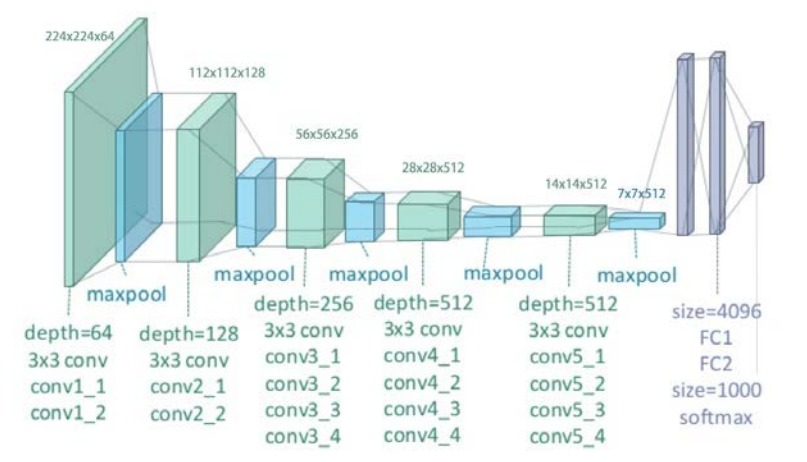
\includegraphics[scale=0.42]{Figs/22.jpeg}
	\caption{Arquitectura Del Modelo VGG \\ Fuente: Simonya, K. (2015)}
	\label{fig:VGG19}
\end{figure}			


Como se puede observar en la Figura \ref{fig:VGG19}, la columna \textit{E} muestra que la arquitectura del modelo \textit{VGG19}  cuenta con $2$ capas convolucionales de $64$ y $128$ filtros respectivamente, en sus dos primeros bloques, el bloque intermedio se compone de $3$ capas convolucionales de $256$ filtros, y los últimos dos bloques están compuestos por $3$ capas convolucionales de $512$ filtros cada uno. El numero $19$ representa la cantidad de capas que se pueden entrenar en la arquitectura, donde hay $16$ capas convolucionales y $3$ capas densas \cite{19}.\\			

Las capas convolucionales de esta arquitectura presentadas en la Figura \ref{fig:VGG19}, cuentan con un campo receptivo de \textit{3 x 3}, \textit{stride} de \textit{1 x 1} y \textit{padding} de $1$ pixel. Para realizar las operaciones de \textit{Max pooling} se tienen en cuenta un \textit{kernel} de dimensiones \textit{2 x 2}, \textit{stride} de \textit{2 x 2}, y por ultimo se implementa una función \textit{ReLu}. en cada capa oculta de la red para su activación. La Figura \ref{fig:VGG19_accuracy} muestra la precisión obtenida del entrenamiento hecho sobre esta arquitectura.

\begin{figure}[ht]
	\centering
	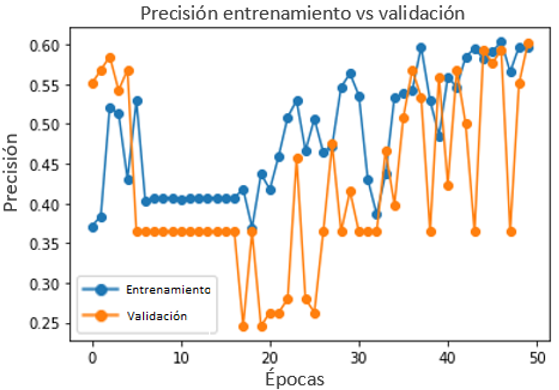
\includegraphics[scale=0.7]{Figs/101.png}
	\caption{Precisión Obtenida Con Modelo \textit{VGG19} \\ Fuente: Elaboración Propia}
	\label{fig:VGG19_accuracy}
\end{figure}  

\vspace{0.5cm}

La precisión del modelo al completar las $50$ épocas de entrenamiento es inferior al 60 \% como se observa en la Figura \ref{fig:VGG19_accuracy}. La figura \ref{fig:VGG19_losses} muestra el comportamiento de la función de pérdidas, que tiende a $0$ a medida que las épocas avanzan. La eficacia del modelo se mide a partir de que tan cercano a $0$ se obtiene la función de pérdidas. 

\newpage
\begin{figure}[ht]
	\centering
	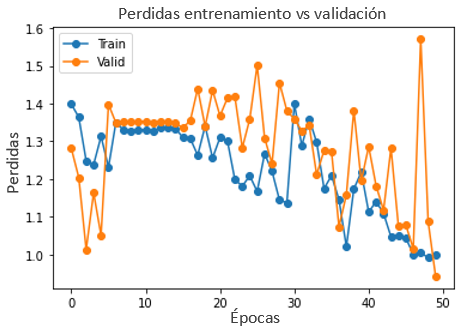
\includegraphics[scale=0.7]{Figs/102.png}
	\caption{Pérdidas Obtenidas Con Modelo \textit{VGG19} \\ Fuente: Elaboración Propia}
	\label{fig:VGG19_losses}
\end{figure}

\vspace{0.5cm}

El hecho de que en la última época, la precisión en el entrenamiento y en la validación dan valores similares, indica que el modelo no sufre de \textit{overfitting} que significaría un mal aprendizaje en la salida del modelo. Una vez se obtiene el modelo entrenado con los hiperparámetros no optimizados, se calcula la matriz de confusión con el conjunto de datos de \textit{validación}, los resultados se presentan en la Tabla \ref{fig:MC_VGG19}.

\vspace{0.5cm}

\begin{table}[htbp]
	\centering
	\resizebox{12cm}{!} {
	\begin{tabular}{|c|l|c|c|c|c|}
		\hline
		\multicolumn{2}{|c|}{\multirow{2}[4]{*}{}} & \multicolumn{4}{c|}{Predicción} \bigstrut\\
		\cline{3-6}    \multicolumn{2}{|c|}{} & CLASE 1 & CLASE 2 & CLASE 3 & CLASE 4 \bigstrut\\
		\hline
		\multirow{4}[8]{*}{\begin{sideways}Valor Real\end{sideways}} & CLASE 1 & 27     & 2     & 0    & 0 \bigstrut\\
		\cline{2-6}     & CLASE 2 & 21     & 1     & 0    & 2 \bigstrut\\
		\cline{2-6}      & CLASE 3 & 6     & 5     & 0    & 11 \bigstrut\\
		\cline{2-6}     & CLASE 4 & 20     & 15     & 0    & 8 \bigstrut\\
		\hline
	\end{tabular}
	}
	\caption{Matriz de confusión en conjunto de \textit{validación}}
	\label{fig:MC_VGG19}
\end{table}

\newpage

En la Tabla \ref{fig:ACU_VGG19} se presenta la precisión del modelo \textit{VGG 19} obtenida a partir de la matriz de confusión del conjunto de datos de \textit{validación} para cada una de las clases definidas.

\begin{table}[htbp]
	\centering
	\begin{tabular}{|c|c|}
		\hline
		CLASE 1 & 75,90 \bigstrut\\
		\hline
		CLASE 2 & 50,00 \bigstrut\\
		\hline
		CLASE 3 & 90,90 \bigstrut\\
		\hline
		CLASE 4 & 51,20 \bigstrut\\
		\hline
		\multicolumn{2}{|c|}{Precisión Total: 36,84} \bigstrut\\
		\hline
	\end{tabular}%
	\caption{Precisión por clase en conjunto de \textit{validación}}
	\label{fig:ACU_VGG19}
\end{table}%

Para comparar los resultados posteriormente, también se calcula la matriz de confusión con el conjunto de datos de \textit{entrenamiento}, los resultados se presentan en la Tabla \ref{fig:MC_VGG19_2}.

\begin{table}[htbp]
	\centering
	\resizebox{12cm}{!} {
		\begin{tabular}{|c|l|c|c|c|c|}
			\hline
			\multicolumn{2}{|c|}{\multirow{2}[4]{*}{}} & \multicolumn{4}{c|}{Predicción} \bigstrut\\
			\cline{3-6}    \multicolumn{2}{|c|}{} & CLASE 1 & CLASE 2 & CLASE 3 & CLASE 4 \bigstrut\\
			\hline
			\multirow{4}[8]{*}{\begin{sideways}Valor Real\end{sideways}} & CLASE 1 & 99     & 11     & 0    & 1 \bigstrut\\
			\cline{2-6}     & CLASE 2 & 64     & 22     & 0    & 0 \bigstrut\\
			\cline{2-6}      & CLASE 3 & 31     & 49     & 0    & 4 \bigstrut\\
			\cline{2-6}     & CLASE 4 & 84     & 103     & 0    & 6 \bigstrut\\
			\hline
		\end{tabular}
	}
	\caption{Matriz de confusión en conjunto de \textit{entrenamiento}}
	\label{fig:MC_VGG19_2}
\end{table}

En la Tabla \ref{fig:ACU_VGG19_2} se presenta la precisión del modelo obtenida a partir de la matriz de confusión del conjunto de datos de \textit{entrenamiento} para cada una de las clases definidas.

\begin{table}[htbp]
	\centering
	\begin{tabular}{|c|c|}
		\hline
		CLASE 1 & 89.20 \bigstrut\\
		\hline
		CLASE 2 & 25.60 \bigstrut\\
		\hline
		CLASE 3 & 0.00 \bigstrut\\
		\hline
		CLASE 4 & 3.10 \bigstrut\\
		\hline
		\multicolumn{2}{|c|}{Precisión Total: 26.47} \bigstrut\\
		\hline
	\end{tabular}%
	\caption{Precisión por clase en conjunto de \textit{entrenamiento}}
	\label{fig:ACU_VGG19_2}
\end{table}

\newpage
\subsubsection{\MakeUppercase{Modelo preentrenado VGG11}}

El modelo de aprendizaje profundo \textit{VGG11} es la configuración más sencilla de los modelos de arquitectura \textit{VGG}. Tiene 11 capas de peso en total, de ahí el nombre, 8 de ellas son capas convolucionales y 3 son capas completamente conectadas, como se aprecia en la Figura \ref{fig:VGG19} en la columna \textit{A}. Las 11 capas del modelo \textit{VGG11} son:
\begin{itemize}
	\item Convolución usando $64$ filtros + \textit{Max pooling}
	\item Convolución usando $128$ filtros + \textit{Max pooling}
	\item Convolución usando $256$ filtros
	\item Convolución usando $256$ filtros + \textit{Max pooling}
	\item Convolución usando filtros $512$
	\item Convolución usando $512$ filtros + \textit{Max pooling}
	\item Convolución usando filtros $512$
	\item Convolución usando $512$ filtros + \textit{Max pooling}
	\item Totalmente conectado con $4096$ neuronas
	\item Totalmente conectado con $4096$ neuronas
	\item Capa de salida con activación Softmax con $1000$ neuronas.
\end{itemize}

El modelo cuenta con $11$ capas ponderadas, sus pesos representan la fuerza de las conexiones entre unidades de capas de red adyacentes, son implementadas con el fin de conectar cada neurona de una capa con todas las neuronas de la siguiente capa, se debe tener en cuenta que la capa \textit{Max pooling} no se considera como una capa ponderada, debido a que es un mapa de características que contiene las características más destacadas. Los resultados del entrenamiento obtenidos fueron inferiores al $15\%$, por lo tanto, fueron excluidos en el análisis sin optimización de los hiperparámetros.

\subsubsection{\MakeUppercase{Modelo preentrenado RESNET18}}
La arquitectura \textit{ResNet} (Residual Net), fue propuesta por un equipo de Microsoft Research liderado por \textit{Kaiming He} \cite{he2016deep}, en donde se propone que si a una red neuronal de $20$ capas se le intercalan $36$ capas que calculan la simple función de identidad, la red resultante debería tener exactamente la misma eficacia y no ser inferior que la primera. Se debe recordar que la función identidad es la encargada de devolver exactamente el mismo valor que su argumento \cite{ref_4}. Para permitir que una red residual pueda variar su cantidad efectiva de capas, se introduce el concepto de bloque residual en la Figura \ref{fig:Bloque}.

\newpage
\begin{figure}[ht]
	\centering
	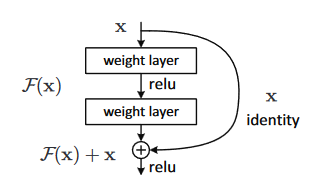
\includegraphics[scale=0.7]{Figs/67.png}
	\caption{Bloque Residual \\ Fuente: He, K. (2015) }
	\label{fig:Bloque}
\end{figure}

Como se aprecia en la Figura \ref{fig:Bloque}, el bloque residual se compone de una ruta residual, (izquierda), y una conexión atajo (derecha), que las une. La ruta residual $F(x)$, esta compuesta de dos capas de pesos sinápticos (pueden ser densas o convolucionales), que se intercalan por una función rectificadora. El resultado se suma con la información que atraviesa la conexión atajo \textit{X "identidad"}. Y por ultimo se aplica nuevamente la función rectificadora. La información puede atravesar con ello dos caminos diferentes que son: el de la función de identidad $X$ o el de la ruta residual \textit{F(x)} \cite{ref_5}.\\

En la arquitectura \textit{ResNet18}, las $18$ capas de esta arquitectura representan las 18 capas con pesos, en donde se incluye la capa de convolución y la capa totalmente conectada, excluyendo la capa de agrupación.

\begin{figure}[ht]
	\centering
	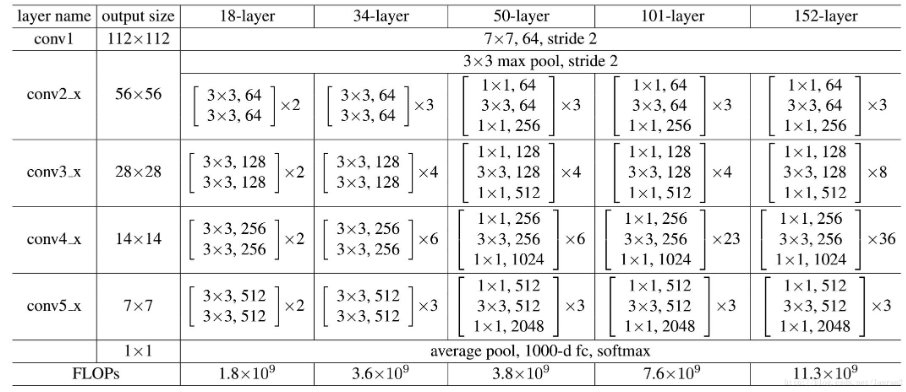
\includegraphics[scale=0.65]{Figs/68.png}
	\caption{Arquitectura \textit{ResNet18} \\ Fuente: He, K. (2015)}
	\label{fig:ArqRes18}
\end{figure}

Como se puede observar en la Figura \ref{fig:ArqRes18}, la primera capa de convolución implementa una máscara de \textit{7 x 77 x 7}, con un tamaño de paso de $2$ y un relleno de $3$. Luego, se aplican las capas con la función de activación \textit{ReLu} y \textit{Max pooling}. Estos constituyen la primera parte del modulo de convolución \textit{conv1}. Luego hay cuatro etapas, cada etapa tiene múltiples módulos, cada módulo se llama un bloque de construcción, por ende se evidencia que hay 8 bloques de construcción, como se presenta en la Figura \ref{fig:ArqRes18} \cite{ref_5}.\\				
	
La Figura \ref{fig:preci_RESNET18}, muestra la precisión obtenida en el entrenamiento del modelo \textit{ResNet18} durante $50$ épocas, sin haber aplicado la optimización bayesiana.

\vspace{0.5cm}

\begin{figure}[ht]
	\centering
	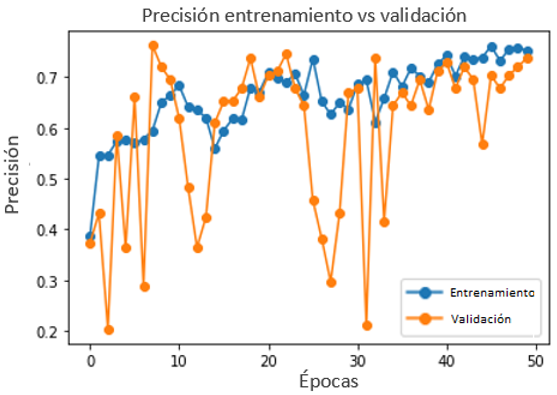
\includegraphics[scale=0.7]{Figs/109.png}
	\caption{Precisión Obtenida Con Modelo \textit{Resnet18} \\ Fuente: Elaboración Propia}
	\label{fig:preci_RESNET18}
\end{figure}


\vspace{0.5cm}

La información presentada en la Figura \ref{fig:preci_RESNET18} permite observar que el modelo obtuvo una precisión inferior al $80\%$ y, que el porcentaje de \textit{overfitting} se reduce en las épocas finales. La figura \ref{fig:perdda_RESNET18} muestra que la función de pérdidas tuvo un comportamiento con mayor eficacia en el entrenamiento con el modelo \textit{ResNet18}.

\newpage
\begin{figure}[ht]
	\centering
	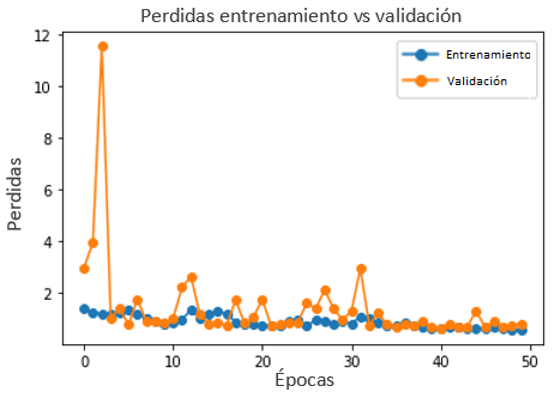
\includegraphics[scale=0.7]{Figs/110.png}
	\caption{Pérdidas Obtenidas Con Modelo \textit{Resnet18}\\ Fuente: Elaboración Propia}
	\label{fig:perdda_RESNET18}
\end{figure}

La matriz de confusión obtenida del modelo \textit{ResNet18} con el conjunto de datos de \textit{validación}, es presentada en la Tabla \ref*{MC_RESNET18}.\\

\begin{table}[htbp]
	\centering
	\resizebox{10cm}{!} {
	\begin{tabular}{|c|l|c|c|c|c|}
		\hline
		\multicolumn{2}{|c|}{\multirow{2}[4]{*}{}} & \multicolumn{4}{c|}{Predicción} \bigstrut\\
		\cline{3-6}    \multicolumn{2}{|c|}{} & CLASE 1 & CLASE 2 & CLASE 3 & CLASE 4 \bigstrut\\
		\hline
		\multirow{4}[8]{*}{\begin{sideways}Valor Real\end{sideways}} & CLASE 1 & 0     & 0     & 29    & 0 \bigstrut\\
		\cline{2-6}          & CLASE 2 & 0     & 0     & 24    & 0 \bigstrut\\
		\cline{2-6}          & CLASE 3 & 0     & 0     & 22    & 0 \bigstrut\\
		\cline{2-6}          & CLASE 4 & 0     & 0     & 43    & 0 \bigstrut\\
		\hline
	\end{tabular}%
	}
	\caption{Matriz de confusión en conjunto de \textit{validación}}
	\label{MC_RESNET18}
\end{table}

En la Tabla \ref*{clase_RESNET18}, se presenta la precisión del modelo aplicada al conjunto de datos de \textit{validación} por clases, obtenidas a partir de la matriz de confusión.

\newpage
\begin{table}[htbp]
	\centering
	\begin{tabular}{|c|c|}
		\hline
		CLASE 1 & 0,00 \bigstrut\\
		\hline
		CLASE 2 & 0,00 \bigstrut\\
		\hline
		CLASE 3 & 100,00 \bigstrut\\
		\hline
		CLASE 4 & 0,00 \bigstrut\\
		\hline
		\multicolumn{2}{|c|}{Precisión Total: 18,42} \bigstrut\\
		\hline
	\end{tabular}	
	\caption{Precisión por clase en conjunto de \textit{validación}}
	\label{clase_RESNET18}
\end{table}%


Para comparar los resultados posteriormente, se calcula la matriz de confusión con el conjunto de datos de \textit{entrenamiento}, los resultados se presentan en la Tabla \ref{MC_RESNET18_2}.

\begin{table}[htbp]
	\centering
	\resizebox{10cm}{!} {
		\begin{tabular}{|c|l|c|c|c|c|}
			\hline
			\multicolumn{2}{|c|}{\multirow{2}[4]{*}{}} & \multicolumn{4}{c|}{Predicción} \bigstrut\\
			\cline{3-6}    \multicolumn{2}{|c|}{} & CLASE 1 & CLASE 2 & CLASE 3 & CLASE 4 \bigstrut\\
			\hline
			\multirow{4}[8]{*}{\begin{sideways}Valor Real\end{sideways}} & CLASE 1 & 0     & 0     & 111    & 0 \bigstrut\\
			\cline{2-6}          & CLASE 2 & 0     & 0     & 86    & 0 \bigstrut\\
			\cline{2-6}          & CLASE 3 & 0     & 0     & 84    & 0 \bigstrut\\
			\cline{2-6}          & CLASE 4 & 0     & 0     & 193    & 0 \bigstrut\\
			\hline
		\end{tabular}%
	}
	\caption{Matriz de confusión en conjunto de \textit{entrenamiento}}
	\label{MC_RESNET18_2}
\end{table}%

En la Tabla \ref*{clase_RESNET18_2} se presenta la precisión del modelo aplicada al conjunto de datos de \textit{entrenamiento} por clases, obtenidas a partir de la matriz de confusión.

\begin{table}[htbp]
	\centering
	\begin{tabular}{|c|c|}
		\hline
		CLASE 1 & 0,00 \bigstrut\\
		\hline
		CLASE 2 & 0,00 \bigstrut\\
		\hline
		CLASE 3 & 100,00 \bigstrut\\
		\hline
		CLASE 4 & 0,00 \bigstrut\\
		\hline
		\multicolumn{2}{|c|}{Precisión Total: 23.52} \bigstrut\\
		\hline
	\end{tabular}%
	\caption{Precisión por clase en conjunto de \textit{entrenamiento}}
	\label{clase_RESNET18_2}
\end{table}%

\subsection{Optimización De Hiperparámetros}

La Tabla \ref{paraopt} muestra los hiperparámetros escogidos para optimizar utilizando la técnica de optimización Bayesiana. Estos hiperparámetros influyen en el comportamiento del optimizador, mejorando el proceso de aprendizaje de la \textit{RNC}.  

\begin{table}[ht]
	\centering
	\begin{tabular}{|c|c|c|ll}
		\cline{1-3}
		Parámetro & Limite inferior              & Limite Superior &  &  \\ \cline{1-3}
		Taza de Aprendizaje        & $1*10^{-6}$ & 0.4             &  &  \\ \cline{1-3}
		Momento   & 0                            & 1               &  &  \\ \cline{1-3}
		Tamaño del Paso   & 20                           & 40              &  &  \\ \cline{1-3}
	\end{tabular}
	\caption{Hiperparámetros Optimizados}
	\label{paraopt}
\end{table}

\textit{Botorch} realiza $20$ pruebas con parámetros distintos en los rangos definidos, y encuentra la combinación de parámetros que den el mejor resultado de precisión final del algoritmo. Estos resultados fueron utilizados para entrenar nuevamente los modelos descritos anteriormente, para comparar la eficacia de los algoritmos y modelos implementados.
	
\subsubsection{\MakeUppercase{Modelo AlexNet optimizado}}

En la Figura \ref{fig:preci_Alex_OPT}, se observa la precisión obtenida en el entrenamiento del modelo \textit{AlexNet} con hiperparámetros optimizados. A pesar de que la precisión es superior al $60\%$, que indica una mejora en los resultados con respecto a la versión no optimizada que no fueron tenidos en cuenta, se presenta un \textit{overfitting}, por lo que la red no está aprendiendo de manera correcta las características de el \textit{dataset}.

\begin{figure}[ht]
	\centering
	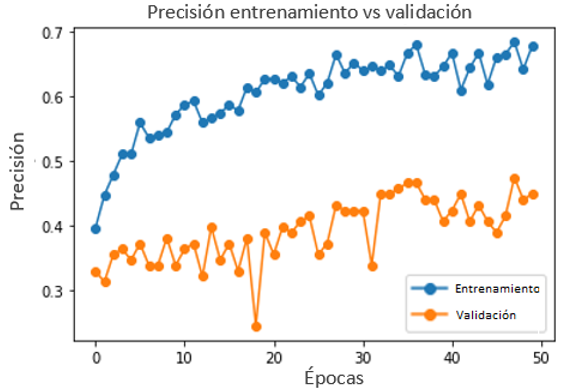
\includegraphics[scale=0.7]{Figs/500.png}
	\caption{Precisión modelo AlexNet optimizado\\ Fuente: Elaboración Propia}
	\label{fig:preci_Alex_OPT}
\end{figure}

\newpage
La Tabla \ref{tab:MC_ALEX_OPT} almacena los datos de la matriz de confusión del modelo \textit{AlexNet} optimizado en el conjunto de datos de \textit{validación}.

\begin{table}[htbp]
	\centering
	\resizebox{10cm}{!} {
	\begin{tabular}{|c|l|c|c|c|c|}
		\hline
		\multicolumn{2}{|c|}{\multirow{2}[4]{*}{}} & \multicolumn{4}{c|}{Predicción} \bigstrut\\
		\cline{3-6}    \multicolumn{2}{|c|}{} & CLASE 1 & CLASE 2 & CLASE 3 & CLASE 4 \bigstrut\\
		\hline
		\multirow{4}[8]{*}{\begin{sideways}Valor Real\end{sideways}} & CLASE 1 & 0     & 0     & 29    & 0 \bigstrut\\
		\cline{2-6}          & CLASE 2 & 0     & 1     & 22    & 1 \bigstrut\\
		\cline{2-6}          & CLASE 3 & 0     & 0     & 22    & 0 \bigstrut\\
		\cline{2-6}          & CLASE 4 & 0     & 1     & 42    & 0 \bigstrut\\
		\hline
	\end{tabular}
	}
	\caption{Matriz de confusión en conjunto de \textit{validación}}
	\label{tab:MC_ALEX_OPT}%
\end{table}%

La Tabla \ref{tab:Alexoptclases} presenta la precisión del modelo por cada clase en el conjunto de datos de \textit{validación}.


\begin{table}[htbp]
	\centering
	\begin{tabular}{|c|c|}
		\hline
		CLASE 1 & 0,00 \bigstrut\\
		\hline
		CLASE 2 & 4,20 \bigstrut\\
		\hline
		CLASE 3 & 100,00 \bigstrut\\
		\hline
		CLASE 4 & 0,00 \bigstrut\\
		\hline
		\multicolumn{2}{|c|}{Precisión Total: 21,05} \bigstrut\\
		\hline
	\end{tabular}%
	\caption{Clasificación por clase en conjunto de \textit{validación}
	}
	\label{tab:Alexoptclases}%
\end{table}%

La Tabla \ref{tab:MC_ALEX_OPT_2} almacena los datos de la matriz de confusión del modelo \textit{AlexNet} optimizado en el conjunto de datos de \textit{entrenamiento}.

\begin{table}[htbp]
	\centering
	\resizebox{10cm}{!} {
	\begin{tabular}{|c|l|c|c|c|c|}
		\hline
		\multicolumn{2}{|c|}{\multirow{2}[4]{*}{}} & \multicolumn{4}{c|}{Predicción} \bigstrut\\
		\cline{3-6}    \multicolumn{2}{|c|}{} & CLASE 1 & CLASE 2 & CLASE 3 & CLASE 4 \bigstrut\\
		\hline
		\multirow{4}[8]{*}{\begin{sideways}Valor Real\end{sideways}} & CLASE 1 & 0     & 0     & 111    & 0 \bigstrut\\
		\cline{2-6}          & CLASE 2 & 1     & 3     & 81    & 1 \bigstrut\\
		\cline{2-6}          & CLASE 3 & 0     & 0     & 84    & 0 \bigstrut\\
		\cline{2-6}          & CLASE 4 & 0     & 0     & 192    & 1 \bigstrut\\
		\hline
	\end{tabular}
	}
	\caption{Matriz de confusión en conjunto de \textit{entrenamiento}}
	\label{tab:MC_ALEX_OPT_2}%
\end{table}%

\newpage
La Tabla \ref{tab:Alexoptclases_2} presenta la precisión del modelo por cada clase en el conjunto de datos de \textit{entrenamiento}.

\begin{table}[htbp]
	\centering
	\begin{tabular}{|c|c|}
		\hline
		CLASE 1 & 0,00 \bigstrut\\
		\hline
		CLASE 2 & 3.50 \bigstrut\\
		\hline
		CLASE 3 & 100,00 \bigstrut\\
		\hline
		CLASE 4 & 0,50 \bigstrut\\
		\hline
		\multicolumn{2}{|c|}{Precisión Total: 14.70} \bigstrut\\
		\hline
	\end{tabular}%
	\caption{Clasificación por clase en conjunto de \textit{entrenamiento}
	}
	\label{tab:Alexoptclases_2}%
\end{table}%

A pesar de que la precisión en el entrenamiento del modelo superó el $60\%$ con los hiperparámetros optimizados, en la fase de validación del algoritmo, los resultados de precisión dieron una precisión del $14.7\%$, que indica el mal aprendizaje obtenido por la red representado en el \textit{overfitting} que presenta-

\subsubsection{\MakeUppercase{Modelo  VGG19 optimizado}}

La Figura \ref{fig:preci_vgg19_OPT}, muestra que la precisión obtenida en el entrenamiento del modelo \textit{VGG19} es de alrededor del $75 \%$ en validación, el cual es un valor que se acerca mucho al valor del modelo en entrenamiento de aproximadamente el $80 \%$.

\begin{figure}[ht]
	\centering
	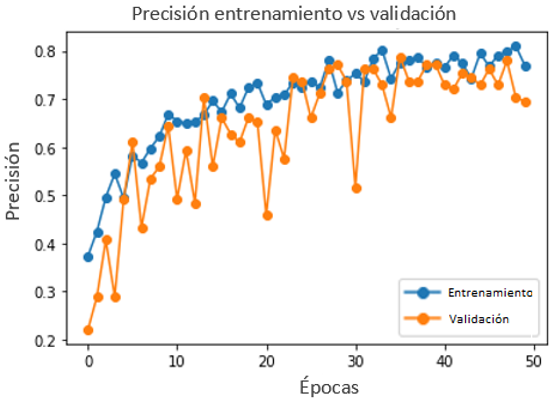
\includegraphics[scale=0.7]{Figs/504.png}
	\caption{Precisión modelo VGG-19 optimizado\\ Fuente: Elaboración Propia}
	\label{fig:preci_vgg19_OPT}
\end{figure}

\newpage
La Figura \ref{fig:perdda_vgg19_opt}, de igual forma, permite verificar el comportamiento de la función de pérdidas en el entrenamiento de este modelo, que indica una eficacia superior a los demás modelos entrenados debido al cercano valor a $0$ que presenta. 

\begin{figure}[ht]
	\centering
	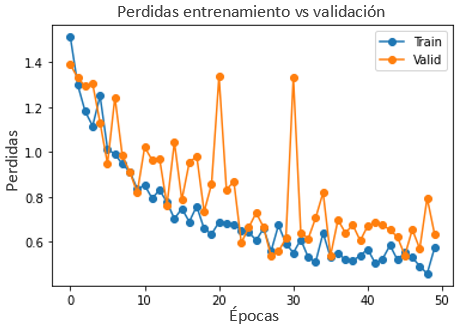
\includegraphics[scale=0.7]{Figs/505.png}
	\caption{Perdidas modelo VGG-19 optimizado \\ Fuente: Elaboración Propia}
	\label{fig:perdda_vgg19_opt}
\end{figure}

\vspace{0.5cm}

En la Tabla \ref{tab:MC_VGG19_OPT} se presenta la matriz de confusión obtenida del modelo \textit{VGG19} optimizado en el conjunto de datos de \textit{validación}.

\vspace{0.5cm}

\begin{table}[htbp]
	\centering
	\begin{tabular}{|c|l|c|c|c|c|}
		\hline
		\multicolumn{2}{|c|}{\multirow{2}[4]{*}{}} & \multicolumn{4}{c|}{Predicción} \bigstrut\\
		\cline{3-6}    \multicolumn{2}{|c|}{} & CLASE 1 & CLASE 2 & CLASE 3 & CLASE 4 \bigstrut\\
		\hline
		\multirow{4}[8]{*}{\begin{sideways}Valor Real\end{sideways}} & CLASE 1 & 22    & 0     & 7    & 0 \bigstrut\\
		\cline{2-6}          & CLASE 2 & 4     & 12     & 1    & 7 \bigstrut\\
		\cline{2-6}          & CLASE 3 & 1     & 0     & 20    & 1 \bigstrut\\
		\cline{2-6}          & CLASE 4 & 1     & 1     & 19    & 22 \bigstrut\\
		\hline
	\end{tabular}%
	\caption{Matriz de confusión en conjunto de \textit{validación}}
	\label{tab:MC_VGG19_OPT}%
\end{table}%


\newpage
La Tabla \ref{tab:VGG19optclases} presenta presenta la precisión del modelo por cada clase en el conjunto de datos de \textit{validación}.

\begin{table}[htbp]
	\centering
	\begin{tabular}{|c|c|}
		\hline
		CLASE 1 & 75,90 \bigstrut\\
		\hline
		CLASE 2 & 50,00 \bigstrut\\
		\hline
		CLASE 3 & 90,90 \bigstrut\\
		\hline
		CLASE 4 & 51,20 \bigstrut\\
		\hline
		\multicolumn{2}{|c|}{Precisión Total: 65,78} \bigstrut\\
		\hline
	\end{tabular}%
	\caption{Clasificación por clase en conjunto de \textit{validación}}
	\label{tab:VGG19optclases}%
\end{table}

La Tabla \ref{tab:MC_VGG19_OPT_2} almacena los datos de la matriz de confusión del modelo \textit{VGG19} optimizado en el conjunto de datos de \textit{entrenamiento}.

\begin{table}[htbp]
	\centering	
	\resizebox{10cm}{!} {
	\begin{tabular}{|c|l|c|c|c|c|}
		\hline
		\multicolumn{2}{|c|}{\multirow{2}[4]{*}{}} & \multicolumn{4}{c|}{Predicción} \bigstrut\\
		\cline{3-6}    \multicolumn{2}{|c|}{} & CLASE 1 & CLASE 2 & CLASE 3 & CLASE 4 \bigstrut\\
		\hline
		\multirow{4}[8]{*}{\begin{sideways}Valor Real\end{sideways}} & CLASE 1 & 80    & 0     & 31    & 0 \bigstrut\\
		\cline{2-6}          & CLASE 2 & 8     & 66     & 3    & 9 \bigstrut\\
		\cline{2-6}          & CLASE 3 & 1     & 0     & 83    & 0 \bigstrut\\
		\cline{2-6}          & CLASE 4 & 0     & 5     & 73    & 115 \bigstrut\\
		\hline
	\end{tabular}
	}
	\caption{Matriz de confusión en conjunto de \textit{entrenamiento}}
	\label{tab:MC_VGG19_OPT_2}%
\end{table}%

La Tabla \ref{tab:VGG19optclases_2} presenta la precisión del modelo por cada clase en el conjunto de datos de \textit{entrenamiento}.

\begin{table}[htbp]
	\centering
	\begin{tabular}{|c|c|}
		\hline
		CLASE 1 & 72.10 \bigstrut\\
		\hline
		CLASE 2 & 76.70 \bigstrut\\
		\hline
		CLASE 3 & 98.80 \bigstrut\\
		\hline
		CLASE 4 & 59.60 \bigstrut\\
		\hline
		\multicolumn{2}{|c|}{Precisión Total: 73.52} \bigstrut\\
		\hline
	\end{tabular}%
	\caption{Clasificación por clase en conjunto de \textit{entrenamiento}}
	\label{tab:VGG19optclases_2}%
\end{table}

\subsubsection{\MakeUppercase{Modelo VGG11 optimizado}}

La Figura \ref{fig:preci_vgg11_OPT} muestra observar la precisión obtenida en el entrenamiento del modelo \textit{VGG11} con parámetros optimizados. A pesar que la precisión es superior al $80\%$, lo cual es una mejora a los resultados obtenidos en los modelos anteriores, el entrenamiento tiene un porcentaje de \textit{overfitting} de aproximadamente $10\%$ que podría causar errores considerables en las predicciones.

\begin{figure}[ht]
	\centering
	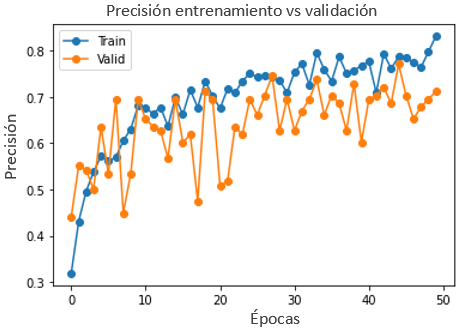
\includegraphics[scale=0.63]{Figs/508.png}
	\caption{Precisión modelo VGG11 optimizado\\Fuente: Elaboración Propia}
	\label{fig:preci_vgg11_OPT}
\end{figure}

La Figura \ref{fig:perdda_vgg11_opt} presenta las pérdidas del entrenamiento del modelo, a pesar que existe una clara desviación entre los datos predichos y los valores reales, las pérdidas indican valores inferiores a $1$, que indica que el entrenamiento no es totalmente ineficiente.

\begin{figure}[ht]
	\centering
	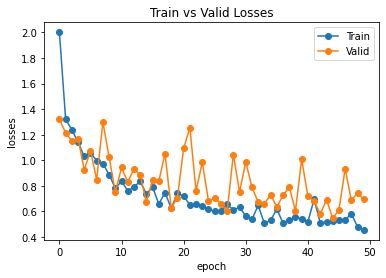
\includegraphics[scale=0.63]{Figs/509.png}
	\caption{Perdidas modelo VGG11 optimizado}
	\label{fig:perdda_vgg11_opt}
\end{figure}


\newpage
La Tabla \ref{tab:MC_VGG11_OPT},almacena los datos de la matriz de confusión del modelo \textit{VGG11} optimizado en el conjunto de datos de \textit{validación}.

\begin{table}[htbp]
	\centering
	\resizebox{11cm}{!} {
	\begin{tabular}{|c|l|c|c|c|c|}
		\hline
		\multicolumn{2}{|c|}{\multirow{2}[4]{*}{}} & \multicolumn{4}{c|}{Predicción} \bigstrut\\
		\cline{3-6}    \multicolumn{2}{|c|}{} & CLASE 1 & CLASE 2 & CLASE 3 & CLASE 4 \bigstrut\\
		\hline
		\multirow{4}[8]{*}{\begin{sideways}Valor Real\end{sideways}} & CLASE 1 & 18     & 0     & 11    & 0 \bigstrut\\
		\cline{2-6}          & CLASE 2 & 4     & 0     & 18    & 2 \bigstrut\\
		\cline{2-6}          & CLASE 3 & 2     & 0     & 20    & 0 \bigstrut\\
		\cline{2-6}          & CLASE 4 & 1     & 0     & 41    & 1 \bigstrut\\
		\hline
	\end{tabular}
	}
	\caption{Matriz de confusión en conjunto de \textit{validación}}
	\label{tab:MC_VGG11_OPT}%
\end{table}%

La Tabla \ref{tab:VGG11optclases} presenta la precisión del modelo por cada clase en el conjunto de datos de \textit{validación}.

\begin{table}[htbp]
	\centering
	\begin{tabular}{|c|c|}
		\hline
		CLASE 1 & 62,10 \bigstrut\\
		\hline
		CLASE 2 & 0,00 \bigstrut\\
		\hline
		CLASE 3 & 90,90 \bigstrut\\
		\hline
		CLASE 4 & 2,30 \bigstrut\\
		\hline
		\multicolumn{2}{|c|}{Precisión Total: 39,47} \bigstrut\\
		\hline
	\end{tabular}%
	\caption{Clasificación por clase en conjunto de \textit{validación}}
	\label{tab:VGG11optclases}%
\end{table}%

La Tabla \ref{tab:MC_VGG11_OPT_2} almacena los datos de la matriz de confusión del modelo \textit{VGG11} optimizado en el conjunto de datos de \textit{entrenamiento}.

\begin{table}[htbp]
	\centering
	\resizebox{11cm}{!} {
		\begin{tabular}{|c|l|c|c|c|c|}
			\hline
			\multicolumn{2}{|c|}{\multirow{2}[4]{*}{}} & \multicolumn{4}{c|}{Predicción} \bigstrut\\
			\cline{3-6}    \multicolumn{2}{|c|}{} & CLASE 1 & CLASE 2 & CLASE 3 & CLASE 4 \bigstrut\\
			\hline
			\multirow{4}[8]{*}{\begin{sideways}Valor Real\end{sideways}} & CLASE 1 & 69     & 0     & 42    & 0 \bigstrut\\
			\cline{2-6}          & CLASE 2 & 29     & 2     & 54    & 1 \bigstrut\\
			\cline{2-6}          & CLASE 3 & 2     & 0     & 82    & 0 \bigstrut\\
			\cline{2-6}          & CLASE 4 & 2     & 0     & 186    & 5 \bigstrut\\
			\hline
		\end{tabular}
	}
	\caption{Matriz de confusión en conjunto de \textit{entrenamiento}}
	\label{tab:MC_VGG11_OPT_2}%
\end{table}%

\newpage
La Tabla \ref{tab:VGG11optclases_2} presenta la precisión del modelo por cada clase en el conjunto de datos de \textit{entrenamiento}.

\begin{table}[htbp]
	\centering
	\begin{tabular}{|c|c|}
		\hline
		CLASE 1 & 62,20 \bigstrut\\
		\hline
		CLASE 2 & 2.30 \bigstrut\\
		\hline
		CLASE 3 & 97.60 \bigstrut\\
		\hline
		CLASE 4 & 2,60 \bigstrut\\
		\hline
		\multicolumn{2}{|c|}{Precisión Total: 40,35} \bigstrut\\
		\hline
	\end{tabular}%
	\caption{Clasificación por clase en conjunto de \textit{entrenamiento}}
	\label{tab:VGG11optclases_2}%
\end{table}%

\subsubsection{\MakeUppercase{Modelo ResNet18 Optimizado}}

La precisión obtenida en el entrenamiento del modelo \textit{ResNet18} se presenta en la Figura \ref{fig:preci_RES_OPT}, en donde se puede apreciar que el modelo presenta un alto porcentaje de \textit{overfitting}.

\begin{figure}[ht]
	\centering
	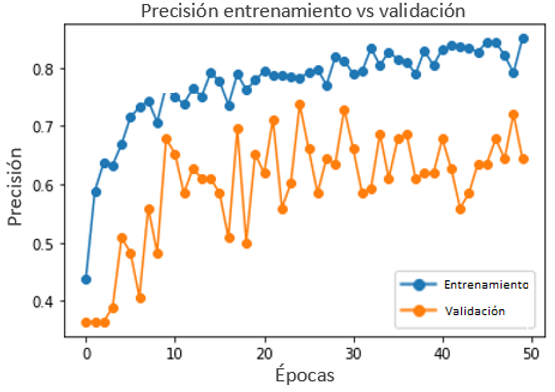
\includegraphics[scale=0.7]{Figs/512.png}
	\caption{Precisión modelo ResNet18 optimizado\\Fuente: Elaboración Propia}
	\label{fig:preci_RES_OPT}
\end{figure}

La Figura \ref{fig:perdda_REs_opt} muestra la tendencia del modelo a tener predicciones incorrectas e ineficiencia del entrenamiento debido al valor alto de pérdidas en la validación del modelo. 

\newpage
\begin{figure}[ht]
	\centering
	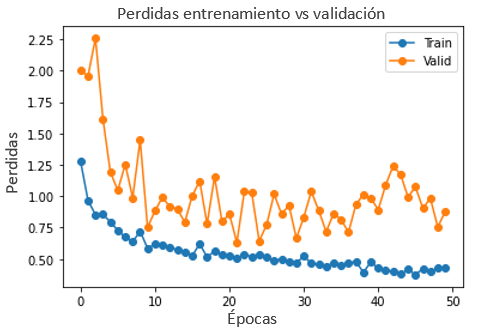
\includegraphics[scale=0.7]{Figs/513.png}
	\caption{Perdidas modelo ResNet18 optimizado\\Fuente: Elaboración Propia}
	\label{fig:perdda_REs_opt}
\end{figure}

\vspace{0.5cm}

En la Tabla \ref{tab:MC_resnet_OPT}, se puede evidenciar la matriz de confusión del modelo \textit{ResNet18} optimizado en el conjunto de datos de \textit{validación}.

\vspace{0.5cm}

\begin{table}[htbp]
	\centering
	\resizebox{13cm}{!} {
	\begin{tabular}{|c|l|c|c|c|c|}
		\hline
		\multicolumn{2}{|c|}{\multirow{2}[4]{*}{}} & \multicolumn{4}{c|}{Predicción} \bigstrut\\
		\cline{3-6}    \multicolumn{2}{|c|}{} & CLASE 1 & CLASE 2 & CLASE 3 & CLASE 4 \bigstrut\\
		\hline
		\multirow{4}[8]{*}{\begin{sideways}Valor Real\end{sideways}} & CLASE 1 & 29     & 0     & 0    & 0 \bigstrut\\
		\cline{2-6}          & CLASE 2 & 19     & 0     & 5    & 0 \bigstrut\\
		\cline{2-6}          & CLASE 3 & 12     & 0     & 10    & 0 \bigstrut\\
		\cline{2-6}          & CLASE 4 & 21     & 0     & 21    & 1 \bigstrut\\
		\hline
	\end{tabular}
	}
	\caption{Matriz de confusión en conjunto de \textit{validación}}
	\label{tab:MC_resnet_OPT}%
\end{table}

\newpage
La Tabla \ref{tab:resnetoptclases} presenta la precisión del modelo por cada clase en el conjunto de datos de \textit{validación}.

\begin{table}[htbp]
	\centering
	\begin{tabular}{|c|c|}
		\hline
		CLASE 1 & 100,00 \bigstrut\\
		\hline
		CLASE 2 & 0,00 \bigstrut\\
		\hline
		CLASE 3 & 45,50 \bigstrut\\
		\hline
		CLASE 4 & 2,30 \bigstrut\\
		\hline
		\multicolumn{2}{|c|}{Precisión Total: 36,84} \bigstrut\\
		\hline
	\end{tabular}%
	\caption{Clasificación por clase en conjunto de \textit{validación}}
	\label{tab:resnetoptclases}%
\end{table}

La Tabla \ref{tab:MC_resnet_OPT_2} almacena los datos de la matriz de confusión del modelo \textit{ResNet18} optimizado en el conjunto de datos de \textit{entrenamiento}.

\begin{table}[htbp]
	\centering
	\resizebox{10cm}{!} {
		\begin{tabular}{|c|l|c|c|c|c|}
			\hline
			\multicolumn{2}{|c|}{\multirow{2}[4]{*}{}} & \multicolumn{4}{c|}{Predicción} \bigstrut\\
			\cline{3-6}    \multicolumn{2}{|c|}{} & CLASE 1 & CLASE 2 & CLASE 3 & CLASE 4 \bigstrut\\
			\hline
			\multirow{4}[8]{*}{\begin{sideways}Valor Real\end{sideways}} & CLASE 1 & 110     & 0     & 1    & 0 \bigstrut\\
			\cline{2-6}          & CLASE 2 & 68     & 0     & 18    & 0 \bigstrut\\
			\cline{2-6}          & CLASE 3 & 47     & 0     & 37    & 0 \bigstrut\\
			\cline{2-6}          & CLASE 4 & 101     & 0     & 92    & 0 \bigstrut\\
			\hline
		\end{tabular}
	}
	\caption{Matriz de confusión en conjunto de \textit{entrenamiento}}
	\label{tab:MC_resnet_OPT_2}%
\end{table}

La Tabla \ref{tab:resnetoptclases_2} presenta la precisión del modelo por cada clase en el conjunto de datos de \textit{entrenamiento}.

\begin{table}[htbp]
	\centering
	\begin{tabular}{|c|c|}
		\hline
		CLASE 1 & 99,10 \bigstrut\\
		\hline
		CLASE 2 & 0,00 \bigstrut\\
		\hline
		CLASE 3 & 44,00 \bigstrut\\
		\hline
		CLASE 4 & 0,00 \bigstrut\\
		\hline
		\multicolumn{2}{|c|}{Precisión Total: 32,35} \bigstrut\\
		\hline
	\end{tabular}%
	\caption{Clasificación por clase en conjunto de \textit{entrenamiento}}
	\label{tab:resnetoptclases_2}%
\end{table}

\newpage		
\section{Clasificación Por Tamaño}

Para realizar la clasificación por tamaño se utilizó el módulo de visión artificial para \textit{Python} \textit{OpenCV}. Primero se realizó un estudio a un grupo de $5$ imágenes por cada uno de los tamaños. Se debe aplicar una umbralización para retirar el fondo de las imágenes, la Figura \ref{fig:matlabcv} muestra el uso de la herramienta de MATLAB\textsuperscript{\textregistered} \textit{Color Thresholder}.


\begin{figure}[ht]
	\centering
	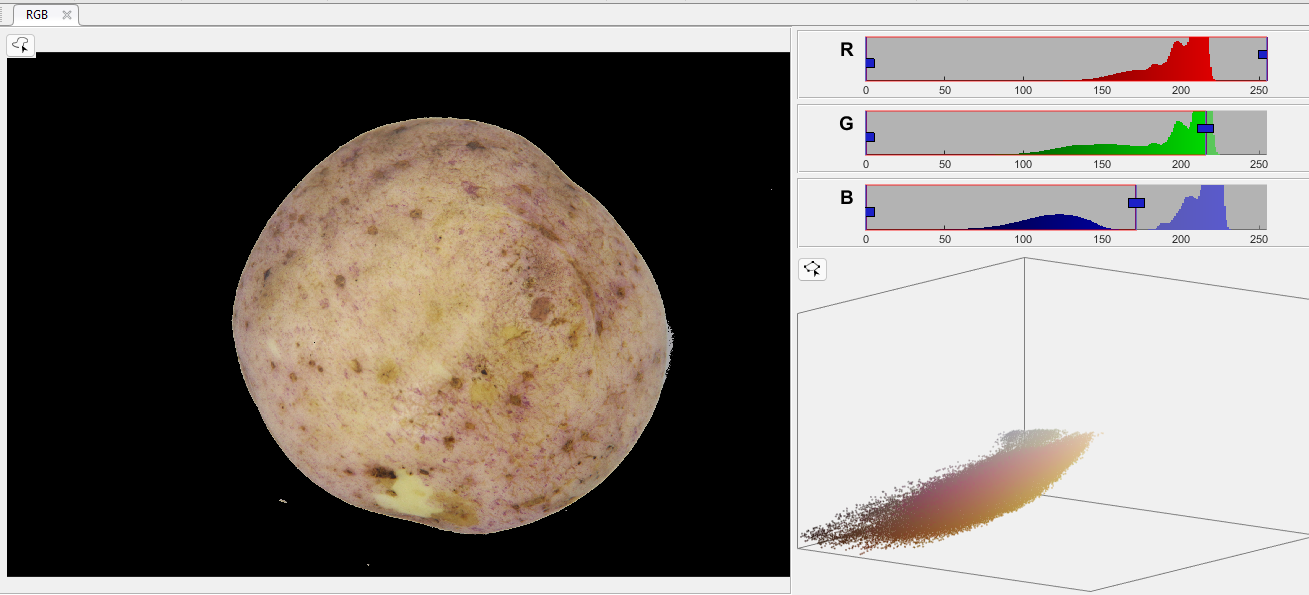
\includegraphics[scale=0.3]{Figs/matlabcv.png}
	\caption{Matlab Color Thresholder\\Fuente: Elaboración Propia}
	\label{fig:matlabcv}
\end{figure}

La herramienta permite, de forma interactiva, crear una función para quitar ciertos colores en el espacio \textit{RGB} de la imagén de muestra, en este caso, se realizó el proceso para retirar el fondo de la imagén de la papa, A este proceso se le conoce como umbralización. \\

Se pretende encontrar el perímetro aproximado de la papa utilizando la función \textit{FindContour} de\textit{OpenCV}, debido a esto, es necesario realizar una serie de transformaciones que conviertan la imágen de muestra, en una imágen binaria (blanco y negro). Se utilizaron los filtros de dilatación y mediana para realizar este proceso como se muestra en la Figura \ref{fig:dilmed}.	

\begin{figure}[ht]
	\centering
	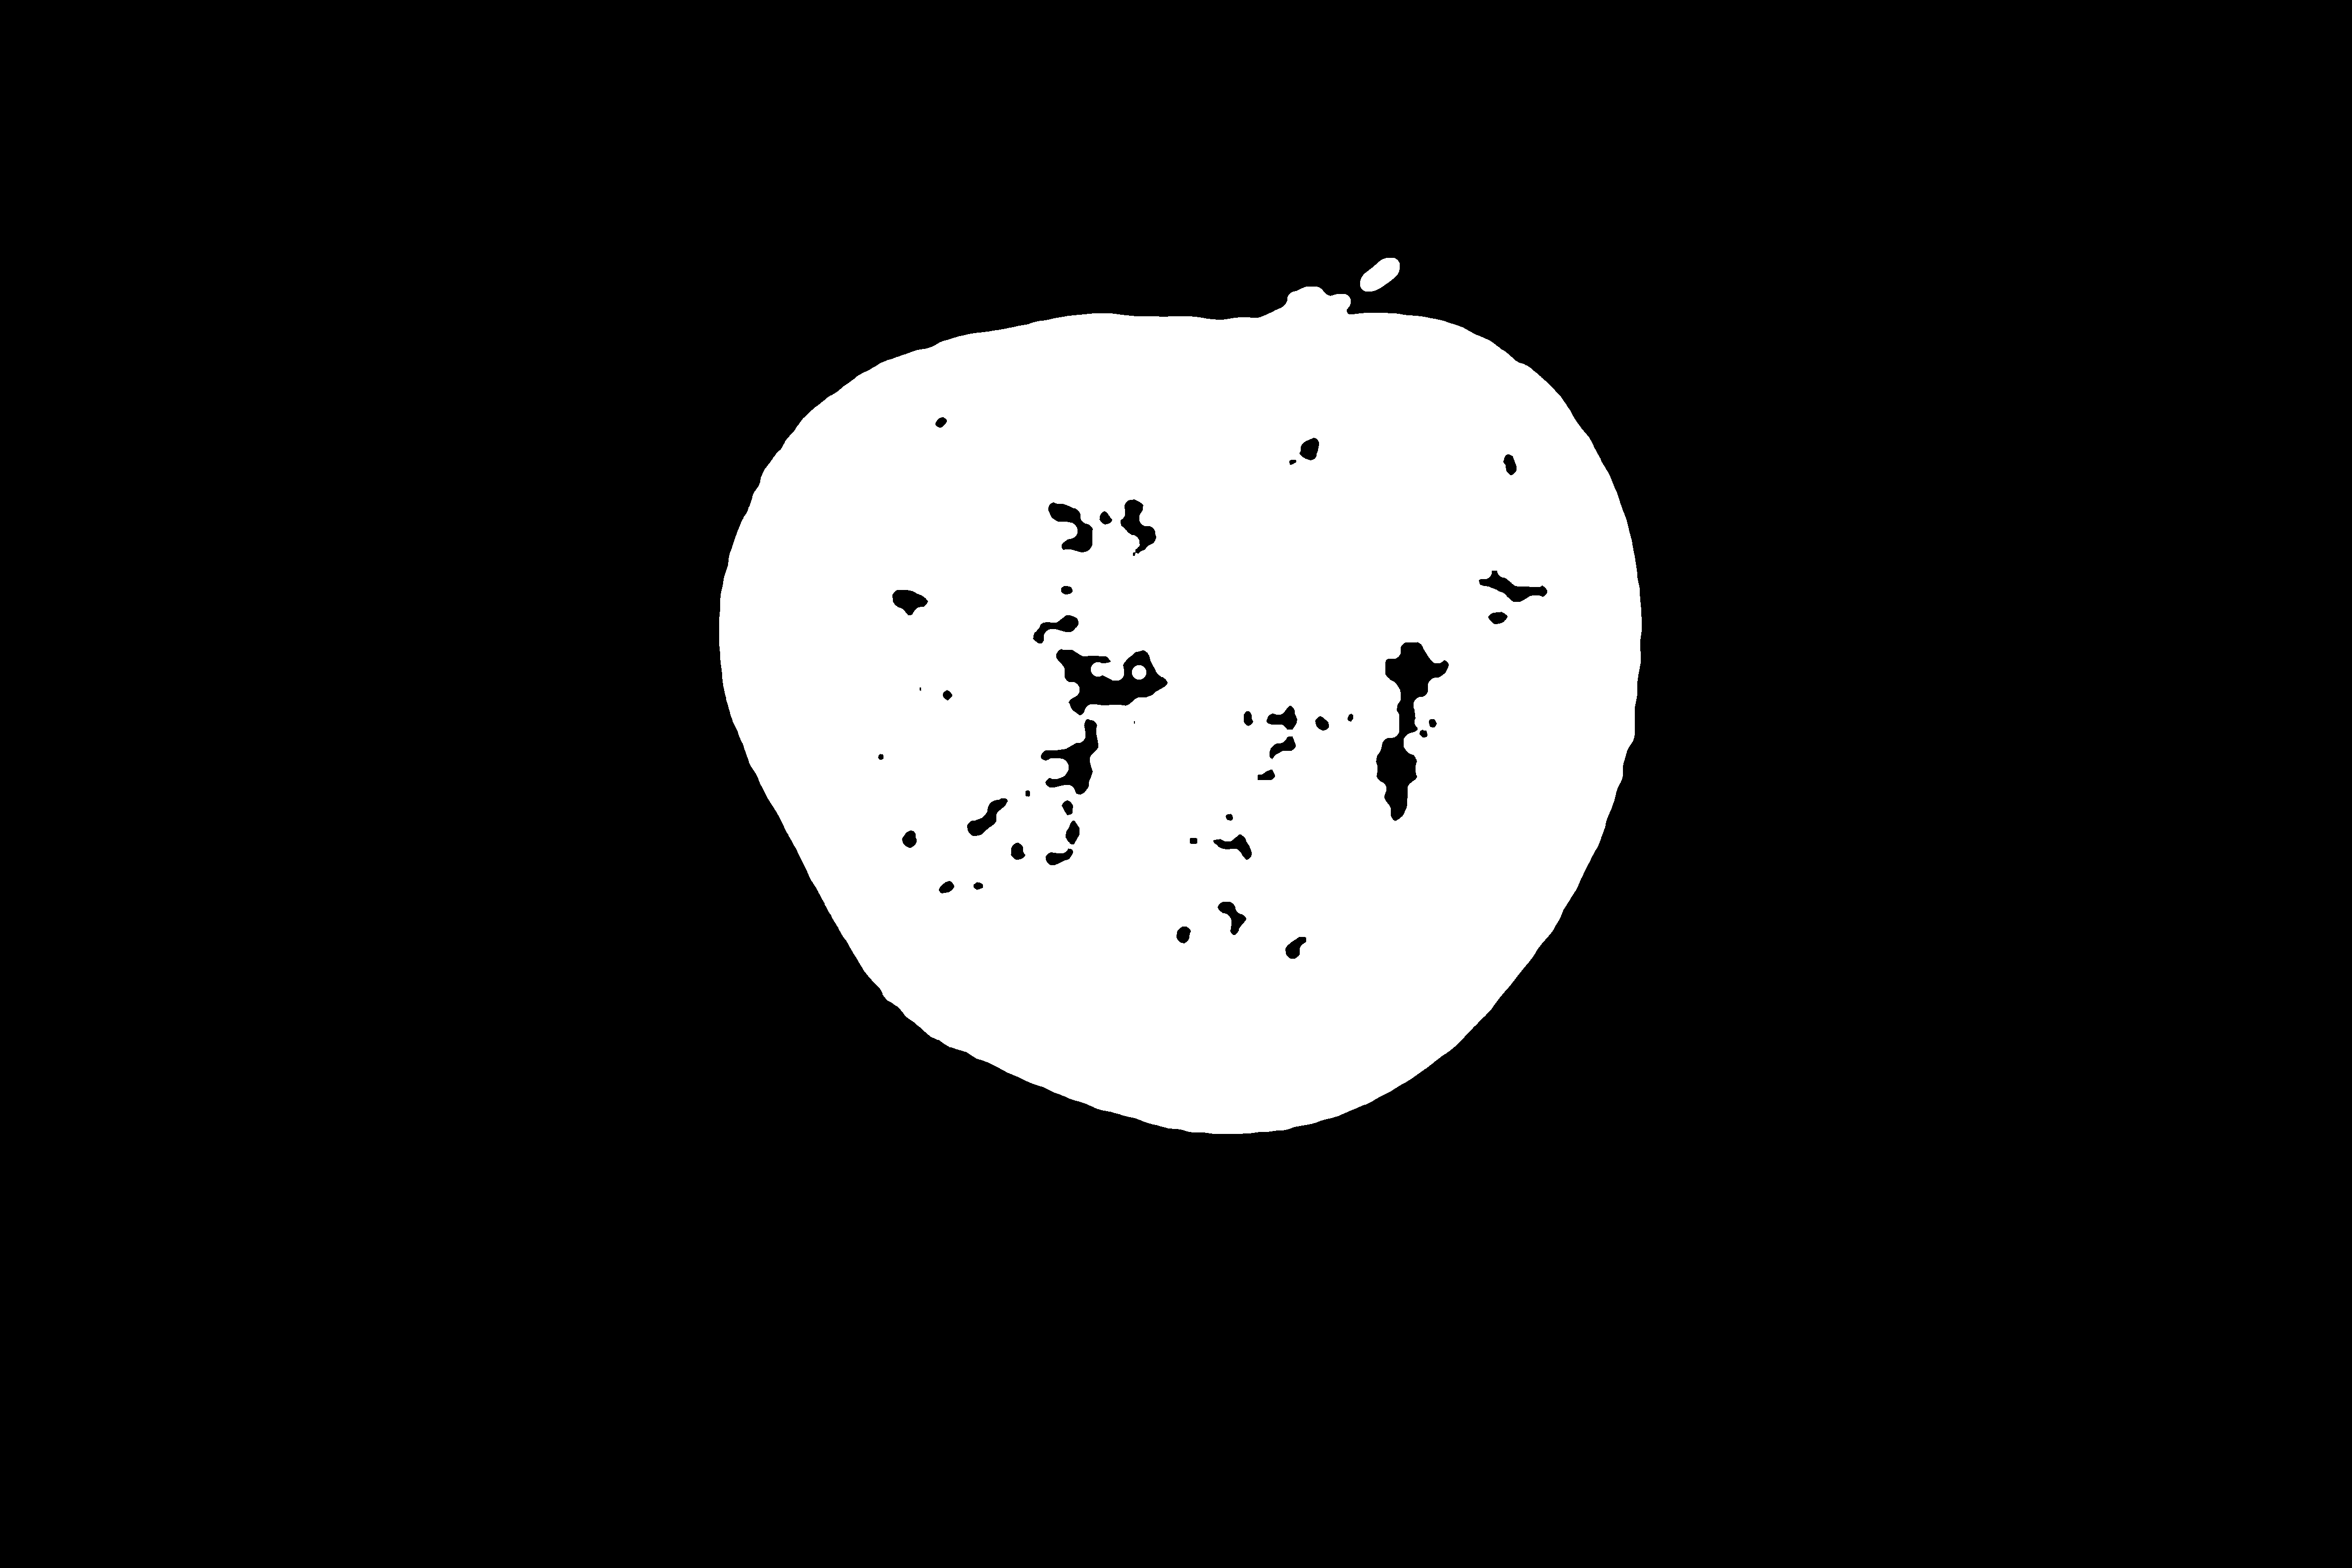
\includegraphics[scale=0.04]{Figs/dilmed.png}
	\caption{Imágen de Muestra Binarizada\\Fuente: Elaboración Propia}
	\label{fig:dilmed}
\end{figure}

\newpage
Con la imágen aislada de la mayoría de características que puedan interferir en el cálculo del perímetro, utilizando la función de \textit{FindContour}, se puede encontrar y dibujar un perímetro aproximado como se muestra en la Figura \ref{fig:contour}.

\begin{figure}[ht]
	\centering
	\includegraphics[scale=0.035]{Figs/contour.png}
	\caption{Perímetro Aproximado De Las Papas\\Fuente: Elaboración Propia}
	\label{fig:contour}
\end{figure}

En este punto, utilizando la función \textit{ArcLenght} de \textit{OpenCV}, se puede calcular el perímetro del contorno encontrado en cantidad de píxeles. Debido a que las imágenes tomadas para crear el \textit{dataset} fueron hechas desde una distancia fija desde el lente de la cámara, el tamaño relativo se puede asumir correcto en relación de tamaños. Se realizó un estudio en $5$ imágenes de cada tamaño, en donde se calcularon los perímetros, se calculó un promedio y una desviación estándar, para definir los límites en el tamaño de píxeles por cada tamaño de papa definido. En la Tabla \ref{table:perimetro} se muestran los resultados de estudio realizado.

\begin{table}[ht]
	\centering
	\resizebox{13cm}{!} {
	\begin{tabular}{cccccc}
		\hline
		\multicolumn{2}{|c|}{Muy Grande}                                                    & \multicolumn{2}{c|}{Grande}                                                        & \multicolumn{2}{c|}{Mediana}                                                       \\ \hline
		\multicolumn{1}{|c|}{Imagen}            & \multicolumn{1}{|p{2cm}|}{Tamaño del Perimetro} & \multicolumn{1}{c|}{Imagen}            & \multicolumn{1}{|p{2cm}|}{Tamaño del Perimetro} & \multicolumn{1}{c|}{Imagen}            & \multicolumn{1}{|p{2cm}|}{Tamaño del Perimetro} \\ \hline
		\multicolumn{1}{|c|}{0\_0\_0\_1963.jpg} & \multicolumn{1}{c|}{8580,08}              & \multicolumn{1}{c|}{0\_0\_1\_1239.jpg} & \multicolumn{1}{c|}{6524,93}          & \multicolumn{1}{c|}{0\_0\_2\_2011.jpg} & \multicolumn{1}{c|}{6074,97}          \\ \hline
		\multicolumn{1}{|c|}{0\_1\_0\_1806.jpg} & \multicolumn{1}{c|}{9523,78}              & \multicolumn{1}{c|}{0\_1\_1\_1828.jpg} & \multicolumn{1}{c|}{6802,54}          & \multicolumn{1}{c|}{0\_1\_2\_1506.jpg} & \multicolumn{1}{c|}{5018,00}                \\ \hline
		\multicolumn{1}{|c|}{1\_0\_0\_0777.jpg} & \multicolumn{1}{c|}{13275,00}               & \multicolumn{1}{c|}{1\_0\_1\_0796.jpg} & \multicolumn{1}{c|}{10602,79}          & \multicolumn{1}{c|}{1\_0\_2\_1995.jpg} & \multicolumn{1}{c|}{5090,17}          \\ \hline
		\multicolumn{1}{|c|}{1\_1\_0\_0825.jpg} & \multicolumn{1}{c|}{27830,00}               & \multicolumn{1}{c|}{1\_1\_1\_0770.jpg} & \multicolumn{1}{c|}{10285,33}          & \multicolumn{1}{c|}{1\_1\_2\_0857.jpg} & \multicolumn{1}{c|}{5500,75}          \\ \hline
		\multicolumn{1}{|c|}{0\_0\_0\_1964.jpg} & \multicolumn{1}{c|}{21607,00}               & \multicolumn{1}{c|}{0\_0\_1\_1240.jpg} & \multicolumn{1}{c|}{6726,00}                & \multicolumn{1}{c|}{0\_0\_2\_2013.jpg} & \multicolumn{1}{c|}{6046,62}          \\ \hline
		\multicolumn{1}{|c|}{Promedio}          & \multicolumn{1}{c|}{16163,19}             & \multicolumn{1}{c|}{Promedio}          & \multicolumn{1}{c|}{8188,33}              & \multicolumn{1}{c|}{Promedio}          & \multicolumn{1}{c|}{5546,12}              \\ \hline
		\multicolumn{1}{|c|}{Variacion STD}     & \multicolumn{1}{c|}{7425,23}          & \multicolumn{1}{c|}{Variacion STD}     & \multicolumn{1}{c|}{1846,76}          & \multicolumn{1}{c|}{Variacion STD}     & \multicolumn{1}{c|}{451,43}          \\ \hline
		\multicolumn{1}{|c|}{Limite inferior}   & \multicolumn{1}{c|}{9000,00}              & \multicolumn{1}{c|}{Limite inferior}   & \multicolumn{1}{c|}{6341,56}              & \multicolumn{1}{c|}{Limite inferior}   & \multicolumn{1}{c|}{5094,68}              \\ \hline
		\multicolumn{1}{|c|}{Limite superior}   & \multicolumn{1}{c|}{23588,42}             & \multicolumn{1}{c|}{Limite superior}   & \multicolumn{1}{c|}{9000,00}              & \multicolumn{1}{c|}{Limite superior}   & \multicolumn{1}{c|}{5997,56}              \\ \hline                           
	\end{tabular}
	}
	\caption{Perímetro en Tamaño de Píxeles}
	\label{table:perimetro}
\end{table}

De esta forma, se realiza la clasificación por tamaño en nuevas imágenes de papas, si el valor del perímetro se encuentra dentro de los límites inferior y superior calculados para cada tamaño, la imagen será clasificada de acuerdo a los rangos. Se obtuvo un $90\%$ de imágenes clasificadas correctamente en su tamaño en las imágenes del \textit{dataset}.

\section{Comparación De Precisión De Modelos Implementados}

En la Tabla \ref{table:compacon} se muestran los resultados obtenidos en la implementación de los $4$ modelos de \textit{RNC}.

\begin{table}[ht]
	\centering
	\resizebox{16cm}{!} {
		\begin{tabular}{|ccccc|ccccc|}
			\hline
			\multicolumn{5}{|c|}{Hiperparámetros Optimizados}                                                                                   & \multicolumn{5}{c|}{Hiperparámetros No Optimizados}                                                                                \\ \hline
			\multicolumn{5}{|c|}{Conjunto de Validación}                                                                                        & \multicolumn{5}{c|}{Conjunto de Validación}                                                                                        \\ \hline
			\multicolumn{1}{|c|}{Modelo}    & \multicolumn{1}{c|}{AlexNet} & \multicolumn{1}{c|}{VGG19} & \multicolumn{1}{c|}{VGG11} & ResNet18 & \multicolumn{1}{c|}{Modelo}    & \multicolumn{1}{c|}{AlexNet} & \multicolumn{1}{c|}{VGG19} & \multicolumn{1}{c|}{VGG11} & ResNet18 \\ \hline
			\multicolumn{1}{|c|}{Precisión[\%]} & \multicolumn{1}{c|}{$21,05$}   & \multicolumn{1}{c|}{$65,78$} & \multicolumn{1}{c|}{$39,47$} & $36,84$    & \multicolumn{1}{c|}{Precisión[\%]} & \multicolumn{1}{c|}{/}       & \multicolumn{1}{c|}{$36,84$} & \multicolumn{1}{c|}{/}     & $18,42$    \\ \hline
			\multicolumn{5}{|c|}{Conjunto de Entrenamiento}                                                                                     & \multicolumn{5}{c|}{Conjunto de Entrenamiento}                                                                                     \\ \hline
			\multicolumn{1}{|c|}{Modelo}    & \multicolumn{1}{c|}{AlexNet} & \multicolumn{1}{c|}{VGG19} & \multicolumn{1}{c|}{VGG11} & ResNet18 & \multicolumn{1}{c|}{Modelo}    & \multicolumn{1}{c|}{AlexNet} & \multicolumn{1}{c|}{VGG19} & \multicolumn{1}{c|}{VGG11} & ResNet18 \\ \hline
			\multicolumn{1}{|c|}{Precisión[\%]} & \multicolumn{1}{c|}{$14,70$}    & \multicolumn{1}{c|}{$73,52$} & \multicolumn{1}{c|}{$40,35$} & $32,35$    & \multicolumn{1}{c|}{Precisión[\%]} & \multicolumn{1}{c|}{/}       & \multicolumn{1}{c|}{$26,47$} & \multicolumn{1}{c|}{/}     & $23,52$    \\ \hline
		\end{tabular}
	}
	\caption{Precisión de los $4$ modelos implementados}
	\label{table:compacon}
\end{table}

Se observa que el modelo que obtuvo la mejor precisión fue con la arquitectura \textit{VGG19}, en donde se evidencia una mejora importante en los resultados al optimizar los hiperparámetros del modelo. La Figura \ref{fig:predvgg19} muestra una matriz con imágenes aleatorias del conjunto de \textit{entrenamiento}. En la parte superior de cada imágen se observa las siglas \textit{R.C} que corresponde a la clase real a la que pertenece, y la sigla \textit{Pred} que indica la predicción que realizó el modelo.

\begin{figure}[ht]
	\centering
	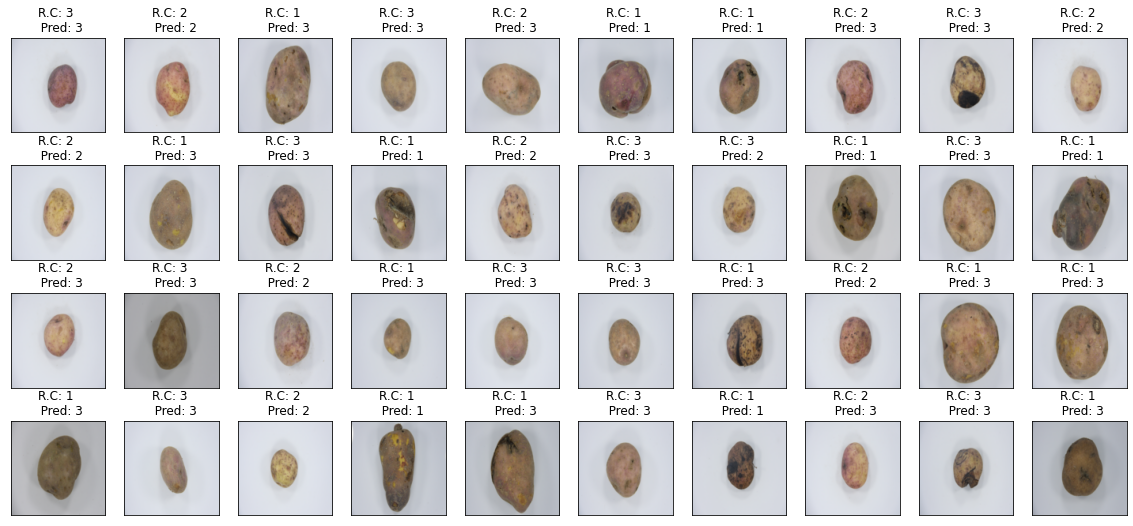
\includegraphics[scale=0.42]{Figs/506.png}
	\caption{Predicciones En El Conjunto De \textit{Entrenamiento} Del Modelo \textit{VGG19} \\ Fuente: Elaboración Propia}
	\label{fig:predvgg19}
\end{figure}

De esta forma se puede verificar que la optimización de hiperparámetros mejora considerablemente la eficiencia de una red neuronal, permitiendo que se obtengan mejores resultados en la fase de validación del algoritmo. \textit{Noordam, J}, en su trabajo obtuvo los resultados de la Tabla \ref{tab:noordam} en la clasificación de defectos en $5$ variedades de papa utilizando las técnicas de segmentación de color en imágenes  \textit{LDA} y \textit{MLF-NN}.

\begin{table}[ht]
	\centering
	\begin{tabular}{|c|c|c|}
		\hline
		Cultivo     & LDA(\%) & MLF-NN(\%) \\ \hline
		Bildstar    & 95,10   & 99,20      \\ \hline
		Bintje      & 96,20   & 96,20      \\ \hline
		Eigenheimer & 86,80   & 88,10      \\ \hline
		Irene       & 89,30   & 91,60       \\ \hline
		Sante       & 98,60    & 98,70       \\ \hline
	\end{tabular}
	\caption{Comparación entre \textit{MLF-NN} y \text{LDA} en $5$ variedades de papa \\ Fuente: Noordam, J. (2000)}
	\label{tab:noordam}
\end{table}

En la Figura \ref{fig:tabPAUL}, se muestran los resultados del sistema de clasificación de tamaño implementado por \textit{Paul, H} usando lel \textit{algoritmo de rastreo de 8 vecinos}. La clasificación obtuvo resultados de $96\%$ a $98\%$ para las muestras estáticas y de $77\%$ a $88\%$ en muestras en movimiento.

\begin{figure}[ht]
	\centering
	\includegraphics[scale=0.7]{Figs/tabPaul.png}
	\caption{Clasificación Por Tamaño Para Papas Estáticas y En Movimiento  \\ Fuente: Paul, H (1996)}
	\label{fig:tabPAUL}
\end{figure}

En los trabajos presentados por \textit{Paul, H} y \textit{Noordam, J} se observan resultados superiores (en términos de precisión de los algoritmos) a los obtenidos en el desarrollo de este proyecto, se evidencia que aplicando técnicas de segmentación de imágenes como \textit{LDA} y \textit{MLF-NN} previo a la implantación de la red neuronal ayuda a que el algoritmo generalice de mejor manera las imágenes, permitiendo que las predicciones tengan mayor precisión.\\


\newpage
\chapter{Prototipo}

\section{Especificaciones principales}
Se implementa una banda transportadora, tomada de una maquina selladora de banda continua horizontal FR-900, la cual es impulsada por un motor DC a 220V. Las especificaciones técnicas de la selladora, se presentan en la Tabla \ref{fig:principales}. La máquina se alimenta con $220 \ VAC$ a $50 \ HZ$ y su estructura es en acero inoxidable. 

\begin{table}[ht]
	\centering
	\begin{tabular}{|c|c|c|c|}
		\hline
		\multicolumn{4}{|l|}{\textbf{MOTOR}} \bigstrut\\
		\hline
		\multicolumn{2}{|c|}{REFERENCIA:} & \multicolumn{2}{c|}{ZYT 90-01} \bigstrut\\
		\hline
		\multicolumn{2}{|c|}{CORRIENTE:} & \multicolumn{2}{c|}{0,32 A} \bigstrut\\
		\hline
		\multicolumn{2}{|c|}{VOLTAJE:} & \multicolumn{2}{c|}{220 VDC} \bigstrut\\
		\hline
		\multicolumn{2}{|c|}{VELOCIDAD:} & \multicolumn{2}{c|}{2000 r/min} \bigstrut\\
		\hline
		\multicolumn{2}{|c|}{POTENCIA:} & \multicolumn{2}{c|}{50 W} \bigstrut\\
		\hline
		\multicolumn{4}{|l|}{\textbf{DIMENSIONES}} \bigstrut\\
		\hline
		\multicolumn{2}{|c|}{HORIZONTAL:} & \multicolumn{2}{c|}{850 x 420 x 320 (mm)} \bigstrut\\
		\hline
		\multicolumn{2}{|c|}{VERTICAL:} & \multicolumn{2}{c|}{850 x 320 x 550 (mm)} \bigstrut\\
		\hline
		\multicolumn{2}{|c|}{CONSOLA:} & \multicolumn{2}{c|}{850 x 320 x 1000 (mm)} \bigstrut\\
		\hline
	\end{tabular}%
	\caption{Especificaciones Principales}
	\label{fig:principales}
\end{table}%


\newpage
\section{Descripción de la maquina}
En la Figura \ref{fig:Banda}, se presenta un esquema general de la maquina selladora de banda continua horizontal FR-900, y en la Tabla \ref{table:Banda} se describen las partes presentadas en la Figura \ref{fig:Banda}.
\begin{figure}[ht]
	\centering
	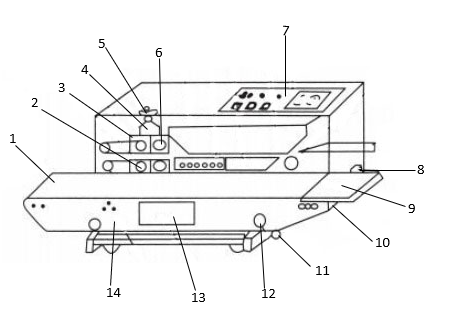
\includegraphics[scale=0.95]{Figs/65.png}
	\caption{Maquina Banda Transportadora}
	\label{fig:Banda}
\end{figure}

\begin{table}[ht]
	\centering
	\begin{tabular}{|p{5cm}|p{8cm}|}
		\hline
		1- Cinta transportadora & 8- Enchufe de corriente y protección \\ 
		\hline
		2- Rueda de goma& 9- Mesa de trabajo fija\\
		\hline
		3- Rodillo de goma& 10- Tornillo de regulación de la elasticidad de las cintas transportadoras\\
		\hline
		4- Asiento rueda de tintorería& 11- Perilla de regulación de la entrada y salida de la estación de transporte\\
		\hline
		5- Rueda reguladora de presión& 12- Perilla de regulación de la altura de la estación transportadora\\
		\hline
		6- Rueda motriz& 13- Placa de identificación\\
		\hline
		7- Caja de Control& 14- Estación de transporte\\
		\hline
	\end{tabular}	
	\caption{Descripción Maquina Transportadora}
	\label{table:Banda}
\end{table}

\newpage
\section{Esquema eléctrico}
En la Figura \ref{fig:Esquema} se presenta las conexiones eléctricas realizadas para el funcionamiento del prototipo, ademas de esto, se anexa en la Tabla \ref{table:esquema} el listado de elementos implementados.  
\begin{figure}[ht]
	\centering
	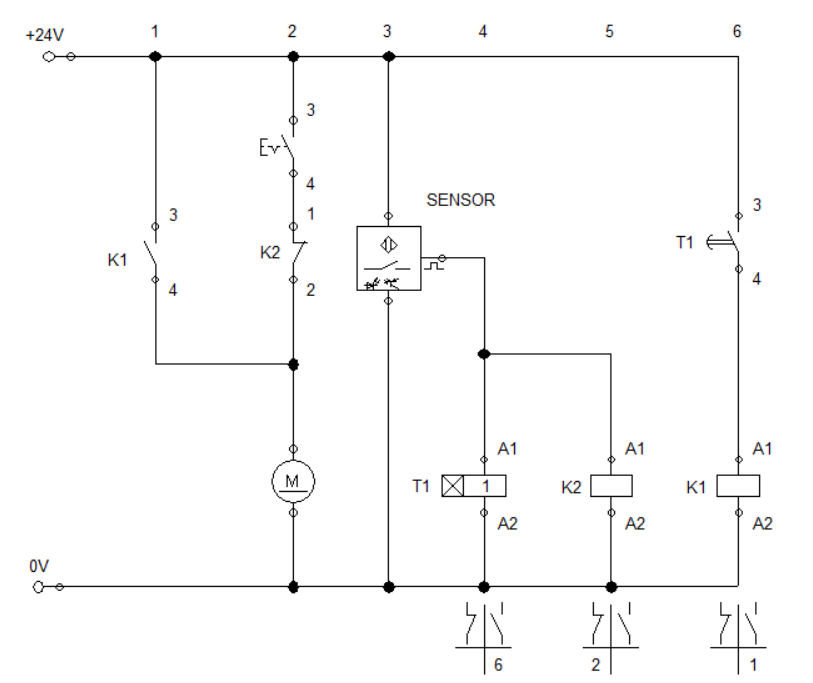
\includegraphics[scale=0.5]{Figs/66.png}
	\caption{Esquema eléctrico}
	\label{fig:Esquema}
\end{figure}

\begin{table}[ht]
	\centering
	\begin{tabular}{|p{2cm}|p{5cm}|p{3cm}|}
		\hline
		SÍMBOLO & NOMBRE & CANTIDAD \\ 
		\hline
		V1 & Fuente de Voltaje & 1 \\
		\hline
		T1 & Temporizador & 1 \\
		\hline
		K1 & Relé & 1 \\
		\hline
		M1 & Motor DC & 1 \\
		\hline
		SENSOR & Sensor Fotoeléctrico & 1 \\
		\hline
		K2 & Relé & 1 \\
		\hline
	\end{tabular}	
	\caption{Elementos Esquema Eléctrico}
	\label{table:esquema}
\end{table}	

\newpage	
\section{Estructura}
La caja elaborada para el análisis de los tubérculos de papas, fue construida en acetato con medidas de, \textit{35 x 25(cm)} las laminas frontal y trasera (Figuras \ref{fig:frontal} y \ref{fig:trasera}), \textit{16 x 25(cm)} lamina superior (Figura \ref{fig:superior}), \textit{20 x 16(cm)} laminas laterales como se muestra en la Figura \ref{fig:lateral}.

\begin{figure}[h!]
	\centering
	\begin{subfigure}{0.45\linewidth}
		\centering
		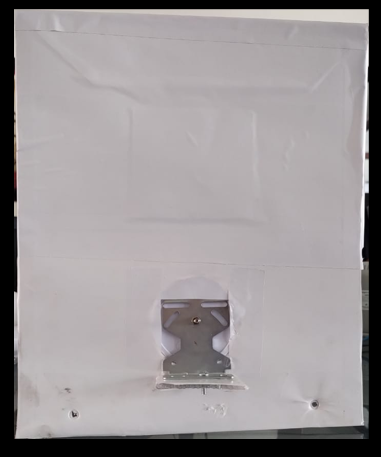
\includegraphics[scale=0.3]{Figs/300.png}
		\caption{Lamina Frontal}
		\label{fig:frontal}
	\end{subfigure}
	\begin{subfigure}{0.45\linewidth}
		\centering
		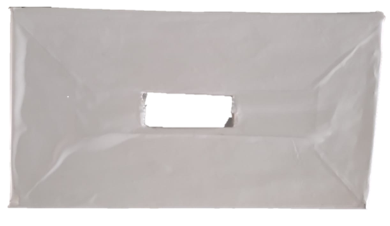
\includegraphics[scale=0.5]{Figs/301.png}
		\caption{Lamina superior}
		\label{fig:superior}
	\end{subfigure}
	\caption{Estructura de Análisis Laminas Principales}
	\label{fig:estructura}
\end{figure} 

\begin{figure}[h!]
	\centering
	\begin{subfigure}{0.45\linewidth}
		\centering
		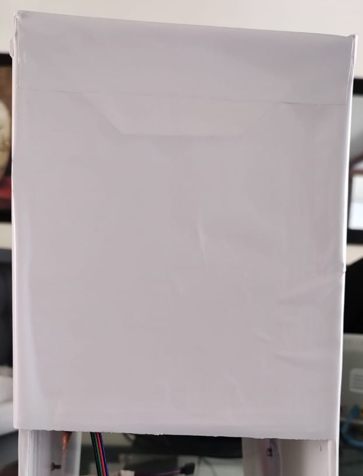
\includegraphics[scale=0.3]{Figs/302.png}
		\caption{Lamina lateral}
		\label{fig:lateral}
	\end{subfigure}
	\begin{subfigure}{0.45\linewidth}
		\centering
		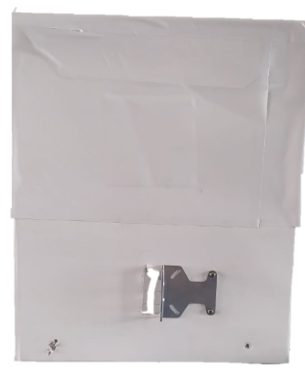
\includegraphics[scale=0.3]{Figs/303.png}
		\caption{Lamina Trasera}
		\label{fig:trasera}
	\end{subfigure}
	\caption{Estructura de Análisis Laminas Laterales}
	\label{fig:estructura}
\end{figure} 


Como se muestra en las Figuras , las laminas fueron diseñadas con las medidas necesarias para posicionar algunos elementos, que permitieran realizar la clasificación de los tuberculos, como lo son bombillos, un sensor optico y una camara web, los cuales seran definidos en los numerales \textit{6.4.1, 6.4.2 y 6.4.3}.

\subsection{Bombillos}
La estructura cuenta con dos agujeros, donde se ubican dos bombillos de luz blanca de 6500 Kelvin de temperatura, para mantener la iluminación fija, a una distancia de 30 cm de todas las fotos, al igual que se tomaron durante la construcción del Dataset.
\subsection{Sensor Fotoeléctrico}
Se implementa un sensor fotoeléctrico, de referencia MAGEWAY, el cual tiene como objetivo detener la banda transportadora una vez el tubérculo de papa se encuentre posicionado bajo la cámara, para realizar su respectiva inspección, el sensor cuenta con las siguientes especificaciones.
\\
\\
\textbf{ESPECIFICACIONES TÉCNICAS:}
\begin{itemize}
	\item Método de detección: retroreflectante.
	\item Ángulo: 1,5 o aprox.
	\item Máx. Rango de detección: 4 m.
	\item Voltaje de alimentación: 12-240 VDC, 24-240V ACBR, Salida: Relé SPDT
	\item Capacidad de salida: 3 A/30 VCC, 3 A/250 VAC.
	\item Temperatura ambiente: -4-131 °F (-20-55 °C).
\end{itemize}

\subsection{Cámara Web}
Para la detección de los tubérculos de papa, se implementa una cámara \textit{Web Camera America Store}, la cual será la encargada de la toma de fotos de los tubérculos, mientras son transportados en la banda transportadora para su análisis.
\\
\\
\textbf{ESPECIFICACIONES TÉCNICAS:}
\begin{itemize}
	\item Lente: Lente de Cristal
	\item Tamaño del artículo: 8 x 4 x 8 cm
	\item Chip DSP: sin controlador
	\item Sensor de imagen: CMOS
	\item Resolución dinámica: 1920 x 1080
	\item Marco: 30 fps
	\item Longitud Focal: 8 mm - infinity
	\item Longitud del Cable: aproximadamente 138 cm
\end{itemize}

\section{Funcionamiento}
Aquí se describe el funcionamiento mecánico de la maquina y el funcionamiento de la red neuronal, la cual fue programada en la tarjeta Jetson Nano para realizar la clasificación de los tubérculos de papa.

\subsection{Funcionamiento Mecánico}
El funcionamiento mecánico inicia conectando la alimentación de la maquina, una vez la maquina se encuentre conectada, el indicador luminoso que se encuentra en el pulsador de inicio, se activará, como se muestra en la Figura \ref{fig:indicador}, esto para dar a conocer que la maquina ya puede entrar en funcionamiento.

\begin{figure}[ht]
	\centering
	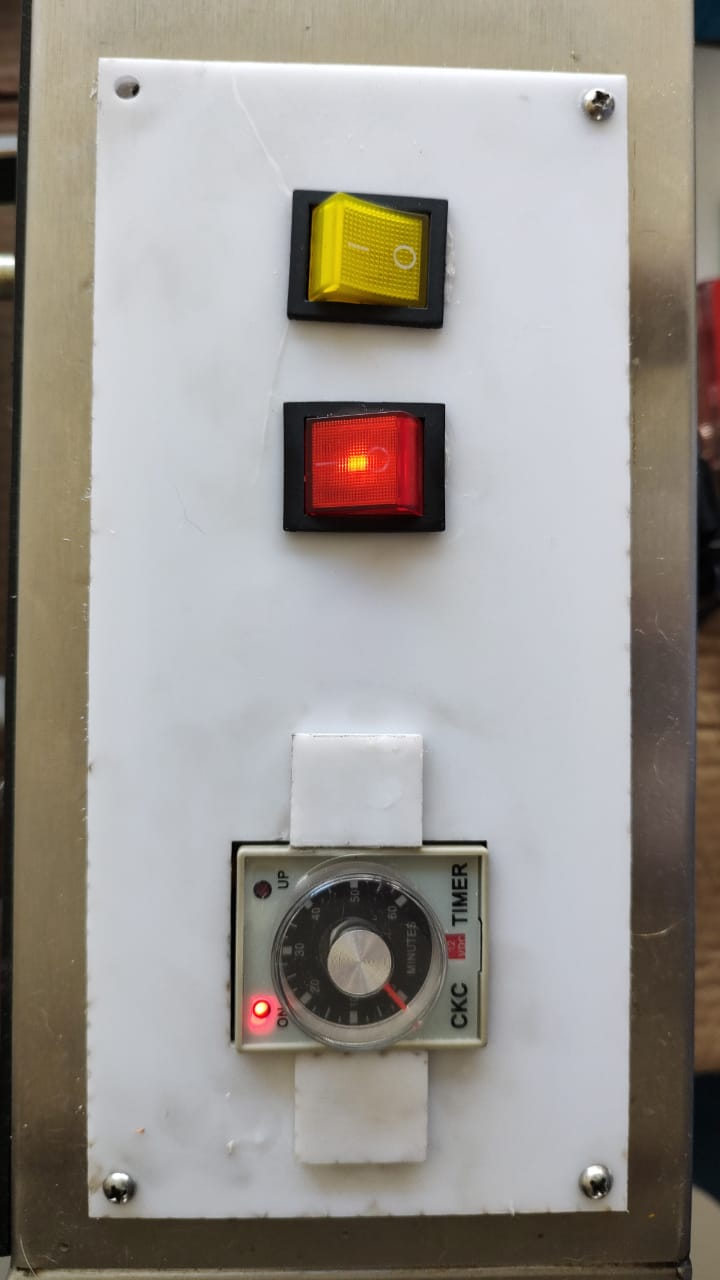
\includegraphics[angle=270, scale=0.21]{Figs/200.jpg}
	\caption{Indicador Luminoso}
	\label{fig:indicador}
\end{figure}

Se presiona el pulsador anteriormente mencionado, y se genera la conmutación del relé para la activación del motor, el cual se encuentra conectado a una caja reductora, que transmite la energía a tres engranajes rectos como se presentan en la Figura \ref{fig:caja}.

\begin{figure}[ht]
	\centering
	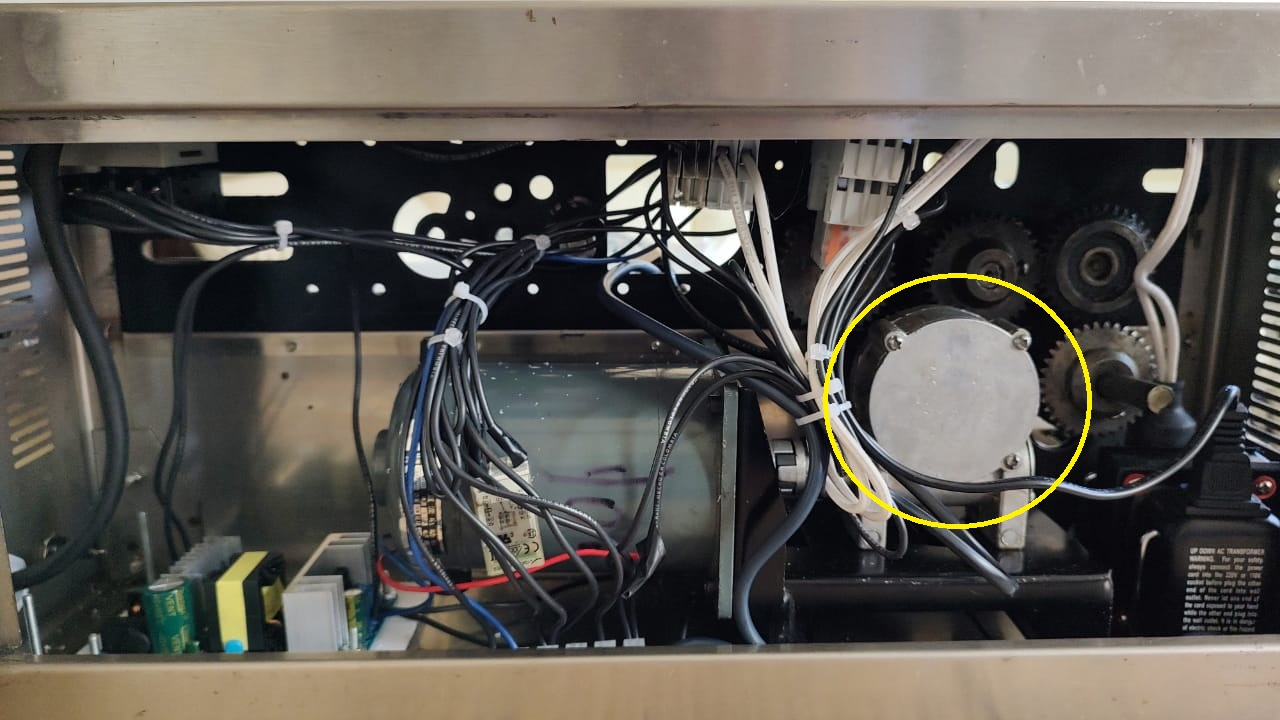
\includegraphics[scale=0.13]{Figs/201.jpg}
	\caption{Caja Reductora De Transmisión A Engranajes Rectos}
	\label{fig:caja}
\end{figure}

En donde el último engranaje se encuentra conectado, y transmite la energía a uno de los rodillos tensores de la banda transportadora, mediante un eje, como se aprecia en la Figura \ref{fig:eje}, con el fin de generar el movimiento de la banda. 

\newpage
\begin{figure}[ht]
	\centering
	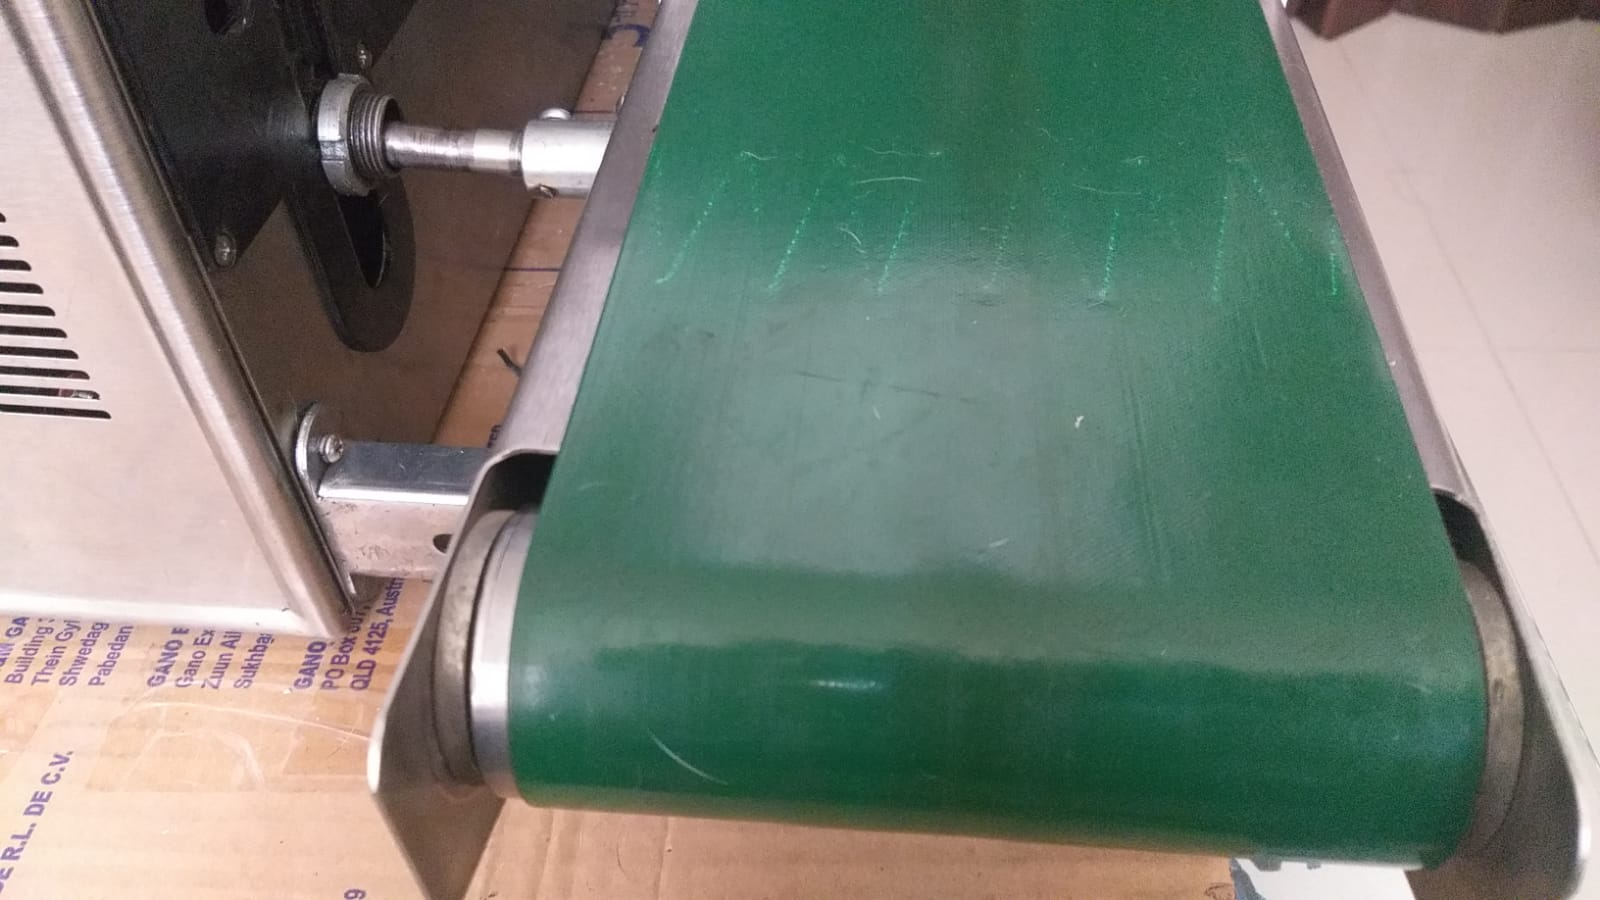
\includegraphics[angle=270, scale=0.21]{Figs/202.jpg}
	\caption{Conexión Engranajes y Rodillo Tensor}
	\label{fig:eje}
\end{figure}


Una vez se inicia el movimiento de la banda transportadora, este seguirá hasta que el tubérculo entre en contacto con el con la luz infrarroja del sensor foto eléctrico, como se observa en la Figura \ref{fig:sensor}, cuando el sensor detecte el tubérculo, la señal enviada detendrá la banda y activara un timer de un segundo, esto con el fin de permitir que la cámara tome la foto del tubérculo, y la envié a la red neuronal para su análisis el cual se explicará en la sección \textit{6.5.2 Implementación en Sistema Embedido}. Culminado el tiempo establecido en el timer, la banda continuara su movimiento para desplazar y continuar con la clasificación de los tubérculos.

\begin{figure}[ht]
	\centering
	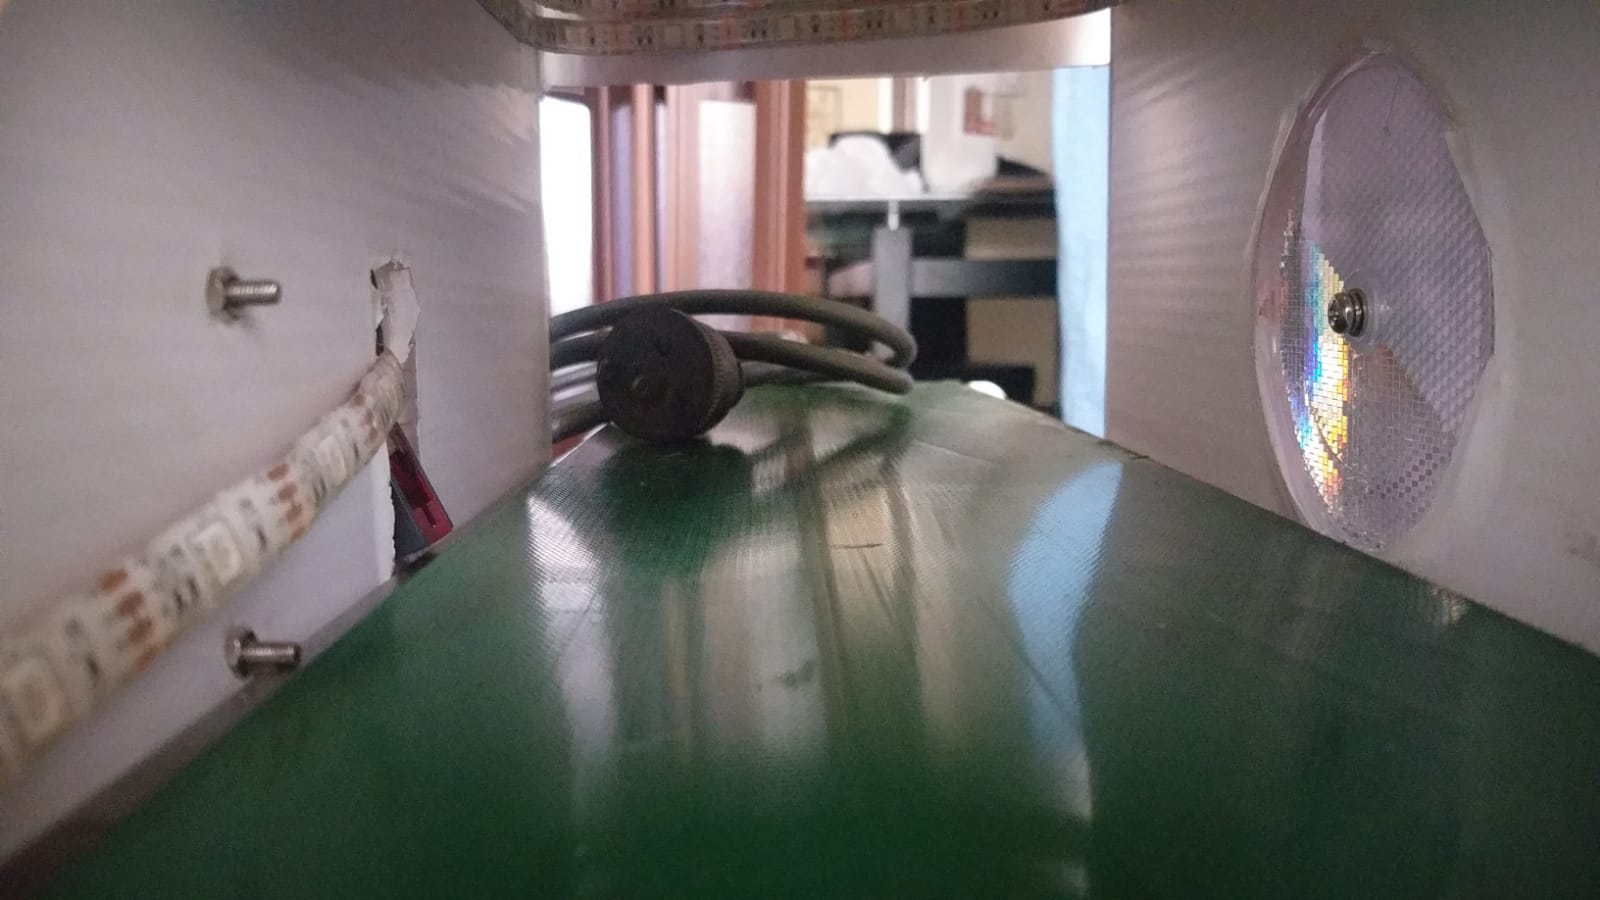
\includegraphics[scale=0.15]{Figs/203.jpg}
	\caption{Detección del sensor fotoeléctrico}
	\label{fig:sensor}
\end{figure}


\subsection{Implementación en Sistema Embebido}

Para el funcionamiento del algoritmo en tiempo real, en el prototipo construido, se utilizó una tarjeta de desarrollo Nvidia Jetson Nano $2 \ GB$, debido a que cuenta con una tarjeta gráfica y está diseñada para ejecutar modelos de redes neuronales. La implementación del algoritmo, debido a que la red fue entrenada con imágenes de tubérculos de papa estáticas, se realizó de igual forma.\\

El algoritmo captura una foto desde la webcam, realiza el procesamiento en la red neuronal y posteriormente, la clasificación por tamaño. Los resultados de cada imágen son mostrados por consola y la imágen capturada es guardada en formato $.jpg$, con la información de las predicciones, para verificar si la clasificación fue correcta. La imagen \ref{fig:implementacion}, muestra una de las papas pasando dentro de las estructura hecha para la clasificación.

\begin{figure}[ht]
	\centering
	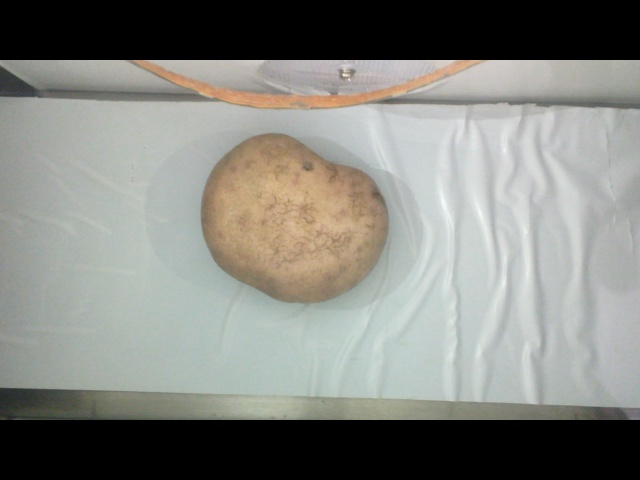
\includegraphics[scale=0.25]{Figs/implementacion.jpg}
	\caption{Tubérculo de Papa Dentro de La Estructura}
	\label{fig:implementacion}
\end{figure}

Se realizó un experimento con 50 papas de las diferentes clases, para verificar la precisión del algoritmo. La Tabla \ref{table:res} muestra los resultados de algunas de las papas utilizadas.

\begin{table}[ht]
	\centering
	\begin{tabular}{|cc|cc|}
		\hline
		\multicolumn{2}{|c|}{Real}                 & \multicolumn{2}{c|}{Prediccion}           \\ \hline
		\multicolumn{1}{|c|}{Clase}   & Tamaño     & \multicolumn{1}{c|}{Clase}   & Tamaño     \\ \hline
		\multicolumn{1}{|c|}{Clase 1} & Grande     & \multicolumn{1}{c|}{Clase 1} & Mediano    \\ \hline
		\multicolumn{1}{|c|}{Clase 1} & Muy Grande & \multicolumn{1}{c|}{Clase4}  & Muy Grande \\ \hline
		\multicolumn{1}{|c|}{Clase 4} & Mediana    & \multicolumn{1}{c|}{Clase 4} & Mediana    \\ \hline
		\multicolumn{1}{|c|}{Clase 3} & Grande     & \multicolumn{1}{c|}{Clase 3} & Grande     \\ \hline
		\multicolumn{1}{|c|}{Clase 2} & Mediana    & \multicolumn{1}{c|}{Clase 2} & Mediana    \\ \hline
		\multicolumn{1}{|c|}{Clase 1} & Mediana    & \multicolumn{1}{c|}{Clase 2} & Grande     \\ \hline
		\multicolumn{1}{|c|}{Clase 4} & Grande     & \multicolumn{1}{c|}{Clase 3} & Grande     \\ \hline
		\multicolumn{1}{|c|}{Clase 3} & Mediana    & \multicolumn{1}{c|}{Clase 3} & Mediana    \\ \hline
		\multicolumn{1}{|c|}{Clase 1} & Mediana    & \multicolumn{1}{c|}{Clase 1} & Mediana    \\ \hline
	\end{tabular}
	\caption{Resultados Papas Predichas}
	\label{table:res}
\end{table}


De las 50 papas utilizadas para la verificación, se obtuvo un resultado de $80\%$ de clases con correcta predicción y $88\%$ de tamaños correctamente clasificados. Esto da una precisión total de $85\%$ para las papas que fueron correctamente clasificadas en ambas categorías.\\

El tiempo de ejecución del algoritmo, desde el momento en el que toma la foto y la procesa, hasta que realiza la clasificación, varia entre los $2$ y $3$ segundos. El tiempo que demora la papa en llegar desde el comienzo de la banda transportadora, hasta la posición dentro de la estructura de análisis, es de $7$ segundos, por lo tanto, se puede asumir un tiempo promedio de $10$ segundos en analizar 1 tubérculo de papa. Este prototipo clasificaría $100$ tubérculos de papa cada $15$ minutos.	 	

\chapter{Conclusiones y Trabajo Futuro}

Debido a que el desarrollo del proyecto es un prototipo, la máquina puede ser mejorada para realizar la clasificación mecánica de las diferentes categorías, de igual forma, se puede implementar un variador para que la banda sea más rápida que el movimiento actual, mejorando así la velocidad de clasificación.\\

La red neuronal artificial que se obtuvo con una precisión superior al $83\%$, puede ser mejorada de tal manera que se puedan obtener precisiones superiores al $90\%$, para mejorar los resultados de las predicciones finales. Esto se puede lograr enriqueciendo el \textit{Dataset}, mejorando la distribución de los datos iniciales, de manera que sean proporcionales entre sí y realizando una optimización de hiperparámetros, teniendo en cuenta diferentes parámetros utilizados en este proyecto. Si se desea realizar una mejor optimización, el poder de computo necesario para realizarla debe ser muy superior, en las condiciones actuales, la optimización tomó un tiempo de $6$ horas por cada modelo en el que se aplicó.\\

Los tiempos de ejecución del algoritmo implementado en el sistema embebido, se deben mejorar, para que el prototipo sea viable en la agricultura de precisión. Además, se debe mejorar la capacidad de procesamiento en la tarjeta de desarrollo escogida y mejorar la sintaxis y consumo de memoria por parte del diseño del algoritmo hecho en \textit{Python}.










